\chapter{函数的限定展开}

这一章我们首先介绍函数的局部比较, 然后介绍函数的限定展开. 最后介绍函数限定展开在不定型极限的计算、函数局部极值与函数图形研究中的重要应用.

\section{函数的局部比较}

在许多数学问题中, 我们经常要对两个函数进行局部比较、 研究函数的局部性态, 为此我们介绍函数的三个局部比较关系概念,即: 大 $O$ 关系、小 $o$ 关系与等价关系.

以下我们设 $X \subset  \mathbf{R}$ 是任一非空 集合, $a \in  \overline{\mathbf{R}}$ 是 $X$ 的一个聚点.

\section*{1. 大 $O$ 关系}

定义 设 $f,g : X \rightarrow  \mathbf{R}$ 是任意两个函数,我们称函数 $f$ 当 $x \rightarrow$  $a$ 时关于函数 $g$ 是大 $O$ 关系,记为 $f = O\left( g\right) \left( {x \rightarrow  a}\right)$ ,如果存在一个函数 $h : X \rightarrow  \mathbf{R}$ 及 $a$ 的一个邻域 $U$ ,使得

1) $f\left( x\right)  = g\left( x\right) h\left( x\right) ,\forall x \in  X \cap  U$ ;

2) $\left| {h\left( x\right) }\right|  \leq  M,\;\forall x \in  X \cap  U$ . (这里 $M > 0$ )

容易验证下述简单结论:

若 $g\left( x\right)  \neq  0,\forall x \in  X \cap  U$ ,则
\begin{align*}
	&f = O\left( g\right) \left( {x \rightarrow  a}\right)\\
	&\Leftrightarrow  \exists M > 0,\forall x \in  X \cap  U,\left| \frac{f\left( x\right) }{g\left( x\right) }\right|  \leq  M.
\end{align*}

换句话说,当 $g$ 在 $a$ 的邻域内不等于 0 时,则 $f = O\left( g\right) \left( {x \rightarrow  a}\right)$ 当且

仅当函数 $\frac{f}{g}$ 在 $a$ 处是局部有界的.

特别地, $f = O\left( 1\right) \left( {x \rightarrow  a}\right)$ 表明 $f$ 在 $a$ 处是局部有界。

例 1 1 ) $x\sin \frac{1}{x} = O\left( x\right) \;\left( {x \rightarrow  0}\right)$ .
\begin{align*}
	&\text{ 2) arctg }\frac{1}{x} = O\left( 1\right) \left( {x \rightarrow  0}\right) \text{ . }\\
	&\text{ 3) }x + {x}^{2}\cos x = O\left( {x}^{2}\right) \;\left( {x \rightarrow   \pm  \infty }\right) \text{ . }\\
	&\text{ 4) }\frac{\operatorname{arctg}x}{1 + {x}^{2}} = O\left( \frac{1}{{x}^{2}}\right) \;\left( {x \rightarrow   \pm  \infty }\right) \text{ . }
\end{align*}

定理 $8 \cdot  1 \cdot  1$ 设 $f,g,\varphi ,\psi  : X \rightarrow  \mathbf{R}$ 是任意四个函数,并且
$$f = O\left( \varphi \right) \left( {x \rightarrow  a}\right) ,g = O\left( \psi \right) \left( {x \rightarrow  a}\right) ,$$

则

1) ${fg} = O\left( {\varphi \psi }\right) \left( {x \rightarrow  a}\right)$ ,

2) 若 $\psi  = O\left( \varphi \right) \left( {x \rightarrow  a}\right)$ ,则 $f + g = O\left( \varphi \right) \left( {x \rightarrow  a}\right)$ .

证明 因为 $f = O\left( \varphi \right) ,g = O\left( \psi \right) \left( {x \rightarrow  a}\right)$ ,所以存在可个函数 $h,k : X \rightarrow  \mathbf{R}$ 及 $a$ 的一个邻域 $U$ 与正数 $M$ ,使得 $\forall x \in  X \cap  U$ ,
\begin{align*}
	&f\left( x\right)  = \varphi \left( x\right) h\left( x\right) ,g\left( x\right)  = \psi \left( x\right) k\left( x\right) ,\\
	&\left| {h\left( x\right) }\right|  \leq  M,\left| {k\left( x\right) }\right|  \leq  M.
\end{align*}

于是
\begin{align*}
	&\text{ 1) }f\left( x\right) g\left( x\right)  = \varphi \left( x\right) \psi \left( x\right)  \cdot  h\left( x\right) k\left( x\right) ,\forall x \in  X \cap  U\text{ , }\\
	&\left| {h\left( x\right) k\left( x\right) }\right|  \leq  {M}^{2},\;\forall x \in  X \cap  U.
\end{align*}

因此 ${fg} = O\left( {\varphi \psi }\right)$ .

2) 若 $\psi  = O\left( \varphi \right) \left( {x \rightarrow  a}\right)$ ,则存在函数 $s : X \rightarrow  \mathbf{R}$ 及正数 $K$ 使得
$$\psi \left( x\right)  = \varphi \left( x\right) s\left( x\right) ,\;\left| {s\left( x\right) }\right|  \leq  K,\;\forall x \in  X \cap  U.$$

于是
\begin{align*}
	&f\left( x\right)  + g\left( x\right)  = \varphi \left( x\right) h\left( x\right)  + \psi \left( x\right) k\left( x\right)\\
	&= \varphi \left( x\right) \left\lbrack  {h\left( x\right)  + s\left( x\right) k\left( x\right) }\right\rbrack  ,\;\forall x \in  X \cap  U,\\
	&\left| {\dot{h}\left( x\right)  + s\left( x\right) k\left( x\right) }\right|  \leq  \left| {h\left( x\right) }\right|  + \left| {s\left( x\right) }\right| \left| {\dot{k}\left( x\right) }\right|\\
	&\leq  M\left( {1 + K}\right) ,\;\forall x \in  X \cap  U.
\end{align*}

因此 $f + g = O\left( \varphi \right) \;\left( {x \rightarrow  a}\right)$

推论 1) $O\left( {x}^{n}\right)  + O\left( {x}^{m}\right)  = O\left( {x}^{n}\right) \;\left( {x \rightarrow  0}\right) \;\left( {n \leq  m}\right)$ ,

2) $O\left( {x}^{n}\right)  + O\left( {x}^{m}\right)  = O\left( {x}^{m}\right) \;\left( {x \rightarrow   \pm  \infty }\right) \;\left( {n \leq  m}\right)$ .

证明 事实上,若 $n \leq  m$ ,则
$${x}^{m} = O\left( {x}^{n}\right) \left( {x \rightarrow  0}\right) ,{x}^{n} = O\left( {x}^{m}\right) \;\left( {x \rightarrow   \pm  \infty }\right) .$$

于是,若令 $f = O\left( {x}^{n}\right) ,g = O\left( {x}^{m}\right)$ ,则由上述定理
\begin{align*}
	&f + g = O\left( {x}^{n}\right)  + O\left( {x}^{m}\right)  = O\left( {x}^{n}\right) \;\left( {x \rightarrow  0}\right) ,\\
	&f + g = O\left( {x}^{n}\right)  + O\left( {x}^{m}\right)  = O\left( {x}^{m}\right) \;\left( {x \rightarrow   \pm  \infty }\right) .
\end{align*}

\section*{2. 小o关系}

定义 设 $f,g : X \rightarrow  \mathbf{R}$ 是任意两个函数,我们称函数 $f$ 当 $x \rightarrow$  $a$ 时关于函数 $g$ 是小 $o$ 关系,记为 $f = o\left( g\right) \left( {x \rightarrow  a}\right)$ ,如果存在一个函数 $h : X \rightarrow  \mathbf{R}$ 及 $a$ 的一个邻域 $U$ ,使得

1) $f\left( x\right)  = g\left( x\right) h\left( x\right) ,\forall x \in  X \cap  U$ ;

2) $\mathop{\lim }\limits_{{x \rightarrow  a}}h\left( x\right)  = 0$ .

显然,若 $g\left( x\right)  \neq  0,\forall x \in  X \cap  U$ ,则
$$f = o\left( g\right) \left( {x \rightarrow  a}\right)  \Leftrightarrow  \mathop{\lim }\limits_{{x \rightarrow  a}}\frac{f\left( x\right) }{g\left( x\right) } = 0.$$

特别地, 我们有
$$f = o\left( 1\right) \left( {x \rightarrow  a}\right)  \Leftrightarrow  \mathop{\lim }\limits_{{x \rightarrow  a}}f\left( x\right)  = 0$$

$\Leftrightarrow  f$ 是 $\langle a,0\rangle$ 型无穷小.

例 2 1) ${x}^{n}\sin \frac{1}{x} = o\left( x\right) \;\left( {x \rightarrow  0,n > 1}\right)$ .

2) $\operatorname{tg}x - \sin x = o\left( {\sin x}\right) \;\left( {x \rightarrow  0}\right)$ .

3) ${x}^{ \circ  } = o\left( {a}^{x}\right) \;\left( {x \rightarrow   + \infty ,a > 1}\right)$ .

4) ${a}^{-x} = o\left( {x}^{a}\right) \;\left( {x \rightarrow   + \infty ,a > 1}\right)$ .

5) $\log x = o\left( {x}^{a}\right) \;\left( {x \rightarrow   + \infty ,\alpha  > 0}\right)$ .

6) $\log x = o\left( {x}^{a}\right) \;\left( {x \rightarrow  {0}^{ + },\;\alpha  < 0}\right)$ .

定理 $8 \cdot  1 \cdot  2$ 设 $f,g,\varphi ,\psi  : X \rightarrow  \mathbf{R}$ 是任意四个函数.

1) 若 $f = O\left( \varphi \right) ,g = o\left( \psi \right)$ ,则 ${fg} = o\left( {\varphi \psi }\right) \;\left( {x \rightarrow  a}\right)$ .

2) 若 $f = o\left( \varphi \right) ,g = o\left( \varphi \right)$ ,则 $f + g = o\left( \varphi \right) \;\left( {x \rightarrow  a}\right)$ .

3) 若 $f = o\left( g\right) ,g = O\left( \varphi \right)$ ,则 $f = o\left( \varphi \right) \;\left( {x \rightarrow  a}\right)$ .

4) 若 $f = O\left( g\right) ,g = o\left( \varphi \right)$ ,则 $f = o\left( \varphi \right) \;\left( {x \rightarrow  a}\right)$ .

证明 1) 设 $f = O\left( \varphi \right) ,g = o\left( \psi \right) ,\left( {x \rightarrow  a}\right)$ 则存在函数 $h,k$ , $X \rightarrow  \mathbf{R}$ 及 $a$ 的一个邻域 $U$ 使得
\begin{align*}
	&f\left( x\right)  = \varphi \left( x\right) h\left( x\right) ,g\left( x\right)  = \psi \left( x\right) k\left( x\right) ,\;\forall x \in  X \cap  U,\\
	&\left| {h\left( x\right) }\right|  \leq  M,\;\forall x \in  X \cap  U,\mathop{\lim }\limits_{{x \rightarrow  a}}k\left( x\right)  = 0.
\end{align*}

于是
\begin{align*}
	&f\left( x\right) g\left( x\right)  = \left( {\varphi \left( x\right) \psi \left( x\right) }\right) \left( {h\left( x\right) k\left( x\right) }\right) ,\forall x \in  X \cap  U,\\
	&\mathop{\lim }\limits_{{x \rightarrow  a}}h\left( x\right) k\left( x\right)  = 0.
\end{align*}

因此 ${fg} = o\left( {\varphi \psi }\right) \left( {x \rightarrow  a}\right)$ .

类似地可证其他结论.

例 3 设 $n,m \in  \mathbf{N}$ . 并且 $f = o\left( {x}^{n}\right) ,g = o\left( {x}^{m}\right) \left( {x \rightarrow  0}\right)$ ,则

1) ${fg} = o\left( {x}^{n + m}\right) \;\left( {x \rightarrow  0}\right)$ .

2) $f = o\left( {x}^{m}\right) \;\left( {x \rightarrow  0,m < n}\right)$ .

3) $f + g = o\left( {x}^{m}\right) \;\left( {x \rightarrow  0,m < n}\right)$ .

事实上,1) 是上述定理 $8 \cdot  1 \cdot  {21}$ ) 的直接结论,

现设 $m < n$ . 于是 ${x}^{n} = o\left( {x}^{m}\right) \left( {x \rightarrow  0}\right)$ ,从而由 $f = o\left( {x}^{n}\right) (x \rightarrow$ 0 ) 及 ${x}^{n} = o\left( {x}^{m}\right) \left( {x \rightarrow  0}\right)$ 推得
$$f = o\left( {x}^{m}\right) \left( {x \rightarrow  0}\right) ,f + g = o\left( {x}^{m}\right) \left( {x \rightarrow  0}\right) .$$

\section*{3. 等价关系}

定义 设 $f,g : X \rightarrow  \mathbf{R}$ 是任意两个函数,我们称函数 $f$ 与函数 $g$ 当 $x \rightarrow  a$ 时是等价的,记为 $f \sim  g\left( {x \rightarrow  a}\right)$ ,如果存在一个函数 $h : X$  $\rightarrow  \mathbf{R}$ 及 $a$ 的一个邻域 $U$ ,使得

1) $f\left( x\right)  = g\left( x\right) h\left( x\right) ,\forall x \in  X \cap  U$ ;

2) $\mathop{\lim }\limits_{{x \rightarrow  a}}h\left( x\right)  = 1$ .

由此定义直接推出,若 $g\left( x\right)  \neq  0,\forall x \in  X \cap  U$ ,则
$$f \sim  g\left( {x \rightarrow  a}\right)  \Leftrightarrow  \mathop{\lim }\limits_{{x \rightarrow  a}}\frac{f\left( x\right) }{g\left( x\right) } = 1.$$

例 4 1) $\sin x \sim  x,\operatorname{sh}x \sim  x\;\left( {x \rightarrow  0}\right)$ .

2) $1 - \cos x \sim  \frac{1}{2}{x}^{2}$ , $\operatorname{ch}x - 1 \sim  \frac{1}{2}{x}^{2}\;\left( {x \rightarrow  0}\right)$ .

3) $\operatorname{tg}x \sim  x$ , th $x \sim  x\;\left( {x \rightarrow  0}\right)$ .
$$\text{ 4) }\log \left( {1 + x}\right)  \sim  {e}^{x} - 1\;\left( {x \rightarrow  0}\right) \text{ . }$$

定理 $8 \cdot  1 \cdot  3$ 若 $\mathcal{F}\left( X\right)$ 表示所有定义在 $X$ 上的实值函数的集合,我们在 $\mathcal{F}\left( X\right)$ 上定义关系 $\mathcal{B}$ 如下:
$$\forall f,g \in  \mathcal{F}\left( X\right) ,f\mathcal{B}g \Leftrightarrow  f \sim  g\left( {x \rightarrow  a}\right) .$$

则 $\mathcal{R}$ 是 $\mathcal{F}\left( X\right)$ 上的一个等价关系.

证明 1) 自反性. 显然 $\forall f \in  \mathcal{F}\left( X\right) ,f \sim  f\left( {x \rightarrow  a}\right)$ . 因此 $f\mathcal{R}f$ .

2) 对称性. 若 $f\mathcal{B}g$ ,则 $f \sim  g\left( {x \rightarrow  a}\right)$ ,于是由定义知,存在函数 $h : X \rightarrow  \mathbf{R}$ 及 $a$ 的一个邻域 $U$ 使得
$$f\left( x\right)  = g\left( x\right) h\left( x\right) ,\;\forall x \in  X \cap  U,\;\mathop{\lim }\limits_{{x \rightarrow  a}}h\left( x\right)  = 1.$$

于是我们可以假设 $h\left( x\right)  \neq  0,\forall x \in  X \cap  U$ ,从而
\begin{align*}
	&g\left( x\right)  = f\left( x\right) \frac{1}{h\left( x\right) },\;\forall x \in  X \cap  U,\\
	&\mathop{\lim }\limits_{{x \rightarrow  a}}\frac{1}{h\left( x\right) } = 1.
\end{align*}

因此 $g \sim  f\left( {x \rightarrow  a}\right)$ ,即 $g\mathcal{R}f$ .

3) 传递性. 若 $f\mathcal{B}g,g\mathcal{B}h$ ,则 $f \sim  g,g \sim  h\left( {x \rightarrow  a}\right)$ . 于是存在函数 $\varphi ,\psi  : X \rightarrow  \mathbf{R}$ 及 $a$ 的一个邻域 $U$ 使得
\begin{align*}
	&f\left( x\right)  = g\left( x\right) \varphi \left( x\right) ,g\left( x\right)  = h\left( x\right) \psi \left( x\right) ,\;\forall x \in  X \cap  U,\\
	&\mathop{\lim }\limits_{{x \rightarrow  a}}\varphi \left( x\right)  = 1,\;\mathop{\lim }\limits_{{x \rightarrow  a}}\psi \left( x\right)  = 1.
\end{align*}

因此
\begin{align*}
	&f\left( x\right)  = h\left( x\right) \varphi \left( x\right) \psi \left( x\right) ,\forall x \in  X \cap  U,\\
	&\mathop{\lim }\limits_{{x \rightarrow  a}}\varphi \left( x\right) \psi \left( x\right)  = 1
\end{align*}

从而 $f \sim  h\left( {x \rightarrow  a}\right)$ ,即 $f\mathcal{B}h$ .

因此 $\mathcal{B}$ 是 $\mathcal{F}\left( X\right)$ 上的一个等价关系.

定理 $8 \cdot  1 \cdot  4$ 设 ${f}_{1},{f}_{2},{g}_{1},{g}_{2} : X \rightarrow  \mathbf{R}$ 是任意四个函数.

1) 若 ${f}_{1} \sim  {g}_{1},{f}_{2} \sim  {g}_{2}\left( {x \rightarrow  a}\right)$ ,则 ${f}_{1}{f}_{2} \sim  {g}_{1}{g}_{2}\left( {x \rightarrow  a}\right)$ .

2) 若 ${f}_{1} \sim  {g}_{1},{f}_{2} \sim  {g}_{2}\left( {x \rightarrow  a}\right)$ ,并且存在 $a$ 的一个邻域 $V$ 使得 ${g}_{1}\left( x\right) {g}_{2}\left( x\right)  > 0,\;\forall x \in  X \cap  V$ ,则 ${f}_{1} + {f}_{2} \sim  {g}_{1} + {g}_{2}\left( {x \rightarrow  a}\right)$ .

证明 因为 ${f}_{1} \sim  {g}_{1},{f}_{2} \sim  {g}_{2}\left( {x \rightarrow  a}\right)$ ,所以存在两个函数 $h,k$ : $X \rightarrow  \mathbf{R}$ 及 $a$ 的一个邻域 $U$ 使得
\begin{align*}
	&{f}_{1}\left( x\right)  = {g}_{1}\left( x\right) h\left( x\right) ,\\
	&{f}_{2}\left( x\right)  = {g}_{2}\left( x\right) k\left( x\right) ,\;\forall x \in  X \cap  U,\\
	&\mathop{\lim }\limits_{{x \rightarrow  a}}h\left( x\right)  = 1,\;\mathop{\lim }\limits_{{x \rightarrow  a}}k\left( x\right)  = 1.
\end{align*}

于是
\begin{align*}
	&{f}_{1}\left( x\right) {f}_{2}\left( x\right)  = \left( {{g}_{1}\left( x\right) {g}_{2}\left( x\right) }\right) \left( {h\left( x\right) k\left( x\right) }\right) ,\\
	&\forall x \in  X \cap  U,\\
	&\mathop{\lim }\limits_{{x \rightarrow  a}}h\left( x\right) k\left( x\right)  = 1
\end{align*}

因此 ${f}_{1}{f}_{2} \sim  {g}_{1}{g}_{2}\left( {x \rightarrow  a}\right)$ .

此外,若令 $h\left( x\right)  = 1 + {\varepsilon }_{1}\left( x\right) ,k\left( x\right)  = 1 + {\varepsilon }_{2}\left( x\right) ,\forall x \in  X$ ,则 $\mathop{\lim }\limits_{{x \rightarrow  a}}{\varepsilon }_{1}\left( x\right)  = \mathop{\lim }\limits_{{x \rightarrow  a}}{\varepsilon }_{2}\left( x\right)  = 0$ ,并且
\begin{align*}
	&{f}_{1}\left( x\right)  = {g}_{1}\left( x\right)  + {g}_{1}\left( x\right) {\varepsilon }_{1}\left( x\right) ,\\
	&{f}_{2}\left( x\right)  = {g}_{2}\left( x\right)  + {g}_{2}\left( x\right) {\varepsilon }_{2}\left( x\right) ,\;\forall x \in  X \cap  U\\
	&{f}_{1}\left( x\right)  + {f}_{2}\left( x\right)  = \left\lbrack  {{g}_{1}\left( x\right)  + {g}_{2}\left( x\right) }\right\rbrack\\
	&+ \left\lbrack  {{g}_{1}\left( x\right) {\varepsilon }_{1}\left( x\right)  + {g}_{2}\left( x\right) {\varepsilon }_{2}\left( x\right) }\right\rbrack  ,\\
	&\forall x \in  X \cap  U.
\end{align*}

由假设 ${g}_{1}\left( x\right) {g}_{2}\left( x\right)  > 0,\forall x \in  X \cap  V$ ,所以
\begin{align*}
	&{f}_{1}\left( x\right)  + {f}_{2}\left( x\right)  = \left\lbrack  {{g}_{1}\left( x\right)  + {g}_{2}\left( x\right) }\right\rbrack  \left\lbrack  {1 + \frac{{g}_{1}\left( x\right) }{{g}_{1}\left( x\right)  + {g}_{2}\left( x\right) }{\varepsilon }_{1}\left( x\right) }\right.\\
	&\left. {+\frac{{g}_{2}\left( x\right) }{{g}_{1}\left( x\right)  + {g}_{2}\left( x\right) }{\varepsilon }_{2}\left( x\right) }\right\rbrack  \text{ , }\\
	&\forall x \in  X \cap  U \cap  V.
\end{align*}

并且由于 $\forall x \in  X \cap  U \cap  V,{g}_{1}\left( x\right)$ 与 ${g}_{2}\left( x\right)$ 同号,故
\begin{align*}
	&\left| {\frac{{g}_{1}\left( x\right) }{{g}_{1}\left( x\right)  + {g}_{2}\left( x\right) }{\varepsilon }_{1}\left( x\right)  + \frac{{g}_{2}\left( x\right) }{{g}_{1}\left( x\right)  + {g}_{2}\left( x\right) }{\varepsilon }_{2}\left( x\right) }\right|\\
	&\leq  \left| \frac{{g}_{1}\left( x\right) }{{g}_{1}\left( x\right)  + {g}_{2}\left( x\right) }\right| \left| {{\varepsilon }_{1}\left( x\right) }\right|\\
	&+ \left| \frac{{g}_{2}\left( x\right) }{{g}_{1}\left( x\right)  + {g}_{2}\left( x\right) }\right| \left| {{\varepsilon }_{2}\left( x\right) }\right|\\
	&\leq  \left| {{\varepsilon }_{1}\left( x\right) }\right|  + \left| {{\varepsilon }_{2}\left( x\right) }\right| .
\end{align*}

于是 $\mathop{\lim }\limits_{{x \rightarrow  a}}\left\lbrack  {\frac{{g}_{1}\left( x\right) }{{g}_{1}\left( x\right)  + {g}_{2}\left( x\right) }{\varepsilon }_{1}\left( x\right)  + \frac{{g}_{2}\left( x\right) }{{g}_{1}\left( x\right)  + {g}_{2}\left( x\right) }{\varepsilon }_{2}\left( x\right) }\right\rbrack   = 0$ ,从

iii
\begin{align*}
	&\mathop{\lim }\limits_{{x \rightarrow  a}}\left\lbrack  {1 + \frac{{g}_{1}\left( x\right) }{{g}_{1}\left( x\right)  + {g}_{2}\left( x\right) }{\varepsilon }_{1}\left( x\right) }\right.\\
	&\left. {+\frac{{g}_{2}\left( x\right) }{{g}_{1}\left( x\right)  + {g}_{2}\left( x\right) }{\varepsilon }_{2}\left( x\right) }\right\rbrack   = 1.
\end{align*}

因此 ${f}_{1} + {f}_{2} \sim  {g}_{1} + {g}_{2}\left( {x \rightarrow  a}\right)$ .

附注: 若将上述定理中结论 2 ) 的条件: “ ${g}_{1}\left( x\right) {g}_{2}\left( x\right)  > 0$ ” 换成 ${g}_{1}\left( x\right) {g}_{2}\left( x\right)  < 0,\forall x \in  X \cap  V$ ,则一般说来结论
$${x}_{1} + {f}_{2} \sim  {g}_{1} + {g}_{2}{\left( x \rightarrow  a\right) }^{n}$$

不再成立.

例 5 由于 $1 - {x}^{3} = \left( {1 - x}\right) \left( {1 + x + {x}^{2}}\right)$ ,故
$$1 - {x}^{3} \sim  1 - x\left( {x \rightarrow  0}\right) \text{ 且 }x - 1 \sim  x - 1\left( {x \rightarrow  0}\right)$$

但是
$$\left( {1 - {x}^{3}}\right)  + \left( {x - 1}\right)  = x - {x}^{3},\left( {1 - x}\right)  + \left( {x - 1}\right)  = 0,$$

显然 $x - {x}^{3}$ 与 0 当 $x \rightarrow  0$ 时不等价,其原因是 $1 - x$ 与 $x - 1$ 不同号.

定理 8.1.5 设 $f,g : X \rightarrow  \mathbf{R}$ 是任意两个函数,若 $f \sim  g(x \rightarrow$  $\left. \mathbf{a}\right)$ ,并且 $\mathop{\lim }\limits_{{x \rightarrow  a}}g\left( x\right)  = A \in  \overline{\mathbf{R}}$ . 则
$$\mathop{\lim }\limits_{{x \rightarrow  a}}f\left( x\right)  = A$$

证明 因为 $f \sim  g\left( {x \rightarrow  a}\right)$ ,所以存在函数 $h : X \rightarrow  \mathbf{R}$ 及 $a$ 的一个邻域 $U$ 使得
$$f\left( x\right)  = g\left( x\right) h\left( x\right) ,\;\forall x \in  X \cap  U,\mathop{\lim }\limits_{{x \rightarrow  a}}h\left( x\right)  = 1.$$

由于 $\mathop{\lim }\limits_{{x \rightarrow  a}}g\left( x\right)  = A \in  \overline{\mathbf{R}}$ ,故当 $A \in  \mathbf{R}$ 时
$$\mathop{\lim }\limits_{{x \rightarrow  a}}f\left( x\right)  = \mathop{\lim }\limits_{{x \rightarrow  a}}g\left( x\right)  \cdot  \mathop{\lim }\limits_{{x \rightarrow  a}}h\left( x\right)  = A \cdot  1 = A;$$

当 $A =  \pm  \infty$ 时,直接从定义可证 $\mathop{\lim }\limits_{{x \rightarrow  a}}f\left( x\right)  = A$ .

结合定理 $8 \cdot  1 \cdot  4$ 与定理 $8 \cdot  1 \cdot  5$ 可知,在计算函数极限 $\mathop{\lim }\limits_{{r \rightarrow  \infty }}f\left( x\right)$ 时,可以对 $f\left( x\right)$ 中的因子用等价的因子代换而不影响极限值.

例 6 计算 $\mathop{\lim }\limits_{{x \rightarrow  0}}\frac{1 - {\cos }^{n}x}{{x}^{2}}\left( {n \in  \mathbf{N}}\right)$ .

因为
\begin{align*}
	&\frac{1 - {\cos }^{n}x}{{x}^{2}} = \frac{\left( {1 - \cos x}\right) \left( {1 + \cos x + \cdots  + {\cos }^{n - 1}x}\right) }{{x}^{2}},\\
	&1 - \cos x - \frac{1}{2}{x}^{2}\;\left( {x \rightarrow  0}\right) ,
\end{align*}

所以
\begin{align*}
	&\mathop{\lim }\limits_{{x \rightarrow  0}}\frac{1 - \cos x}{{x}^{2}} = \mathop{\lim }\limits_{{x \rightarrow  0}}\frac{\frac{1}{2}{x}^{2}\left( {1 + \cos x + \cdots  + {\cos }^{n - 1}x}\right) }{{x}^{2}}\\
	&= \frac{n}{2}\text{ . }
\end{align*}

\section*{习 题}

1. 设 $f\left( x\right)  = \frac{{a}_{3}{x}^{3} + {a}_{2}{x}^{2} + {a}_{1}x + {a}_{0}}{{b}_{3}{x}^{3} + {b}_{2}{x}^{2} + {b}_{1}x + {b}_{0}}$ ,试选择常数 ${a}_{i},{b}_{i}(i = 0,1$ ,

2,3) 使得

1) $f = o\left( {x}^{2}\right) \left( {x \rightarrow  0}\right) ,2)f = O\left( {x}^{2}\right) \left( {x \rightarrow  0}\right)$ .

2. 在 $\mathcal{F}\left( X\right)$ 上定义关系 ${\mathcal{B}}_{1},{\mathcal{B}}_{2}$ 如下:

$\forall f,g \in  \mathcal{F}\left( X\right) ,f{\mathcal{R}}_{1}g \Leftrightarrow  f = O\left( g\right) \left( {x \rightarrow  a}\right) ,$

$\forall f,g \in  \mathcal{F}\left( X\right) ,f{\mathcal{B}}_{2}g \Leftrightarrow  f = o\left( g\right) \left( {x \rightarrow  a}\right) .$

试问 ${\mathcal{B}}_{1},{\mathcal{B}}_{2}$ 是 $\mathcal{F}\left( X\right)$ 上的等价关系吗?

3. 设 $f,g \in  \mathcal{F}\left( X\right)$ ,并且 $\mathop{\lim }\limits_{{x \rightarrow  a}}f\left( x\right)  = \mathop{\lim }\limits_{{x \rightarrow  a}}g\left( x\right)  = A$ .

1) 证明: 若 $A \in  \mathbf{R} - \{ 0\}$ ,则 $f \sim  g\left( {x \rightarrow  a}\right)$ .

2) 若 $A = 0$ 或 $A =  \pm  \infty$ ,则 $f \sim  g\left( {x \rightarrow  a}\right)$ 可以不成立. 试举例说明.

4. 设 $f,g \in  \mathcal{F}\left( X\right)$ 并且 $\operatorname{Ran}\left( f\right) ,\operatorname{Ran}\left( g\right)  \subset  {R}_{ * }^{ + }$ . 证明: 若 $f \sim  g(x \rightarrow$ a) 并且 $\mathop{\lim }\limits_{{x \rightarrow  a}}g\left( x\right)  = A \in  {R}_{ * }^{ \pm  }\{ 1\}$ ,则 $\log f \sim  \log g\left( {x \rightarrow  a}\right)$ .

5. 证明: $\forall f,g \in  \mathcal{F}\left( X\right)$ ,
$${e}^{f} \sim  {e}^{g} \Leftrightarrow  \mathop{\lim }\limits_{{x \rightarrow  a}}\left\lbrack  {f\left( x\right)  - g\left( x\right) }\right\rbrack   = 0.$$

6. 设 ${f}_{1},{f}_{2},{g}_{1},{g}_{2} \in  \mathcal{F}\left( X\right)$ ,并且 ${f}_{1} \sim  {g}_{1},{f}_{2} \sim  {g}_{2}\left( {x \rightarrow  a}\right)$ 证明:

1) 若 ${g}_{2} = o\left( {g}_{1}\right)$ ,则 ${f}_{1} + {f}_{2} \sim  {g}_{1}\left( {x \rightarrow  a}\right)$ .

2) 若存在 $\alpha  \neq   - 1$ 使得 ${g}_{2} \sim  \alpha {g}_{1}\left( {x \rightarrow  a}\right)$ ,则 ${f}_{1} + {f}_{2} \sim  \left( {1 + \alpha }\right) {g}_{1}(x \rightarrow$  $a)$ .

3) 若 ${g}_{2} \sim   - {g}_{1}\left( {x \rightarrow  a}\right)$ ,则 ${f}_{1} + {f}_{2} = o\left( {g}_{1}\right) \left( {x \rightarrow  a}\right)$ .

4) 利用上述结论证明:
\begin{align*}
	&\operatorname{ch}x \sim  \frac{{e}^{x}}{2},\operatorname{sh}x \sim  \frac{{e}^{x}}{2}\left( {x \rightarrow   + \infty }\right) ,\\
	&\operatorname{ch}x \sim  \frac{{e}^{-x}}{2},\operatorname{sh}x \sim   - \frac{{e}^{-x}}{2} \cdot  \left( {x \rightarrow   - \infty }\right) ,\\
	&\operatorname{Argch}x \sim  \log x\left( {x \rightarrow   + \infty }\right) ,\\
	&\operatorname{Argsh}x \sim  \log x\left( {x \rightarrow   + \infty }\right) .
\end{align*}

\section{函数的限定展开}

\section*{1. 问题的提出}

我们假设函数 $f : X \rightarrow  \mathbf{R}$ 在 ${x}_{0} \in  X$ 处可导. 根据定理 $6 \cdot  1 \cdot  2$ ,

1) $f\left( x\right)  = f\left( {x}_{0}\right)  + \varphi \left( x\right) \left( {x - {x}_{0}}\right) ,\forall x \in  X$ ,

2) $\varphi$ 在 ${x}_{0}$ 处连续且 $\varphi \left( {x}_{0}\right)  = {f}^{\prime }\left( {x}_{0}\right)$ .

若令 $\varphi \left( x\right)  = {f}^{\prime }\left( {x}_{0}\right)  + \varepsilon \left( x\right) ,\forall x \in  X$ ,则 $\mathop{\lim }\limits_{{x \rightarrow  {x}_{0}}}\bar{\varepsilon }\left( x\right)  = 0$ ,因此
\begin{align*}
	&f\left( x\right)  = f\left( {x}_{0}\right)  + \left\lbrack  {{f}^{\prime }\left( {x}_{0}\right)  + \varepsilon \left( x\right) }\right\rbrack  \left( {x - {x}_{0}}\right)\\
	&= f\left( {x}_{0}\right)  + {f}^{\prime }\left( {x}_{0}\right) \left( {x - {x}_{0}}\right)  + \varepsilon \left( x\right) \left( {x - {x}_{0}}\right) ,\\
	&\forall x \in  X,
\end{align*}

或
$$f\left( x\right)  = f\left( {x}_{0}\right)  + {f}^{\prime }\left( {x}_{0}\right) \left( {x - {x}_{0}}\right)  + o\left( {x - {x}_{0}}\right) \;\left( {x \rightarrow  {x}_{0}}\right) .$$

这里 ${P}_{1}\left( {x - {x}_{0}}\right)  = f\left( {x}_{0}\right)  + {f}^{\prime }\left( {x}_{0}\right) \left( {x - {x}_{0}}\right)$ 是关于 $\left( {x - {x}_{0}}\right)$ 的一次多项式. 上述表达式表明一次多项式 ${P}_{1}$ 是函数 $f$ 在 $X \cap  U(U$ 是 ${x}_{0}$ 的一个邻域) 内的近似函数,其误差函数 $f - {P}_{1}$ 当 $x \rightarrow  {x}_{0}$ 时关于 $x - {x}_{0}$ 是小 $o$ 关系.

由此我们很自然想到,当 $f$ 在 ${x}_{0}$ 处有更高阶的导数时, $f$ 在 $X \cap  U$ 内可能会有关于 $x - {x}_{0}$ 更高次的多项式 ${P}_{n}\left( {x - {x}_{0}}\right)$ 作为它的近似函数,并且其误差函数 $f - {P}_{n}$ 当 $x \rightarrow  {x}_{0}$ 时关于 ${\left( x - {x}_{0}\right) }^{n}$ 是小 $o$ 关系.

上述分析启发我们引入函数局部限定展开的一般概念.

\section*{2. 函数限定展开的定义}

定义 设 $X \subset  \mathbf{R}$ 是任一非空集合, ${x}_{0} \in  X$ 是 $X$ 的一个聚点, $f : X \rightarrow  \mathbf{R}$ 是任一函数。若存在常数 ${a}_{0},{a}_{1},{a}_{2},\cdots ,{a}_{n}(n = 0,1$ , $2,\cdots )$ 使得
\begin{align*}
	&f\left( x\right)  = {a}_{0} + {a}_{1}\left( {x - {x}_{0}}\right)  + {a}_{2}{\left( x - {x}_{0}\right) }^{2} + \cdots\\
	&+ {a}_{n}{\left( x - {x}_{0}\right) }^{n} + o\left( {\left( x - {x}_{0}\right) }^{n}\right) \left( {x \rightarrow  {x}_{0}}\right) ,
\end{align*}

则我们称函数 $f$ 在 ${x}_{0}$ 的邻域内有一个 $n$ 阶的限于多项式的展开式 (以后简称为 $n$ 阶限定展开式).

显然,有两个问题我们必须研究:

1) 是否任意一个函数 $f : X \rightarrow  \mathbf{R}$ 在 ${x}_{0} \in  X$ 的邻域内有一个 $n$ 阶的限定展开式?

2) 如果有, 这种限定展开式是否唯一?

下面我们首先研究第二个问题, 即

\section*{3. 限定展开式的唯一性}

定理 $8 \cdot  2 \cdot  1$ 若函数 $f : X \rightarrow  \mathbf{R}$ 在 ${x}_{0} \in  X$ 的邻域内有一个 $n$ 阶限定展开式, 则这个展开式是唯一的.

证明 假设存在两组常数 ${a}_{0},{a}_{1},{a}_{2},\cdots ,{a}_{n}$ 与 ${b}_{0},{b}_{1},{b}_{2}$ , $\cdots ,{b}_{n}$ 使得
\begin{align*}
	&f\left( x\right)  = {a}_{0} + {a}_{1}\left( {x - {x}_{0}}\right)  + {a}_{2}{\left( x - {x}_{0}\right) }^{2} + \cdots\\
	&+ {a}_{n}{\left( x - {x}_{0}\right) }^{n} + o\left( {\left( x - {x}_{0}\right) }^{n}\right) \;\left( {x \rightarrow  {x}_{0}}\right) ,\\
	&f\left( x\right)  = {b}_{0} + {b}_{1}\left( {x - {x}_{0}}\right)  + {b}_{2}{\left( x - {x}_{0}\right) }^{2} + \cdots\\
	&+ {b}_{n}{\left( x - {x}_{0}\right) }^{n} + o\left( {\left( x - {x}_{0}\right) }^{n}\right) \;\left( {x \rightarrow  {x}_{0}}\right) .
\end{align*}

那末我们有
\begin{align*}
	&0 = \left( {{a}_{0} - {b}_{0}}\right)  + \left( {{a}_{1} - {b}_{1}}\right) \left( {x - {x}_{0}}\right)  + \left( {{a}_{2} - {b}_{2}}\right) {\left( x - {x}_{0}\right) }^{2}\\
	&+ \cdots  + \left( {{a}_{n} - {b}_{n}}\right) {\left( x - {x}_{0}\right) }^{n} + o\left( {\left( x - {x}_{0}\right) }^{n}\right) \left( {x \rightarrow  {x}_{0}}\right) .
\end{align*}

两边令 $x \rightarrow  {x}_{0}$ 取极限得到 $0 = {a}_{0} - {b}_{0}$ ,即 ${a}_{0} = {b}_{0}$ .

将 ${a}_{0} = {b}_{0}$ 代入上式后两边再除以 $x - {x}_{0}\left( {x \neq  {x}_{0}}\right)$ 得到
\begin{align*}
	&0 = \left( {{a}_{1} - {b}_{1}}\right)  + \left( {{a}_{2} - {b}_{2}}\right) \left( {x - {x}_{0}}\right)  + \cdots\\
	&+ \left( {{a}_{n} - {b}_{n}}\right) {\left( x - {x}_{0}\right) }^{n - 1} + o\left( {\left( x - {x}_{0}\right) }^{n - 1}\right) \;\left( {x \rightarrow  {x}_{0}}\right) .
\end{align*}

再令 $x \rightarrow  {x}_{0}$ 取极限,又得到 ${a}_{1} - {b}_{1} = 0$ ,即 ${a}_{1} = {b}_{1}$ .

重复上述方法,我们可逐次得到 ${a}_{2} = {b}_{2},\cdots ,{a}_{n} = {b}_{n}$ . 因此唯一性得证.

\section*{4. 限定展开式的两个简单性质}

定理 $8 \cdot  2 \cdot  2$ 若函数 $f : X \rightarrow  \mathbf{R}$ 在 ${x}_{0} \in  X$ 的邻域内有 $n > 1$ 阶的限定展开式,则 $\forall m \in  \mathbf{N}$ 且 $m < n,f$ 在 ${x}_{0}$ 的邻域内有 $m$ 阶限定展开式.

证明 因为 $f$ 在 ${x}_{0}$ 的邻域内有 $n$ 阶限定展开式,所以
\begin{align*}
	&f\left( x\right)  = {a}_{0} + {a}_{1}\left( {x - {x}_{0}}\right)  + {a}_{2}{\left( x - {x}_{0}\right) }^{2} + \cdots\\
	&+ {a}_{n}{\left( x - {x}_{0}\right) }^{n} + o\left( {\left( x - {x}_{0}\right) }^{n}\right) \;\left( {x \rightarrow  {x}_{0}}\right) .
\end{align*}

于是 $\forall m \in  \mathbf{N}$ 且 $m < n$ ,
\begin{align*}
	&{a}_{m + 1}{\left( x - {x}_{0}\right) }^{m + 1} + \cdots  + {a}_{n}{\left( x - {x}_{0}\right) }^{n} + o\left( {\left( x - {x}_{0}\right) }^{n}\right)\\
	&= o\left( {\left( x - {x}_{0}\right) }^{m}\right)  + o\left( {\left( x - {x}_{0}\right) }^{n}\right)\\
	&= o\left( {\left( x - {x}_{0}\right) }^{m}\right) \;\left( {x \rightarrow  {x}_{0}}\right) ,
\end{align*}

从而
\begin{align*}
	&f\left( x\right)  = {a}_{0} + {a}_{1}\left( {x - {x}_{0}}\right)  + {a}_{2}{\left( x - {x}_{0}\right) }^{2} + \cdots\\
	&+ {a}_{m}{\left( x - {x}_{0}\right) }^{m} + o\left( {\left( x - {x}_{0}\right) }^{m}\right) \;\left( {x \rightarrow  {x}_{0}}\right) .
\end{align*}

因此 $f$ 在 ${x}_{0}$ 的邻域内有 $m$ 阶限定展开式.

下面一个定理反映了具有限定展开式的函数的两个内在性质.

定理 $8 \cdot  2 \cdot  3$ 若函数 $f : X \rightarrow  \mathbf{R}$ 在 ${x}_{0}$ 的邻域内有一个 $n$ 阶限定展开式:
\begin{align*}
	&f\left( x\right)  = {a}_{0} + {a}_{1}\left( {x - {x}_{0}}\right)  + {a}_{2}{\left( x - {x}_{0}\right) }^{2} + \cdots\\
	&+ {a}_{n}{\left( x - {x}_{0}\right) }^{n} + o\left( {\left( x - {x}_{0}\right) }^{n}\right) \;\left( {x \rightarrow  {x}_{0}}\right) ,
\end{align*}

则

1) $f$ 在 ${x}_{0}$ 处连续,并且 ${a}_{0} = f\left( {x}_{0}\right)$ .

2 当 $n \geq  1$ 时, $f$ 在 ${x}_{0}$ 处可导,并且 ${a}_{1} = {f}^{\prime }\left( {x}_{0}\right)$ .

证明 1) 首先在上述限 定展开式 中令 $x \rightarrow  {x}_{0}$ 取极限得到 $\mathop{\lim }\limits_{{x \rightarrow  {x}_{0}}}f\left( x\right)  = {a}_{0}$ ,然后将 $x = {x}_{0}$ 代入展开式中即得到 ${a}_{0} = f\left( {x}_{0}\right)$ ,因此 $f$ 在 ${x}_{0}$ 处连续.

2) 若 $n \geq  1$ ,则由 1 )所证, ${a}_{0} = f\left( {x}_{0}\right)$ ,从而对 $x \neq  {x}_{0}$ ,我

们有
\begin{align*}
	&\frac{f\left( x\right)  - f\left( {x}_{0}\right) }{x - {x}_{0}} = {a}_{1} + {a}_{2}\left( {x - {x}_{0}}\right)  + \cdots\\
	&+ {a}_{n}{\left( x - {x}_{0}\right) }^{n - 1} + o\left( {\left( x - {x}_{0}\right) }^{n - 1}\right)\\
	&\left( {x \rightarrow  {x}_{0}}\right) \text{ . }
\end{align*}

令 $x \rightarrow  {x}_{0}$ 取极限得到
$$\mathop{\lim }\limits_{{x \rightarrow  {x}_{0}}}\frac{f\left( x\right)  - f\left( {x}_{0}\right) }{x - {x}_{0}} = {a}_{1}.$$

因此 $f$ 在 ${x}_{0}$ 处可导,并且 ${f}^{\prime }\left( {x}_{0}\right)  = {a}_{1}$ .

下面我们来研究前面提出的限定展开式的存在性.

\section*{5. 限定展开式的存在性}

\section*{1) Taylor-Young公式}

定理 $8 \cdot  2 \cdot  4$ 设 $I \subset  \mathrm{R}$ 是任一非空区间. ${x}_{0} \in  I$ 若函数 $f : I \rightarrow$  $\mathbf{R}$ 在 ${x}_{0}$ 处 $n$ 次可导,则 $f$ 在 ${x}_{0}$ 的邻域内有下述形式的 $n$ 阶限定展开式:
\begin{align*}
	&f\left( x\right)  = f\left( {x}_{0}\right)  + \frac{{f}^{\prime }\left( {x}_{0}\right) }{1!}\left( {x - {x}_{0}}\right)  + \frac{{f}^{\prime \prime }\left( {x}_{0}\right) }{2!}{\left( x - {x}_{0}\right) }^{2}\\
	&+ \cdots  + \frac{{f}^{\left( n\right) }\left( {x}_{0}\right) }{n!}{\left( x - {x}_{0}\right) }^{n} + o\left( {\left( x - {x}_{0}\right) }^{n}\right) \left( {x \rightarrow  {x}_{0}}\right) .
\end{align*}

此展开式称为 $f$ 在 ${x}_{0}$ 的邻域内的 Taylor-Young 公式.

证明 我们对 $n$ 用数学归纳法进行证明.

当 $n = 1$ 时,我们在本节开头证明了
$$f\left( x\right)  = f\left( {x}_{0}\right)  + {f}^{\prime }\left( {x}_{0}\right) \left( {x - {x}_{0}}\right)  + o\left( {x - {x}_{0}}\right) \;\left( {x \rightarrow  {x}_{0}}\right) .$$

现假设定理当 $n = k$ 时成立. 我们来证明当 $n = k + 1$ 时定理也成立.

首先由 ${f}^{\left( k + 1\right) }\left( {x}_{0}\right)$ 存在表明 $f$ 在 ${x}_{0}$ 的邻域内导函数 ${f}^{\prime }$ 在 ${x}_{0}$ 处 $k$ 次可导, 故由归纳法假设
\begin{align*}
	&{f}^{\prime }\left( x\right)  = {f}^{\prime }\left( {x}_{0}\right)  + \frac{{f}^{\prime \prime }\left( {x}_{0}\right) }{1!}\left( {x - {x}_{0}}\right)  + \cdots  + \frac{{f}^{\left( k + 1\right) }\left( {x}_{0}\right) }{k!}{\left( x - {x}_{0}\right) }^{k}\\
	&+ o\left( {\left( x - {x}_{0}\right) }^{k}\right) \left( {x \rightarrow  {x}_{0}}\right) ,
\end{align*}

从而
\begin{align*}
	&\mathop{\lim }\limits_{{x \rightarrow  {x}_{0}}}\frac{1}{{\left( x - {x}_{0}\right) }^{k}}\left\{  {{f}^{\prime }\left( x\right)  - \left\lbrack  {{f}^{\prime }\left( {x}_{0}\right)  + \frac{{f}^{\prime \prime }\left( {x}_{0}\right) }{1!}\left( {x - {x}_{0}}\right) }\right. }\right.\\
	&\left. \left. {+\cdots  + \frac{{f}^{\left( k + 1\right) }\left( {x}_{0}\right) }{k!}{\left( x - {x}_{0}\right) }^{k}}\right\rbrack  \right\}   = 0.
\end{align*}

于是由 ${\mathrm{L}}^{\prime }\mathrm{H}$ ospital法则我们得到
\begin{align*}
	&\mathop{\lim }\limits_{{x \rightarrow  {x}_{0}}}\frac{1}{{\left( x - {x}_{0}\right) }^{k + 1}}\left\{  {f\left( x\right)  - \left\lbrack  {f\left( {x}_{0}\right)  + \frac{{f}^{\prime }\left( {x}_{0}\right) }{1!}\left( {x - {x}_{0}}\right) }\right. }\right.\\
	&\left. \left. {+\cdots  + \frac{{f}^{\left( k + 1\right) }\left( {x}_{0}\right) }{\left( {k + 1}\right) !}{\left( x - {x}_{0}\right) }^{k + 1}}\right\rbrack  \right\}\\
	&= \mathop{\lim }\limits_{{x \rightarrow  {x}_{0}}}\frac{1}{\left( {k + 1}\right) {\left( x - {x}_{0}\right) }^{k}}\left\{  {{f}^{\prime }\left( x\right)  - \left\lbrack  {{f}^{\prime }\left( {x}_{0}\right)  + \frac{{f}^{\prime \prime }\left( {x}_{0}\right) }{1!}\left( {x - {x}_{0}}\right) }\right. }\right.\\
	&\left. \left. {+\cdots  + \frac{{f}^{\left( k + 1\right) }\left( {x}_{0}\right) }{k!}{\left( x - {x}_{0}\right) }^{k}}\right\rbrack  \right\}\\
	&= 0\text{ . }
\end{align*}

现在我们定义函数 $R : I \rightarrow  \mathbf{R}$ 如下:
$$R\left( x\right)  = \left\{  \begin{matrix} \frac{1}{{\left( x - {x}_{0}\right) }^{k + 1}}\left\{  {f\left( x\right)  - \left\lbrack  {f\left( {x}_{0}\right)  + \frac{{f}^{\prime }\left( {x}_{0}\right) }{1!}\left( {x - {x}_{0}}\right) }\right. }\right. & \\  \left. \left. {+\cdots  + \frac{{f}^{\left( k + 1\right) }\left( {x}_{0}\right) }{\left( {k + 1}\right) !}{\left( x - {x}_{0}\right) }^{k + 1}}\right\rbrack  \right\}  , & x \neq  {x}_{0}, \\  0, & x = {x}_{0}. \end{matrix}\right.$$

则
\begin{align*}
	&f\left( x\right)  - \left\lbrack  {f\left( {x}_{0}\right)  + \frac{{f}^{\prime }\left( {x}_{0}\right) }{1!}\left( {x - {x}_{0}}\right)  + \cdots }\right.\\
	&\left. {+\frac{{f}^{\left( k + 1\right) }\left( {x}_{0}\right) }{\left( {k + 1}\right) !}{\left( x - {x}_{0}\right) }^{k + 1}}\right\rbrack   = {\left( x - {x}_{0}\right) }^{k + 1}R\left( x\right) ,\\
	&\forall x \in  I,\left( *\right)\\
	&\mathop{\lim }\limits_{{x \rightarrow  {x}_{0}}}R\left( x\right)  = 0
\end{align*}

从而
\begin{align*}
	&f\left( x\right)  - \left\lbrack  {f\left( {x}_{0}\right)  + \frac{{f}^{\prime }\left( {x}_{0}\right) }{1!}\left( {x - {x}_{0}}\right)  + \cdots }\right.\\
	&\left. {+\frac{{f}^{\left( k + 1\right) }\left( {x}_{0}\right) }{\left( {k + 1}\right) !}{\left( x - {x}_{0}\right) }^{k + 1}}\right\rbrack   = o\left( {\left( x - {x}_{0}\right) }^{k + 1}\right)\\
	&\left( {x \rightarrow  {x}_{0}}\right) \text{ , }
\end{align*}

或
\begin{align*}
	&f\left( x\right)  = f\left( {x}_{0}\right)  + \frac{{f}^{\prime }\left( {x}_{0}\right) }{1!}\left( {x - {x}_{0}}\right)  + \cdots  + \frac{{f}^{\left( k + 1\right) }\left( {x}_{0}\right) }{\left( {k + 1}\right) !}{\left( x - {x}_{0}\right) }^{k + 1}\\
	&+ o\left( {\left( x - {x}_{0}\right) }^{k + 1}\right) \left( {x \rightarrow  {x}_{0}}\right) .
\end{align*}

这就表明定理当 $n = k + 1$ 时成立. 因此由数学归纳法知定理对任意的 $n \in  \mathbf{N}$ 都成立.

附注 1) 若令 $x = {x}_{0} + h$ ,则 $x \rightarrow  {x}_{0}$ 当且仅当 $h \rightarrow  0$ ,因此上面的Taylor-Young公式又可表示成下述形式:
\begin{align*}
	&f\left( {{x}_{0} + h}\right)  = f\left( {x}_{0}\right)  + \frac{{f}^{\prime }\left( {x}_{0}\right) }{1!}h + \frac{{f}^{\prime \prime }\left( {x}_{0}\right) }{2!}{h}^{2} + \cdots  + \frac{{f}^{\left( n\right) }\left( {x}_{0}\right) }{n!}{h}^{n}\\
	&+ o\left( {h}^{n}\right) \left( {h \rightarrow  0}\right) \text{ . }
\end{align*}

2) 若在上述 $\left( *\right)$ 式中令 $k + 1 = n$ ,则我们得到
\begin{align*}
	&f\left( x\right)  = f\left( {x}_{0}\right)  + \frac{{f}^{\prime }\left( {x}_{0}\right) }{1!}\left( {x - {x}_{0}}\right)  + \cdots  + \frac{{f}^{\left( n\right) }\left( {x}_{0}\right) }{n!}{\left( x - {x}_{0}\right) }^{n}\\
	&+ {\left( x - {x}_{0}\right) }^{n}R\left( x\right) ,\;\forall x \in  I,
\end{align*}

这里 $\mathop{\lim }\limits_{{x \rightarrow  {x}_{0}}}R\left( x\right)  = 0$ .

多项式 ${P}_{n}\left( {x - {x}_{0}}\right)  = \mathop{\sum }\limits_{{k = 0}}^{n}\frac{{f}^{\left( k\right) }\left( {x}_{0}\right) }{k!}{\left( x - {x}_{0}\right) }^{k}$ 称为函数 $f$ 在 ${x}_{0}$ 处的 $n$ 阶 Taylor-Young 多项式,而 ${\left( x - {x}_{0}\right) }^{n}R\left( x\right)$ 称为函数 $f$ 在 ${x}_{0}$ 处的 $n$ 阶Taylor-Young公式的余项.

显然这种余项 ${\left( x - {x}_{0}\right) }^{n}R\left( x\right)$ 对我们研究误差 $f\left( x\right)  - {P}_{n}(r$  $\left. {-{x}_{0}}\right)$ 毫无用处. 因为由 $R\left( x\right)$ 的定义可以看出它并没有为我们提供任何具体的信息. 因此下面我们来寻求 Taylor-Young 公式的更实用的余项.

2 )Cauchy积分型与Lagrange型余项

定理 $8 \cdot  2 \cdot  5$ 若函数 $f : I \rightarrow  \mathbf{R}$ 在区间 $I$ 上是 ${C}^{n}$ 类的 $\left( {n \geq  1}\right)$ , ${x}_{0} \in  I$ ,则下述展开式成立:

1) $f\left( x\right)  = f\left( {x}_{0}\right)  + \frac{{f}^{\prime }\left( {x}_{0}\right) }{1!}\left( {x - {x}_{0}}\right)  + \cdots$
\begin{align*}
	&+ \frac{{f}^{\left( n - 1\right) }\left( {x}_{0}\right) }{\left( {n - 1}\right) !}{\left( x - {x}_{0}\right) }^{n - 1}\\
	&+ {\int }_{{x}_{0}}^{x}\frac{{f}^{\left( n\right) }\left( t\right) }{\left( {n - 1}\right) !}{\left( x - t\right) }^{n - 1}{dt},\;\forall x \in  I,
\end{align*}

或
\begin{align*}
	&\text{ 2) }f\left( x\right)  = f\left( {x}_{0}\right)  + \frac{{f}^{\prime }\left( {x}_{0}\right) }{1!}\left( {x - {x}_{0}}\right)  + \cdots\\
	&+ \frac{{f}^{\left( n - 1\right) }\left( {x}_{0}\right) }{\left( {n - 1}\right) !}{\left( x - {x}_{0}\right) }^{n - 1} + \frac{{f}^{\left( n\right) }\left( c\right) }{n!}{\left( x - {x}_{0}\right) }^{n},\\
	&\forall x \in  I\text{ . }
\end{align*}

这里 $c$ 介于 ${x}_{0}$ 与 $x$ 之间.

(第一个展开式称为带Cauchy积分型余项
$${\int }_{{x}_{0}}^{x}\frac{{f}^{\left( n\right) }\left( t\right) }{\left( {n - 1}\right) !} \cdot  {\left( x - t\right) }^{n - 1}{dt}$$

的Taylor公式,第二个展开式称为带Lagrange型

余项 $\frac{{f}^{\left( n\right) }\left( c\right) }{n!}{\left( x - {x}_{0}\right) }^{n}$ 的 Taylor 公式).

证明 首先证明第一个展开式. 仍然对 $n$ 用数学归纳法证明.

当 $n = 1$ 时,展开式 1 )为
$$f\left( x\right)  = f\left( {x}_{0}\right)  + {\int }_{{x}_{0}}^{x}{f}^{\prime }\left( t\right) {dt},\;\forall x \in  I,$$

这正是我们已经证明了的Newton-Leibniz公式.

现假设当 $n = k$ 时,展开式 1 )成立. 我们来证明当 $n = k + 1$ 时, 展开式 1 )仍然成立.

由于 $f$ 在 $I$ 上是 ${C}^{k + 1}$ 类的,故利用分部积分法得到
\begin{align*}
	&{\int }_{{r}_{0}}^{x}\frac{{f}^{\left( k\right) }\left( t\right) }{\left( {k - 1}\right) !}{\left( x - t\right) }^{k - 1}{dt}\\
	&= {\left\lbrack  -\frac{{f}^{\left( k\right) }\left( t\right) }{k!}{\left( x - t\right) }^{k}\right\rbrack  }_{{x}_{0}}^{x} + {\int }_{{x}_{0}}^{t}\frac{{f}^{\left( k + 1\right) }\left( t\right) }{k!}{\left( x - t\right) }^{k}{dt}\\
	&= \frac{{f}^{\left( k\right) }\left( {x}_{0}\right) }{k!}{\left( x - {x}_{0}\right) }^{k} + {\int }_{{x}_{0}}^{\tau }\frac{{f}^{\left( k + 1\right) }\left( t\right) }{k!}{\left( x - t\right) }^{k}{dt},\\
	&\forall x \in  I.
\end{align*}

根据归纳法假设我们有
\begin{align*}
	&f\left( x\right)  = f\left( {x}_{0}\right)  + \frac{{f}^{\prime }\left( {x}_{0}\right) }{1!}\left( {x - {x}_{0}}\right)  + \frac{{f}^{\prime \prime }\left( {x}_{0}\right) }{2!}{\left( x - {x}_{0}\right) }^{2} + \cdots\\
	&+ \frac{{f}^{\left( k - 1\right) }\left( {x}_{0}\right) }{\left( {k - 1}\right) !}{\left( x - {x}_{0}\right) }^{k - 1} + {\int }_{{x}_{0}}^{x}\frac{{f}^{\left( k\right) }\left( t\right) }{\left( {k - 1}\right) !}{\left( x - t\right) }^{k - 1}{dt}\\
	&= f\left( {x}_{0}\right)  + \frac{{f}^{\prime }\left( {x}_{0}\right) }{1!}\left( {x - {x}_{0}}\right)  + \frac{{f}^{\prime \prime }\left( {x}_{0}\right) }{2!}{\left( x - {x}_{0}\right) }^{2} + \cdots\\
	&+ \frac{{f}^{\left( k - 1\right) }\left( {x}_{0}\right) }{\left( {k - 1}\right) !}{\left( x - {x}_{0}\right) }^{k - 1} + \frac{{f}^{\left( k\right) }\left( {x}_{0}\right) }{k!}{\left( x - {x}_{0}\right) }^{k}\\
	&+ {\int }_{{x}_{0}}^{x}\frac{{f}^{\left( k + 1\right) }\left( t\right) }{k!}{\left( x - t\right) }^{k}{dt},\;\forall x \in  I.
\end{align*}

此即表明当 $n = k + 1$ 时,展开式 1 )成立. 从而由数学归纳法知, $\forall n \in  N$ ,展开式 1 )成立.

为了证明展开式 2 ), 我们来计算余项
$${\int }_{{x}_{0}}^{x}\frac{{f}^{\left( n\right) }\left( t\right) }{\left( {n - 1}\right) !}{\left( x - t\right) }^{n - 1}{dt}$$

若 $x \geq  {x}_{0}$ ,则 ${\left( x - t\right) }^{n - 1} \geq  0$ ,根据第一积分中值公式,存在介于 ${x}_{0}$ 与 $x$ 之间的一点 $c$ 使得
\begin{align*}
	&{\int }_{{x}_{0}}^{x}\frac{{f}^{\left( n\right) }\left( t\right) }{\left( {n - 1}\right) !}{\left( x - t\right) }^{n - 1}{dt} = {f}^{\left( n\right) }\left( c\right) {\int }_{{x}_{0}}^{x}\frac{{\left( x - t\right) }^{n - 1}}{\left( {n - 1}\right) !}{dt}\\
	&= \frac{{f}^{\left( n\right) }\left( c\right) }{n!}{\left( x - {x}_{0}\right) }^{n}.
\end{align*}

将它代入展开式 1 )中得到
\begin{align*}
	&f\left( x\right)  = f\left( {x}_{0}\right)  + \frac{{f}^{\prime }\left( {x}_{0}\right) }{1!}\left( {x - {x}_{0}}\right)  + \cdots  + \frac{{f}^{\left( n - 1\right) }\left( {x}_{0}\right) }{\left( {n - 1}\right) !}{\left( x - {x}_{0}\right) }^{n - 1}\\
	&+ \frac{{f}^{\left( n\right) }\left( c\right) }{n!}{\left( x - {x}_{0}\right) }^{n},\\
	&\forall x \in  I\text{ 且 }x \geq  {x}_{0}.
\end{align*}

若 $x \leq  {x}_{0}$ ,则证明完全类似,因此 $\forall x \in  I$ ,展开 2) 成立.

附注 若 $0 \in  I$ ,则在上述两个展开式 1 )与 2 )中用 ${x}_{0} = 0$ 代入,我们得到下列两个展开式:
\begin{align*}
	&f\left( x\right)  = f\left( 0\right)  + \frac{{f}^{\prime }\left( 0\right) }{1!}x + \frac{{f}^{\prime \prime }\left( 0\right) }{2!}{x}^{2} + \cdots  + \frac{{f}^{\left( n - 1\right) }\left( 0\right) }{\left( {n - 1}\right) !}{x}^{n - 1}\\
	&+ {\int }_{0}^{x}\frac{{f}^{\left( n\right) }\left( t\right) }{\left( {n - 1}\right) !}{\left( x - t\right) }^{n - 1}{dt},\\
	&f\left( x\right)  = f\left( 0\right)  + \frac{{f}^{\prime }\left( 0\right) }{1!}x + \frac{{f}^{\prime \prime }\left( 0\right) }{2!}{x}^{2} + \cdots  + \frac{{f}^{\left( n - 1\right) }\left( 0\right) }{\left( {n - 1}\right) !}{x}^{n - 1}\\
	&+ \frac{{f}^{\left( n\right) }\left( c\right) }{n!}{x}^{n}.\;\left( {\forall x \in  I}\right)
\end{align*}

这里 $c$ 介于 0 与 $x$ 之间.

这两个展开式又称为 $f$ 的 Maclaurin 公式.

下面我们来研究余项的估计.

3)余项的估计

定理 $8 \cdot  2 \cdot  6$ 若函数 $f : I \rightarrow  \mathbf{R}$ 在区间 $I$ 上是 ${C}^{n}$ 类的, ${x}_{0} \in  I$ ,

并且存在常数 $M > 0$ 使得
$$\left| {{f}^{\left( n\right) }\left( x\right) }\right|  \leq  M,\;\forall x \in  I,$$

则我们有
\begin{align*}
	&f\left( x\right)  - \left\lbrack  {f\left( {x}_{0}\right)  + \frac{{f}^{\prime }\left( {x}_{0}\right) }{1!}\left( {x - {x}_{0}}\right)  + \cdots }\right.\\
	&\left. {+\frac{{f}^{\left( n - 1\right) }\left( {x}_{0}\right) }{\left( {n - 1}\right) !}{\left( x - {x}_{0}\right) }^{n - 1}}\right\rbrack   \leq  M\frac{{\left| x - {x}_{0}\right| }^{n}}{n!},\;\forall x \in  I.
\end{align*}

证明 由于 $f$ 在 $I$ 上是 ${C}^{n}$ 类的,故由定理 $8 \cdot  2 \cdot  5$ 有
\begin{align*}
	&f\left( x\right)  = f\left( {x}_{0}\right)  + \frac{{f}^{\prime }\left( {x}_{0}\right) }{1!}\left( {x - {x}_{0}}\right)  + \cdots  + \frac{{f}^{\left( n - 1\right) }\left( {x}_{0}\right) }{\left( {n - 1}\right) !}{\left( x - {x}_{0}\right) }^{n - 1}\\
	&+ \frac{{f}^{\left( n\right) }\left( c\right) }{n!}{\left( x - {x}_{0}\right) }^{n},\;\forall x \in  I.
\end{align*}

从而
\begin{align*}
	&f\left( x\right)  - \left\lbrack  {f\left( {x}_{0}\right)  + \frac{{f}^{\prime }\left( {x}_{0}\right) }{1!}\left( {x - {x}_{0}}\right)  + \cdots }\right.\\
	&\left. \left. {+\frac{{f}^{\left( n - 1\right) }\left( {x}_{0}\right) }{\left( {n - 1}\right) !}{\left( x - {x}_{0}\right) }^{n - 1}}\right\rbrack  \right\rbrack\\
	&= \left| {\frac{{f}^{\left( n\right) }\left( c\right) }{n!}{\left( x - {x}_{0}\right) }^{n}}\right|\\
	&\leq  \frac{M}{n!}{\left| x - {x}_{0}\right| }^{n},\forall x \in  I.
\end{align*}

\section*{习 题}

1. 设函数 $f : R \rightarrow  R$ 定义如下:
$$f\left( x\right)  = \left\{  \begin{array}{ll} 1 + x + \frac{{x}^{2}}{3} + {x}^{3}\sin \frac{1}{x}, & x \neq  0; \\  1, & x = 0. \end{array}\right.$$

证明: 函数 $f$ 在 $x = 0$ 的邻域内有一个 2 阶限定展开式 但 $f$ 在 $x = 0$ 处不是 2 次可导的.

2. 设函数 $f : {R}_{ * }^{ + } \rightarrow  R$ 定义如下:

$\forall x \in  {R}_{ * }^{ + },f\left( x\right)  = {x}^{p}\left\lbrack  \frac{1}{x}\right\rbrack$ ,这里 $p \in  N$ 且 $p > 3$ .

1) 证明: 函数 $f$ 可以连续延拓到 $x = 0$ ,并且延拓函数 $f$ 在 $x = 0$ 处可导.

2) 证明: 在 $x = 0$ 的任意邻域内都包含有函数 $f$ 的间断点. 由此推得 $f$ 在 $x = 0$ 的任意邻域内都有不可导点.

3) 证明: 函数 $f$ 在 $x = 0$ 的邻域内有 $p - 2$ 阶限定展开式.

3. 设函数 $f : I \rightarrow  R\left( {0 \in  I}\right)$ 在 $R$ 上是 ${C}^{\infty }$ 类的,并且 $\forall n \in  N,f\left( x\right)  =$  $o\left( {x}^{n}\right) \left( {x \rightarrow  0}\right)$ . 试问 $f$ 在 $x = 0$ 的邻域内是否恒等于 0 ? 举例说明.

4. 设 $I \in  \mathcal{N}\left( 0\right)$ , $f : I \rightarrow  R$ 满足下述条件:
$$\forall n \in  N,f\left( x\right)  = o\left( {x}^{n}\right) \;\left( {x \rightarrow  0}\right)$$

试问 $f$ 在 $I$ 上是 ${C}^{\infty }$ 类的吗? 考虑下述函数
$$f\left( x\right)  = \left\{  \begin{array}{ll} {e}^{-{x}^{2}}\sin \left( {e}^{\frac{1}{{x}^{2}}}\right) , & \text{ 若 }x \in  \rbrack 0, + \infty \lbrack , \\  0, & \text{ 若 }x \in  \rbrack  - \infty ,0\rbrack . \end{array}\right.$$

5. 设 $f,g : I \rightarrow  R$ 是任意两个函数,我们称函数 $f,g$ 在 $a \in  I$ 处是 $n$ 阶相等的, 如果
$$\mathop{\lim }\limits_{{x \rightarrow  a}}\frac{f\left( x\right)  - g\left( x\right) }{{\left( x - a\right) }^{n}} = 0\text{ 或 }f - g = o\left( {\left( x - a\right) }^{n}\right) \left( {x \rightarrow  a}\right) .$$

1) 证明: 若 $P,Q$ 是次数 $\leq  n$ 的关于(x - a)的多项式,并且 $P,Q$ 在 $a$ 处是 $n$ 阶相等的,则 $P = Q$ .

2) 若 $f$ 在 $a$ 处 $n$ 次可导,并且 $P$ 是次数 $\leq  n$ 的关于(x - a)的多项式,它在 $a$ 处与 $f$ 是 $n$ 阶相等,则
\begin{align*}
	&P\left( x\right)  = f\left( a\right)  + \frac{{f}^{\prime }\left( a\right) }{1!}\left( {x - a}\right)  + \frac{{f}^{\prime \prime }\left( a\right) }{2!}{\left( x - a\right) }^{2} + \cdots\\
	&+ \frac{{f}^{\left( n\right) }\left( a\right) }{n!}{\left( x - a\right) }^{n}.
\end{align*}

6. 设函数 $f : \left\lbrack  {a,b}\right\rbrack   \rightarrow  \mathrm{R}$ 在 $\left\lbrack  {a,b}\right\rbrack$ 上是 ${C}^{2}$ 类的,并且 ${f}^{\prime }\left( a\right)  = {f}^{\prime }\left( b\right)  =$ 0 . 证明: 存在 $\xi  \in  \rbrack a,b\lbrack$ 使得
$$\left| {{f}^{\prime \prime }\left( \xi \right) }\right|  \geq  \frac{4}{{\left( b - a\right) }^{2}}\left| {f\left( b\right)  - f\left( a\right) }\right| .$$

7. 设函数 $f : \left\lbrack  {0,2}\right\rbrack   \rightarrow  R$ 在 $\left\lbrack  {0,2}\right\rbrack$ 上是 ${C}^{2}$ 类的,并且 $\left| {f\left( x\right) }\right|  \leq  1$ , $\left| {{f}^{\prime \prime }\left( x\right) }\right|  \leq  1,\forall x \in  \left\lbrack  {0,2}\right\rbrack$ . 证明:
$$\left| {{f}^{\prime }\left( x\right) }\right|  \leq  2,\;\forall x \in  \left\lbrack  {0,2}\right\rbrack  .$$

8. 设函数 $f : \left\lbrack  {0,a}\right\rbrack   \rightarrow  \mathrm{R}$ 在 $\left\lbrack  {0,a}\right\rbrack$ 上 $n + 1$ 次可导,并且 ${f}^{\left( n + 1\right) }\left( x\right)$ 在 $x = 0$ 处右连续, ${f}^{\left( n + 1\right) }\left( 0\right)  \neq  0$ . $\forall x \in  \left\lbrack  {0,a}\right\rbrack$ ,令
$$f\left( x\right)  = f\left( 0\right)  + \frac{{f}^{\prime }\left( 0\right) }{1!}x + \cdots  + \frac{{f}^{\left( n - 1\right) }\left( 0\right) }{\left( {n - 1}\right) !}{x}^{n - 1} + \frac{{f}^{\left( n\right) }\left( \xi \right) }{n!}{x}^{n},$$

证明: $\mathop{\lim }\limits_{{x \rightarrow  {0}^{ + }}}\frac{\xi }{x} = \frac{1}{n + 1}$ .

9. 1) 利用Taylor公式证明: 对函数 $f : I \rightarrow  \mathbf{R},{x}_{0} \in  I$ ,若 ${f}^{\prime \prime }\left( {x}_{0}\right)$ 存在, 则 ${f}^{\prime \prime }\left( {x}_{0}\right)  = \mathop{\lim }\limits_{{h \rightarrow  0}}\frac{f\left( {{x}_{0} + h}\right)  + f\left( {{x}_{0} - h}\right)  - {2f}\left( {x}_{0}\right) }{{h}^{2}}$ .

2) 设
$$f\left( x\right)  = \left\{  \begin{array}{ll} {x}^{2}, & x \geq  0, \\   - {x}^{2}, & x \leq  0. \end{array}\right.$$

证明: $\mathop{\lim }\limits_{{h \rightarrow  0}}\frac{f\left( {0 + h}\right)  + f\left( {0 - h}\right)  - {2f}\left( 0\right) }{{h}^{2}}$ 存在,但 ${f}^{\prime \prime }\left( 0\right)$ 不存在.

10. 这个题目是要证明带 Schlömlich型余项的 Taylor 公式. 它是带 Lagrange型余项Taylor公式的推广.

设函数 $f : I \rightarrow  R$ 在区间 $I$ 上 $n$ 次连续可导,并且 $f$ 在 $I$ 的内部 $n + 1$ 次可导, $p \in  R$ 且 $P >  - 1.{x}_{0} \in  I$ ,证明: $\forall x \in  I$ ,
$$f\left( x\right)  = \mathop{\sum }\limits_{{k = 0}}^{n}\frac{{f}^{\left( k\right) }\left( {x}_{0}\right) }{k!}{\left( x - {x}_{0}\right) }^{k} + \frac{{f}^{\left( n + 1\right) }\left( c\right) }{\left( {p + 1}\right) n!}{\left( x - c\right) }^{n - p}{\left( x - a\right) }^{p + 1},$$

这里 $c$ 介于 ${x}_{0}$ 与 $x$ 之间. 为此我们建议

1) $\forall x \in  I$ 且 $x \neq  {x}_{0}$ ,令
\begin{align*}
	&F\left( t\right)  = f\left( x\right)  - f\left( t\right)  - \mathop{\sum }\limits_{{k = 1}}^{n}\frac{{f}^{\left( k\right) }\left( t\right) }{k!}{\left( x - t\right) }^{k} - \frac{{\left( x - t\right) }^{p + 1}}{{\left( x - {x}_{0}\right) }^{p + 1}}(f\left( x\right)\\
	&\left. {-\mathop{\sum }\limits_{{k = 0}}^{n}\frac{{f}^{\left( k\right) }\left( {x}_{0}\right) }{k!}{\left( x - {x}_{0}\right) }^{k}}\right)
\end{align*}

$\left( {t \in  I}\right)$ . 证明: 存在 $c$ ,它介于 ${x}_{0}$ 与 $x$ 之间使得 ${F}^{\prime }\left( c\right)  = 0$ .

2) 计算 ${F}^{\prime }\left( t\right)$ .

3) 由此推得我们的结论.

11. 设 $f \in  {C}^{2}\left( {R,R}\right)$ 且有上界, ${f}^{\prime \prime }\left( x\right)  \geq  0\left( {\forall x \in  R}\right)$ ,证明 $f$ 是常值函数.

12. 设 $f \in  {C}^{2}\left( {R,R}\right)$ 且 $f,{f}^{\prime \prime }$ 在 $R$ 上有界. 证明: ${f}^{\prime }$ 在 $R$ 上有界,并且满

足不等式
$${M}_{1}^{2} \leq  {M}_{0}{M}_{2}$$

这里 ${M}_{i} = \mathop{\sup }\limits_{{x \in  \mathbf{R}}}\left| {{f}^{\left( i\right) }\left( x\right) }\right| ,i = 0,1,2$ .

\section{函数限定展开的一般法则}

现在我们利用前面两节的理论来研究函数限定展开的实际方法.

\section*{1. 直接按定义展开}

这种方法一般只适用于比较简单的函数. 例如, 对某些基本初等函数,我们可以直接计算它们在 $x = 0$ 处的各阶导数以求出它们在 $x = 0$ 的邻域内的任意阶的限定展开式 (因为基本初等函数在各自定义域上都是 ${C}^{\infty }$ 类的).

例 1 正弦、余弦函数在 $x = 0$ 的邻域内的限定展开式.

因为 ${\sin }^{\left( 2n\right) }\left( 0\right)  = 0,{\sin }^{\left( 2n + 1\right) }\left( 0\right)  = {\left( -1\right) }^{n}$ ,
$${\cos }^{\left( 2n\right) }\left( 0\right)  = {\left( -1\right) }^{n},{\cos }^{\left( 2n + 1\right) }\left( 0\right)  = 0.\;\left( {n = 0,1,2,\cdots }\right)$$

所以它们在 $x = 0$ 的邻域内的限定展开式为
$$\sin x = x - \frac{{x}^{3}}{3!} + \frac{{x}^{5}}{5!} - \cdots  + {\left( -1\right) }^{n}\frac{{x}^{{2n} + 1}}{\left( {{2n} + 1}\right) !} + o\left( {x}^{{2n} + 2}\right)$$

$\left( {x \rightarrow  0}\right)$
$$\cos x = 1 - \frac{{x}^{2}}{2!} + \frac{{x}^{4}}{4!} - \cdots  + {\left( -1\right) }^{n}\frac{{x}^{2n}}{\left( {2n}\right) !} + o\left( {x}^{{2n} + 1}\right)$$

例 2 指数函数在 $x = 0$ 的邻域内的限定展开式.

因为 ${\left( {a}^{x}\right) }^{\left( n\right) } = {a}^{x}{\left( \log a\right) }^{n},{\left( {e}^{x}\right) }^{\left( n\right) } = {e}^{x},\forall n \in  \mathbf{N}$ ,所以 ${\left( {a}^{x}\right) }^{\left( n\right) }\left( 0\right)  = {\log }^{n}a,{\left( {e}^{x}\right) }^{\left( n\right) }\left( 0\right)  = 1\left( {0 < a \neq  1,\forall n \in  \mathbf{N}}\right)$ ,从而指数函数在 $x = 0$ 的邻域内的限定展开式为
$${a}^{x} = 1 + \frac{\log a}{1!}x + \frac{{\log }^{2}a}{2!}{x}^{2} + \cdots  + \frac{{\log }^{n}a}{n!}{x}^{n} + o\left( {x}^{n}\right)$$

$\left( {x \rightarrow  0}\right)$
$${e}^{x} = 1 + \frac{x}{1!} + \frac{{x}^{2}}{2!} + \cdots  + \frac{{x}^{n}}{n!} + o\left( {x}^{n}\right)$$

例3 函数 $x \mapsto  \log \left( {1 + x}\right) ,x >  - 1$ 在 $x = 0$ 的邻域内的限定展 开式.

直接计算我们得到
\begin{align*}
	&{\left\lbrack  \log \left( 1 + x\right) \right\rbrack  }^{\prime } = \frac{1}{1 + x},\\
	&{\left\lbrack  \log \left( 1 + x\right) \right\rbrack  }^{\prime \prime } = {\left( \frac{1}{1 + x}\right) }^{\prime } =  - \frac{1}{{\left( 1 + x\right) }^{2}},\\
	&{\left\lbrack  \log \left( 1 + x\right) \right\rbrack  }^{\prime \prime \prime } = {\left( -\frac{1}{{\left( 1 + x\right) }^{2}}\right) }^{\prime } = \frac{1 \cdot  2}{{\left( 1 + x\right) }^{3}},\\
	&{\left\lbrack  \log \left( 1 + x\right) \right\rbrack  }^{\left( 4\right) } = {\left( \frac{2}{{\left( 1 + x\right) }^{3}}\right) }^{\prime } =  - \frac{1 \cdot  2 \cdot  3}{{\left( 1 + x\right) }^{4}}.
\end{align*}

于是不难用数学归纳法证明
$${\left\lbrack  \log \left( 1 + x\right) \right\rbrack  }^{\left( n\right) } = {\left( -1\right) }^{n - 1}\frac{\left( {n - 1}\right) !}{{\left( 1 + x\right) }^{n}}.$$

从而
$${\left\lbrack  \log \left( 1 + x\right) \right\rbrack  }^{\left( n\right) }\left( 0\right)  = {\left( -1\right) }^{n - 1}\left( {n - 1}\right) !.$$

因此函数 $x \mapsto  \log \left( {1 + x}\right) ,x >  - 1$ 在 $x = 0$ 的邻域内的限定展开式为
\begin{align*}
	&\log \left( {1 + x}\right)  = x - \frac{{x}^{2}}{2} + \frac{{x}^{3}}{3} - \frac{{x}^{4}}{4} + \cdots  + {\left( -1\right) }^{n - 1}\frac{{x}^{n}}{n}\\
	&+ o\left( {x}^{n}\right) \left( {x \rightarrow  0}\right) \text{ . }
\end{align*}

例 4 幂函数 $x \mapsto  {\left( 1 + x\right) }^{a},x >  - 1$ 在 $x = 0$ 的邻域内的限定展开式.

若 $a = n \in  \mathbf{N}$ ,则
$${\left( 1 + x\right) }^{n} = 1 + {C}_{n}^{1}x + {C}_{n}^{2}{x}^{2} + \cdots  + {C}_{n}^{n}{x}^{n}.$$

若 $\alpha  \in  \mathbf{N}$ ,且 $\alpha  \neq  0$ . 则由于
\begin{align*}
	&{\left\lbrack  {\left( 1 + x\right) }^{\alpha }\right\rbrack  }^{\left( n\right) } = \alpha \left( {\alpha  - 1}\right) \left( {\alpha  - 2}\right) \cdots \left( {\alpha  - n + 1}\right) {\left( 1 + x\right) }^{\alpha  - n + 1},\\
	&\left( {\forall n \in  \mathbf{N}}\right)\\
	&{\left\lbrack  {\left( 1 + x\right) }^{\alpha }\right\rbrack  }^{\left( n\right) }\left( 0\right)  = \alpha \left( {\alpha  - 1}\right) \left( {\alpha  - 2}\right) \cdots \left( {\alpha  - n + 1}\right) ,
\end{align*}

故函数 $x \mapsto  {\left( 1 + x\right) }^{a},x >  - 1$ 在 $x = 0$ 的邻域内的限定展开式为:
\begin{align*}
	&{\left( 1 + x\right) }^{\alpha } = 1 + \frac{\alpha }{1!}x + \frac{\alpha \left( {\alpha  - 1}\right) }{2!}{x}^{2} + \cdots\\
	&+ \frac{a\left( {a - 1}\right) \cdots \left( {a - n + 1}\right) }{n!}{x}^{n} + o\left( {x}^{n}\right) \left( {x \rightarrow  0}\right) .
\end{align*}

特别地,当 $\alpha  =  - 1,\frac{1}{2}, - \frac{1}{2}$ 时,我们得到下列三个常用的限定展开式:
\begin{align*}
	&\frac{1}{1 + x} = 1 - x + {x}^{2} - {x}^{3} + \cdots  + {\left( -1\right) }^{n}{x}^{n} + o\left( {x}^{n}\right) \left( {x \rightarrow  0}\right) .\\
	&\sqrt{1 + x} = 1 + \frac{1}{2}x - \frac{1}{8}{x}^{2} + \cdots  + {\left( -1\right) }^{n - 1}\frac{1 \cdot  3 \cdot  \cdots  \cdot  \left( {{2n} - 3}\right) }{2 \cdot  4 \cdot  \cdots  \cdot  {2n}}{x}^{n}\\
	&+ o\left( {x}^{n}\right) \left( {x \rightarrow  0}\right) \text{ . }\\
	&\frac{1}{\sqrt{1 + x}} = 1 - \frac{1}{2}x + \frac{3}{8}{x}^{2} - \cdots  + {\left( -1\right) }^{n}\frac{1 \cdot  3 \cdot  \cdots  \cdot  \left( {{2n} - 1}\right) }{2 \cdot  4 \cdot  \cdots  \cdot  {2n}}{x}^{n}\\
	&+ o\left( {x}^{n}\right) \left( {x \rightarrow  0}\right) \text{ . }
\end{align*}

\section*{2. 和函数的限定展开}

定理 $8 \cdot  3 \cdot  1$ 设函数 $f,g : X \rightarrow  \mathbf{R}$ 在 $x = 0 \in  X$ 的邻域内有 $n$ 阶限定展开式:
\begin{align*}
	&f\left( x\right)  = {a}_{0} + {a}_{1}x + {a}_{2}{x}^{2} + \cdots  + {a}_{n}{x}^{n} + o\left( {x}^{n}\right) \left( {x \rightarrow  0}\right) ,\\
	&g\left( x\right)  = {b}_{0} + {b}_{1}x + {b}_{2}{x}^{2} + \cdots  + {b}_{n}{x}^{n} + o\left( {x}^{n}\right) \left( {x \rightarrow  0}\right) ,
\end{align*}

则函数 $f + g : X \rightarrow  \mathbf{R}$ 在 $x = 0$ 的邻域内也有 $n$ 阶限定展开式,并且
\begin{align*}
	&\left( {f + g}\right) \left( x\right)  = \left( {{a}_{0} + {b}_{0}}\right)  + \left( {{a}_{1} + {b}_{1}}\right) x + \left( {{a}_{2} + {b}_{2}}\right) {x}^{2} + \cdots\\
	&+ \left( {{a}_{n} + {b}_{n}}\right) {x}^{n} + o\left( {x}^{n}\right) \left( {x \rightarrow  0}\right) .
\end{align*}

\section*{证明 因为}
\begin{align*}
	&\left( {f + g}\right) \left( x\right)  = \left( {{a}_{0} + {b}_{0}}\right)  + \left( {{a}_{1} + {b}_{1}}\right) x + \left( {{a}_{2} + {b}_{2}}\right) {x}^{2} + \cdots\\
	&+ \left( {{a}_{n} + {b}_{n}}\right) {x}^{n} + o\left( {x}^{n}\right)  + o\left( {x}^{n}\right)\\
	&= \left( {{a}_{0} + {b}_{0}}\right)  + \left( {{a}_{1} + {b}_{1}}\right) x + \left( {{a}_{2} + {b}_{2}}\right) {x}^{2} + \cdots\\
	&+ \left( {{a}_{n} + {b}_{n}}\right) {x}^{n} + o\left( {x}^{n}\right) \;\left( {x \rightarrow  0}\right) .
\end{align*}

例5 考虑双曲正弦、余弦函数 $x \mapsto  \operatorname{sh}x,x \mapsto  \operatorname{ch}x,x \in$  $\mathbf{R}$ 在 $x = 0$ 的邻域内的限定展开式. 由于 $\operatorname{sh}x = \frac{1}{2}\left( {{e}^{x} - {e}^{-x}}\right)$ , $\operatorname{ch}x = \frac{1}{2}\left( {{e}^{x} + {e}^{-x}}\right)$ ,及
\begin{align*}
	&{e}^{x} = 1 + \frac{x}{1!} + \frac{{x}^{2}}{2!} + \frac{{x}^{3}}{3!} + \cdots  + \frac{{x}^{n}}{n!} + o\left( {x}^{n}\right) \left( {x \rightarrow  0}\right) ,\\
	&{e}^{-x} = 1 - \frac{x}{1!} + \frac{{x}^{2}}{2!} - \frac{{x}^{3}}{3!} + \cdots  + {\left( -1\right) }^{n}\frac{{x}^{n}}{n!} + o\left( {x}^{n}\right) \left( {x \rightarrow  0}\right) ,
\end{align*}

故由上述定理推得
\begin{align*}
	&2\operatorname{sh}x = \left( {1 - 1}\right)  + \left( {\frac{1}{1!} + \frac{1}{1!}}\right) x + \left( {\frac{1}{2!} - \frac{1}{2!}}\right) {x}^{2} + \left( {\frac{1}{3!} + \frac{1}{3!}}\right) {x}^{3} + \cdots\\
	&+ \left( {\frac{1}{n!} - {\left( -1\right) }^{n}\frac{1}{n!}}\right) {x}^{n} + o\left( {x}^{n}\right) \left( {x \rightarrow  0}\right) ,\\
	&2\operatorname{ch}x = \left( {1 + 1}\right)  + \left( {\frac{1}{1!} - \frac{1}{1!}}\right) x + \left( {\frac{1}{2!} + \frac{1}{2!}}\right) {x}^{2} + \left( {\frac{1}{3!} - \frac{1}{3!}}\right) {x}^{3} + \cdots\\
	&+ \left( {\frac{1}{n!} + {\left( -1\right) }^{n}\frac{1}{n!}}\right) {x}^{n} + o\left( {x}^{n}\right) \left( {x \rightarrow  0}\right) .
\end{align*}

因此
$$\operatorname{sh}x = x + \frac{1}{3!}{x}^{3} + \cdots  + \frac{1}{\left( {{2n} + 1}\right) !}{x}^{{2n} + 1} + o\left( {x}^{{2n} + 1}\right) .$$

$\left( {x \rightarrow  0}\right)$
$$\operatorname{ch}x = 1 + \frac{1}{2!}{x}^{2} + \frac{1}{4!}{x}^{4} + \cdots  + \frac{1}{\left( {2n}\right) !}{x}^{2n} + o\left( {x}^{2n}\right) .$$

\section*{3. 乘积函数的限定展开}

定理 $8 \cdot  3 \cdot  2$ 设函数 $f,g : X \rightarrow  \mathbf{R}$ 在 $x = 0 \in  X$ 的邻域内有 $n$ 阶

限定展开式:
\begin{align*}
	&f\left( x\right)  = {a}_{0} + {a}_{1}x + {a}_{2}{x}^{2} + \cdots  + {a}_{n}{x}^{n} + o\left( {x}^{n}\right) \left( {x \rightarrow  0}\right) ,\\
	&g\left( x\right)  = {b}_{0} + {b}_{1}x + {b}_{2}{x}^{2} + \cdots  + {b}_{n}{x}^{n} + o\left( {x}^{n}\right) \left( {x \rightarrow  0}\right) ,
\end{align*}

则函数 ${fg} : X \rightarrow  \mathbf{R}$ 在 $x = 0$ 的邻域内也有 $n$ 阶限定展开式,并且
\begin{align*}
	&{fg}\left( x\right)  = {a}_{0}{b}_{0} + \left( {{a}_{0}{b}_{1} + {a}_{1}{b}_{0}}\right) x + \left( {{a}_{0}{b}_{2} + {a}_{1}{b}_{1} + {a}_{2}{b}_{0}}\right) {x}^{2} + \cdots\\
	&+ \left( {{a}_{0}{b}_{n} + {a}_{1}{b}_{n - 1} + \cdots  + {a}_{n}{b}_{0}}\right) {x}^{n} + o\left( {x}^{n}\right) \left( {x \rightarrow  0}\right) .
\end{align*}

证明 直接将 $f$ 与 $g$ 的限定展开式相乘得到
\begin{align*}
	&{fg}\left( x\right)  = \left( {{a}_{0} + {a}_{1}x + {a}_{2}{x}^{2} + \cdots  + {a}_{n}{x}^{n}}\right) \left( {{b}_{0} + {b}_{1}x + {b}_{2}{x}^{2} + \cdots }\right.\\
	&\left. {+{b}_{n}{x}^{n}}\right)  + \left( {{a}_{0} + {a}_{1}x + {a}_{2}{x}^{2} + \cdots  + {a}_{n}{x}^{n} + o\left( {x}^{n}\right) }\right) o\left( {x}^{n}\right.\\
	&+ \left( {{b}_{0} + {b}_{1}x + {b}_{2}{x}^{2} + \cdots  + {b}_{n}{x}^{n} + o\left( {x}^{n}\right) }\right) o\left( {x}^{n}\right)\\
	&= {a}_{0}{b}_{0} + \left( {{a}_{0}{b}_{1} + {a}_{1}{b}_{0}}\right) x + \left( {{a}_{0}{b}_{2} + {a}_{1}{b}_{1} + {a}_{2}{b}_{0}}\right) {x}^{2} + \cdots\\
	&+ \left( {{a}_{0}{b}_{n} + {a}_{1}{b}_{n - 1} + \cdots  + {a}_{n}{b}_{0}}\right) {x}^{n}\\
	&+ \left\lbrack  {\left( {{a}_{1}{b}_{n} + {a}_{2}{b}_{n - 1} + \cdots  + {a}_{n}{b}_{1}}\right) {x}^{n + 1} + \cdots  + {a}_{n}{b}_{n}{x}^{2n}}\right.\\
	&+ \left( {{a}_{0} + {a}_{1}x + {a}_{2}{x}^{2} + \cdots  + {a}_{n}{x}^{n} + o\left( {x}^{n}\right) }\right) o\left( {x}^{n}\right)\\
	&\left. {+\left( {{b}_{0} + {b}_{1}x + {b}_{2}{x}^{2} + \cdots  + {b}_{n}{x}^{n} + o\left( {x}^{n}\right) }\right) o\left( {x}^{n}\right) }\right\rbrack
\end{align*}
$$\left( {x \rightarrow  0}\right) \text{ . }$$

而根据定理 $8 \cdot  1 \cdot  2$ 知,上式右边方括号 $\left\lbrack  {\cdots \cdots }\right\rbrack   = o\left( {x}^{n}\right) \left( {x \rightarrow  0}\right)$ , 因此
\begin{align*}
	&{fg}\left( x\right)  = {a}_{0}{b}_{0} + \left( {{a}_{0}{b}_{1} + {a}_{1}{b}_{0}}\right) x + \left( {{a}_{0}{b}_{2} + {a}_{1}{b}_{1} + {a}_{2}{b}_{0}}\right) {x}^{2} + \cdots\\
	&+ \left( {{a}_{0}{b}_{n} + {a}_{1}{b}_{n - 1} + \cdots  + {a}_{n}{b}_{0}}\right) {x}^{n} + o\left( {x}^{n}\right) \left( {x \rightarrow  0}\right) .
\end{align*}

例 6 求函数 $x \mapsto  \sin x\log \left( {1 + x}\right) \left( {x >  - 1}\right)$ 在 $x = 0$ 的邻域内的 5 阶限定展开式.

由 $\sin x$ 及 $\log \left( {1 + x}\right)$ 在 $x = 0$ 的邻域内的限定展开式可知,我们只需取
$$\sin x = x - \frac{{x}^{3}}{3!} + o\left( {x}^{4}\right) ,\log \left( {1 + x}\right)  = x - \frac{{x}^{2}}{2} + \frac{{x}^{3}}{3} - \frac{{x}^{4}}{4} + o\left( {x}^{4}\right) ,$$

于是
\begin{align*}
	&\sin x\log \left( {1 + x}\right)  = \left( {x - \frac{{x}^{3}}{3!} + o\left( {x}^{4}\right) }\right) \left( {x - \frac{{x}^{2}}{2} + \frac{{x}^{3}}{3} - \frac{{x}^{4}}{4} + o\left( {x}^{4}\right) }\right)\\
	&= {x}^{2} - \frac{1}{2}{x}^{3} + \left( {\frac{1}{3} - \frac{1}{3!}}\right) {x}^{4} + \left( {\frac{1}{2 \cdot  3!} - \frac{1}{4}}\right) {x}^{3}\\
	&+ O\left( {x}^{5}\right)\\
	&= {x}^{2} - \frac{1}{2}{x}^{3} + \frac{1}{6}{x}^{4} - \frac{1}{6}{x}^{5} + o\left( {x}^{5}\right) \left( {x \rightarrow  0}\right) .
\end{align*}

\section*{4. 商函数的限定展开}

定理 $8 \cdot  3 \cdot  3$ 设函数 $f,g : X \rightarrow  \mathbf{R}$ 在 $x = 0 \in  X$ 的邻域内有 $n$ 阶限定展开式,并且 $g\left( 0\right)  \neq  0$ ,则函数 $\frac{f}{g} : x \rightarrow  \mathbf{R}$ 在 $x = 0$ 的邻域内也有 $n$ 阶限定展开式.

证明 设
\begin{align*}
	&f\left( x\right)  = {a}_{0} + {a}_{1}x + {a}_{2}{x}^{2} + \cdots  + {a}_{n}{x}^{n} + o\left( {x}^{n}\right)\\
	&\left( {x \rightarrow  0}\right) \text{ . }\\
	&g\left( x\right)  = {b}_{0} + {b}_{1}x + {b}_{2}{x}^{2} + \cdots  + {b}_{n}{x}^{n} + o\left( {x}^{n}\right)
\end{align*}

由于 $g\left( 0\right)  \neq  0$ ,故 ${b}_{0} \neq  0$ . 于是在 $x = 0$ 的充分小邻域内 $g \neq  0$ . 令
\begin{align*}
	&P\left( x\right)  = {a}_{0} + {a}_{1}x + {a}_{2}{x}^{2} + \cdots  + {a}_{n}{x}^{n},\\
	&Q\left( x\right)  = {b}_{0} + {b}_{1}x + {b}_{2}{x}^{2} + \cdots  + {b}_{n}{x}^{n},
\end{align*}

由多项式的升幂除法知,存在两个多项式 $S\left( x\right) ,R\left( x\right)$ 使得
$$P\left( x\right)  = S\left( x\right) Q\left( x\right)  + {x}^{n + 1}R\left( x\right) ,$$

这里 $S\left( x\right)$ 的次数 $\leq  n$ . 于是
$$f\left( x\right)  - o\left( {x}^{n}\right)  = S\left( x\right) \left\lbrack  {g\left( x\right)  - o\left( {x}^{n}\right) }\right\rbrack   + {x}^{n + 1}R\left( x\right) \;\left( {x \rightarrow  0}\right) ,$$

或
$$f\left( x\right)  = S\left( x\right) g\left( x\right)  + o\left( {x}^{n}\right)  - S\left( x\right) o\left( {x}^{n}\right)  + {x}^{n + 1}R\left( x\right) ,$$

因此
$$\frac{f\left( x\right) }{g\left( x\right) } = S\left( x\right)  + \frac{o\left( {x}^{n}\right)  - S\left( x\right) o\left( {x}^{n}\right)  + {x}^{n + 1}R\left( x\right) }{g\left( x\right) }.$$

由于
$$\frac{v\left( {x}^{n}\right)  - \widehat{S}\left( x\right) o\left( {x}^{n}\right)  + {x}^{n + 1}\widehat{R}\left( x\right) }{g\left( x\right) } = o\left( {x}^{n}\right) \left( {x \rightarrow  0}\right) ,$$

故
$$\frac{f\left( x\right) }{g\left( x\right) } = S\left( x\right)  + o\left( {x}^{n}\right) \left( {x \rightarrow  0}\right) .$$

此即表明函数 $\frac{f}{g}$ 在 $x = 0$ 的邻域内有 $n$ 阶限定展开式.

例7 求正切函数 $x \mapsto  \operatorname{tg}x,x \in  \mathrm{R} - \left\{  {{k\pi } + \frac{\pi }{2} \mid  k \in  \mathrm{Z}}\right\}$ 在 $x = 0$ 的邻域内的 5 阶限定展开式. 由于 $\operatorname{tg}x = \frac{\sin x}{\cos x}$ 并且 $\cos o = 1 \neq  0$ ,故若我们取
\begin{align*}
	&\sin x = x - \frac{1}{6}{x}^{3} + \frac{1}{120}{x}^{5} + o\left( {x}^{5}\right) ,\\
	&\cos x = 1 - \frac{1}{2}{x}^{2} + \frac{1}{24}{x}^{4} + o\left( {x}^{5}\right) \left( {x \rightarrow  0}\right) ,
\end{align*}

则直接由多项式的升幂除法得到
\begin{align*}
	&1 - \frac{1}{2}{x}^{2} + \frac{1}{24}{x}^{3} + \frac{2}{15}{x}^{5}\sqrt[5]{x - \frac{1}{6}{x}^{3} + \frac{1}{120}{x}^{5}}\\
	&- \frac{-1{x}^{2}{x}^{3} + \frac{1}{24}{x}^{5}}{\frac{1}{3}{x}^{3} - \frac{1}{30}{x}^{5}}\\
	&- \frac{-1\frac{1}{3}{x}^{3} - \frac{1}{6}{x}^{5} + \frac{1}{72}{x}^{7}}{\frac{2}{15}{x}^{5} - \frac{1}{72}{x}^{7}}\\
	&\begin{array}{r}  - )\frac{2}{15}{x}^{5} - \frac{1}{15}{x}^{7} + \frac{1}{180}{x}^{0} \\  \frac{19}{360}{x}^{7} - \frac{1}{180}{x}^{0} \end{array}
\end{align*}

因此
$$\operatorname{tg}x = x + \frac{1}{3}{x}^{3} + \frac{2}{15}{x}^{5} + o\left( {x}^{5}\right) \;\left( {x \rightarrow  0}\right) .$$

\section*{5. 复合函数的限定展开}

定理 $8 \cdot  3 \cdot  4$ 设函数 $f : X \rightarrow  \mathbf{R}$ 与函数 $g : Y \rightarrow  \mathbf{R}$ 在 $x = 0 \in  X \cap  Y$ 的邻域内都有 $n$ 阶限定展开式,并且满足条件:

1) $f\left( 0\right)  = 0$ ,

2) 0 是 $Z = X \cap  {f}^{-1}\left( Y\right)$ 的聚点.

则复合函数 ${g}_{0}f : Z \rightarrow  \mathbf{R}$ 在 $x = 0$ 的邻域内也有 $n$ 阶限定展开式.

证明 由于 $f\left( 0\right)  = 0$ ,故存在 $x = 0$ 的一个邻域 $U$ 使得 $f$ 在 $X \cap  U$ 内的 $n$ 阶限定展开式为
$$f\left( x\right)  = {a}_{1}x + {a}_{2}{x}^{2} + \cdots  + {a}_{n}{x}^{n} + o\left( {x}^{n}\right) \left( {x \rightarrow  0}\right) .$$

现在设函数 $g$ 在 $y = 0$ 的邻域内的 $n$ 阶限定展开式为
$$g\left( y\right)  = {b}_{0} + {b}_{1}y + {b}_{2}{y}^{2} + \cdots  + {b}_{n}{y}^{n} + o\left( {y}^{n}\right) \left( {y \rightarrow  0}\right) .$$

由于 $f\left( x\right)  \rightarrow  0\left( {x \rightarrow  0}\right)$ 并且 $\forall x \in  Z = X \cap  {f}^{-1}\left( Y\right) ,f\left( x\right)  \in  Y$ ,故我们有
\begin{align*}
	&{g}_{0}f\left( x\right)  = {b}_{0} + {b}_{1}\left( {f\left( x\right) }\right)  + {b}_{2}{\left( f\left( x\right) \right) }^{2} + \cdots  + {b}_{n}{\left( f\left( x\right) \right) }^{n}\\
	&+ o\left( {\left( f\left( x\right) \right) }^{n}\right) \left( {x \rightarrow  0}\right) \text{ . }
\end{align*}

根据定理 $8 \cdot  3 \cdot  2$ 及定理 $8 \cdot  3 \cdot  1$ ,在 $x = 0$ 的邻域内 ${b}_{0} + {b}_{1}\left( {f\left( x\right) }\right)$  $+ {b}_{2}{\left( f\left( x\right) \right) }^{2} + \cdots  + {b}_{n}{\left( f\left( x\right) \right) }^{n}$ 有一个 $n$ 阶限定展开式
$${c}_{0} + {c}_{1}x + {c}_{2}{x}^{2} + \cdots  + {c}_{n}{x}^{n} + o\left( {x}^{n}\right) \left( {x \rightarrow  0}\right) .$$

另一方面, 由于
\begin{align*}
	&{\left( f\left( x\right) \right) }^{n} = {\left( {a}_{1}x + {a}_{2}{x}^{2} + \cdots  + {a}_{n}{x}^{n} + o\left( {x}^{n}\right) \right) }^{n}\\
	&= {x}^{n}{\left( {a}_{1} + {a}_{2}x + \cdots  + {a}_{n}{x}^{n - 1} + o\left( {x}^{n - 1}\right) \right) }^{n},
\end{align*}

故 $o\left( {\left( f\left( x\right) \right) }^{n}\right)  = o\left( {x}^{n}\right)$ ,从而
\begin{align*}
	&g \circ  f\left( x\right)  = {c}_{0} + {c}_{1}x + {c}_{2}{x}^{2} + \cdots  + {c}_{n}{x}^{n} + o\left( {x}^{n}\right)  + o\left( {x}^{n}\right)\\
	&= {c}_{0} + {c}_{1}x + {c}_{2}{x}^{2} + \cdots  + {c}_{n}{x}^{n} + o\left( {x}^{n}\right) \left( {x \rightarrow  0}\right) .
\end{align*}

因此复合函数 $g \circ  f$ 在 $x = 0$ 的邻域内有 $n$ 阶限定展开式.

例 8 求函数 $x \mapsto  {\left( 1 + x\right) }^{x},x >  - 1$ 在 $x = 0$ 的邻域内的 4 阶限定展开式.

令 $f\left( x\right)  = x\log \left( {1 + x}\right) ,x >  - 1,g\left( y\right)  = {e}^{y},y \in  \mathbf{R}$ 则
$${\left( 1 + x\right) }^{x} = {e}^{x\log \left( {1 + x}\right) } = g \circ  f\left( x\right) \left( {x >  - 1}\right) ,$$

并且函数 $f,g$ 满足定理 $8 \cdot  3 \cdot  4$ 的全部条件,因此函数 $x \mapsto  (1 +$  $x{)}^{x},x >  - 1$ 在 $x = 0$ 的邻域内有 4 阶限定展开式.

我们取
\begin{align*}
	&f\left( x\right)  = x\left( {x - \frac{{x}^{2}}{2} + \frac{{x}^{3}}{3} + o\left( {x}^{3}\right) }\right)\\
	&= {x}^{2}\left( {1 - \frac{x}{2} + \frac{{x}^{2}}{3} + o\left( {x}^{2}\right) }\right) \;\left( {x \rightarrow  0}\right) ,\\
	&g\left( y\right)  = 1 + y + \frac{{y}^{2}}{2} + o\left( {y}^{2}\right) \;\left( {y \rightarrow  0}\right) ,
\end{align*}

则
$${f}^{2}\left( x\right)  = {x}^{4} + o\left( {x}^{4}\right) \;\left( {x \rightarrow  0}\right) .$$

从而
\begin{align*}
	&{\left( 1 + x\right) }^{x} = 1 + \left( {{x}^{2} - \frac{1}{2}{x}^{3} + \frac{1}{3}{x}^{4} + o\left( {x}^{4}\right) }\right)\\
	&+ \frac{1}{2}\left( {{x}^{4} + o\left( {x}^{4}\right) }\right)  + o\left( {{f}^{2}\left( x\right) }\right) \;\left( {x \rightarrow  0}\right)\\
	&= 1 + {x}^{2} - \frac{1}{2}{x}^{3} + \frac{5}{6}{x}^{4} + o\left( {x}^{4}\right) \;\left( {x \rightarrow  0}\right) .
\end{align*}

\section*{6. 导函数的限定展开}

定理 $8 \cdot  3 \cdot  5$ 设 $I \subset  \mathbf{R}$ 是任一包含 0 的开区间,函数 $f : I \rightarrow  \mathbf{R}$ 在 $x = 0$ 处 $n \geq  2$ 次可导,并且 $f$ 在 $x = 0$ 的邻域内的 $n$ 阶限定展开式为
$$f\left( x\right)  = {a}_{0} + {a}_{1}x + {a}_{2}{x}^{2} + \cdots  + {a}_{n}{x}^{n} + o\left( {x}^{n}\right) \;\left( {x \rightarrow  0}\right) ,$$

则 ${f}^{\prime }$ 在 $x = 0$ 的邻域内存在,并且有 $n - 1$ 阶限定展开式
$${f}^{\prime }\left( x\right)  = {a}_{1} + 2{a}_{2}x + 3{a}_{2}{x}^{2} + \cdots  + n{a}_{n}{x}^{n - 1} + o\left( {x}^{n - 1}\right) \;\left( {x \rightarrow  0}\right) .$$

证明 因为 $f$ 在 $x = 0$ 处 $n$ 次可导,故由定理 $8 \cdot  2 \cdot  4$ 知, $f$ 在 $x =$ 0 的邻域内的 $n$ 阶限定展开式的系数 ${a}_{k}$ 为
$${a}_{k} = \frac{{f}^{\left( k\right) }\left( 0\right) }{k!},k = 0,1,\cdots ,n.$$

由于 $f$ 在 $x = 0$ 处 $n \geq  2$ 次可导,故 ${f}^{\prime }$ 在 $x = 0$ 的充分小邻域内 $n - 1 \geq  1$ 次可导,从而由定理 $8 \cdot  2 \cdot  4$ 知 ${f}^{\prime }$ 在 $x = 0$ 的邻域内有 $n - 1$ 阶限定展开式,并且
\begin{align*}
	&{f}^{\prime }\left( x\right)  = {f}^{\prime }\left( 0\right)  + \frac{{f}^{\prime \prime }\left( 0\right) }{1!}x + \frac{{f}^{\prime \prime \prime }\left( 0\right) }{2!}{x}^{2} + \cdots\\
	&+ \frac{{f}^{\left( n\right) }\left( 0\right) }{\left( {n - 1}\right) !}{x}^{n - 1} + o\left( {x}^{n - 1}\right) \;\left( {x \rightarrow  0}\right)\\
	&= \frac{{f}^{\prime }\left( 0\right) }{1!} + 2 \cdot  \frac{{f}^{\prime \prime }\left( 0\right) }{2!}x + 3 \cdot  \frac{{f}^{\prime \prime \prime }\left( 0\right) }{3!}{x}^{2} + \cdots\\
	&+ n \cdot  \frac{{f}^{\left( n\right) }\left( 0\right) }{n!}{x}^{n - 1} + o\left( {x}^{n - 1}\right)\\
	&= {a}_{1} + 2{a}_{2}x + 3{a}_{3}{x}^{2} + \cdots\\
	&+ n{a}_{n}{x}^{n - 1} + o\left( {x}^{n - 1}\right) \;\left( {x \rightarrow  0}\right) .
\end{align*}

例 9 求函数 $x \mapsto  \frac{\cos x}{1 + \sin x},x \in  \rbrack  - \frac{\pi }{2},\frac{\pi }{2}\lbrack$ 在 $x = 0$ 的邻域内的 3 阶限定展开式.

由于 ${\left\lbrack  \log \left( 1 + \sin x\right) \right\rbrack  }^{\prime } = \frac{\cos x}{1 + \sin x}$ ,故我们首先求函数 $x \mapsto$  $\log \left( {1 + \sin x}\right) ,x \in  \rbrack  - \frac{\pi }{2},\frac{\pi }{2}\left\lbrack  {\text{ 在 }x = 0}\right.$ 的邻域内的4阶限定展开式. 我们取
\begin{align*}
	&\sin x = x - \frac{{x}^{3}}{3!} + o\left( {x}^{4}\right) \;\left( {x \rightarrow  0}\right) ,\\
	&\log \left( {1 + y}\right)  = y - \frac{{y}^{2}}{2} + \frac{{y}^{3}}{3} - \frac{{y}^{4}}{4} + o\left( {y}^{4}\right) \;\left( {y \rightarrow  0}\right) ,
\end{align*}

于是
\begin{align*}
	&\log \left( {1 + \sin x}\right)  = \left( {x - \frac{{x}^{3}}{6} + o\left( {x}^{4}\right) }\right)  - \frac{1}{2}{\left( x - \frac{{x}^{3}}{6} + o\left( {x}^{4}\right) \right) }^{2}\\
	&+ \frac{1}{3}{\left( x - \frac{{x}^{3}}{6} + o\left( {x}^{4}\right) \right) }^{3}\\
	&- \frac{1}{4}{\left( x - \frac{{x}^{3}}{6} + o\left( {x}^{4}\right) \right) }^{4}\\
	&+ o\left( {\left( x - \frac{{x}^{3}}{6} + o\left( {x}^{4}\right) \right) }^{4}\right)\\
	&= x - \frac{{x}^{3}}{6} - \frac{1}{2}\left( {{x}^{2} - \frac{{x}^{4}}{3}}\right)  + \frac{{x}^{3}}{3} - \frac{{x}^{4}}{4} + o\left( {x}^{4}\right)\\
	&= x - \frac{{x}^{2}}{2} + \frac{{x}^{3}}{6} - \frac{{x}^{4}}{12} + o\left( {x}^{4}\right) \left( {x \rightarrow  0}\right) .
\end{align*}

因此由定理 $8 \cdot  3 \cdot  5$ 我们得到函数 $x \mapsto  \frac{\cos x}{1 + \sin x},x \in  \rbrack  - \frac{\pi }{2},\frac{\pi }{2}\lbrack$ 在 $x = 0$ 的邻域内的 3 阶限定展开式:
\begin{align*}
	&\frac{\cos x}{1 + \sin x} = {\left\lbrack  \log \left( 1 + \sin x\right) \right\rbrack  }^{\prime }\\
	&= 1 - x + \frac{{x}^{2}}{2} - \frac{{x}^{3}}{3} + o\left( {x}^{3}\right) \left( {x \rightarrow  0}\right) .
\end{align*}

注意 如果只假设函数 $f : I \rightarrow  R$ 在 $I$ 上可导,那末即使 $f$ 在 $x = 0$ 的邻域内有 $n \geq  1$ 阶的限定展开式存在,我们也不能保证导函数 ${f}^{\prime }$ 在 $x = 0$ 的邻域也有 $n - 1$ 阶的限定展开式存在.

例如,考虑函数 $f : \mathbf{R} \rightarrow  \mathbf{R}$ 如下:
$$f\left( x\right)  = \left\{  \begin{array}{ll} {x}^{2}\sin \frac{1}{x}, & x \neq  0, \\  0, & x = 0. \end{array}\right.$$

显然 $f$ 在 $\mathbf{R}$ 上可导,并且在 $x = 0$ 的邻域内有 1 阶限定展开式
$$f\left( x\right)  = o\left( x\right) \;\left( {x \rightarrow  0}\right) .$$

但导函数 ${f}^{\prime }$ 在 $x = 0$ 的邻域内并没有 0 阶限定展开式存在,因为 ${f}^{\prime }\left( x\right)  = {2x}\sin \frac{1}{x} - \cos \frac{1}{x},x \neq  0,{f}^{\prime }\left( 0\right)  = 0$ . 在 $x = 0$ 处不连续.

同样,对于如下定义的函数 $g : \mathbf{R} \rightarrow  \mathbf{R}$ ,
$$g\left( x\right)  = \left\{  \begin{array}{ll} {e}^{-\frac{1}{{x}^{2}}}\sin {e}^{\frac{1}{{x}^{2}}}, & x \neq  0, \\  0, & x = 0, \end{array}\right.$$

易知 $g$ 在 $\mathbf{R}$ 上可导,并且在 $x = 0$ 的邻域内有任意 $n \geq  0$ 阶的限定展开式
$$g\left( x\right)  = o\left( {x}^{n}\right) \left( {x \rightarrow  0}\right) ,$$

但它的导函数 ${g}^{\prime }$ 在 $x = 0$ 处不连续,故 ${g}^{\prime }$ 在 $x = 0$ 的邻域内不存在任何阶的限定展开式.

\section*{7. 原函数的限定展开}

定理 $8 \cdot  3 \cdot  6$ 设 $I \subset  \mathbf{R}$ 是任一包含 0 的开区间, $f : I \rightarrow  \mathbf{R}$ 在 $I$ 上是 ${C}^{n}\left( {n \geq  1}\right)$ 类的,并且 $f$ 在 $x = 0$ 的邻域内的 $n$ 阶限定展开式为
$$f\left( x\right)  = {a}_{0} + {a}_{1}x + {a}_{2}{x}^{2} + \cdots  + {a}_{n}{x}^{n} + o\left( {x}^{n}\right) \left( {x \rightarrow  0}\right) ,$$

则 $f$ 的原函数 $x \mapsto  F\left( x\right)  = {\int }_{0}^{x}f\left( t\right) {dt},x \in  I$ 在 $x = 0$ 的邻域内有 $n + 1$ 阶限定展开式,并且
\begin{align*}
	&{\int }_{0}^{x}f\left( t\right) {dt} = {a}_{0}x + \frac{{a}_{1}}{2}{x}^{2} + \frac{{a}_{2}}{3}{x}^{3} + \cdots  + \frac{{a}_{n}}{n + 1}{x}^{n + 1} + o\left( {x}^{n + 1}\right)\\
	&\left( {x \rightarrow  0}\right) \text{ . }
\end{align*}

证明 因为 $f$ 在 $I$ 上是 ${C}^{n}$ 类的,故原函数 $F$ 在 $I$ 上是 ${C}^{n + 1}$ 类的, 并且 ${F}^{\prime }\left( x\right)  = {\left( {\int }_{0}^{x}f\left( t\right) dt\right) }^{\prime } = f\left( x\right) ,\forall x \in  I$ . 于是函数 $F$ 在 $x = 0$ 的邻域内有 $n + 1$ 阶限定展开式,设它为
$${\int }_{0}^{x}f\left( t\right) {dt} = {b}_{0} + {b}_{1}x + {b}_{2}{x}^{2} + \cdots  + {b}_{n + 1}{x}^{n + 1} + o\left( {x}^{n + 1}\right) \left( {x \rightarrow  0}\right) 。$$

由定理 $8 \cdot  3 \cdot  5$ 知
\begin{align*}
	&f\left( x\right)  = {F}^{\prime }\left( x\right)  = {b}_{1} + 2{b}_{2}x + 3{b}_{3}{x}^{2} + \cdots  + \left( {n + 1}\right) {b}_{n + 1}{x}^{n}\\
	&+ o\left( {x}^{n}\right) \;\left( {x \rightarrow  0}\right) .
\end{align*}

由 $f$ 的 $n$ 阶限定展开式的唯一性得到
$${b}_{1} = {a}_{0},{b}_{2} = \frac{{a}_{1}}{2},{b}_{3} = \frac{{a}_{2}}{3},\cdots ,{b}_{n + 1} = \frac{{a}_{n}}{n + 1}.$$

由于 $F\left( 0\right)  = 0$ ,故 ${b}_{0} = 0$ ,因此最后我们得到
\begin{align*}
	&{\int }_{0}^{x}f\left( t\right) {dt} = {a}_{0}x + \frac{{a}_{1}}{2}{x}^{2} + \frac{{a}_{2}}{3}{x}^{3} + \cdots  + \frac{{a}_{n}}{n + 1}{x}^{n + 1} + o\left( {x}^{n + 1}\right)\\
	&\left( {x \rightarrow  0}\right) \text{ . 且. }
\end{align*}

例 10 求反正弦、反余弦函数 $x \mapsto  \arcsin x,x \mapsto  \arccos x$  $x \in  \rbrack  - 1,1\lbrack$ 在 $x = 0$ 的邻域内的 ${2n} + 1$ 阶限定展开式.

由于
$$\arcsin x = {\int }_{0}^{x}\frac{1}{\sqrt{1 - {t}^{2}}}{dt},\arccos x = \frac{\pi }{2} - \arcsin x\text{ ,而 }$$

$\frac{1}{\sqrt{1 - {t}^{2}}}$ 在 $t = 0$ 的邻域内的 ${2n}$ 阶限定展开式为:
\begin{align*}
	&\frac{1}{\sqrt{1 - {t}^{2}}} = 1 + \frac{1}{2}{t}^{2} + \frac{3}{8}{t}^{4} + \cdots\\
	&+ \frac{1 \cdot  3 \cdot  \cdots  \cdot  \left( {{2n} - 1}\right) }{2 \cdot  4 \cdot  \cdots  \cdot  {2n}}{t}^{2n} + o\left( {t}^{{2n} + 1}\right) \;\left( {t \rightarrow  0}\right) ,\\
	&\arcsin x = x + \frac{1}{2} \cdot  \frac{{x}^{3}}{3} + \frac{3}{8} \cdot  \frac{{x}^{5}}{5} + \cdots\\
	&+ \frac{1 \cdot  3 \cdot  \cdots  \cdot  \left( {{2n} - 1}\right) }{2 \cdot  4 \cdot  \cdots  \cdot  {2n}} \cdot  \frac{{x}^{{2n} + 1}}{{2n} + 1} + o\left( {x}^{{2n} + 1}\right) ,\\
	&\arccos x = \frac{\pi }{2} - x - \frac{1}{2} \cdot  \frac{{x}^{3}}{3} - \frac{3}{8} \cdot  \frac{{x}^{5}}{5} - \cdots\\
	&- \frac{1 \cdot  3 \cdot  \cdots  \cdot  \left( {{2n} - 1}\right) }{2 \cdot  4 \cdot  \cdots  \cdot  {2n}} \cdot  \frac{{x}^{{2n} + 1}}{{2n} + 1} + o\left( {x}^{{2n} + 1}\right) .\\
	&\left( {x \rightarrow  0}\right)
\end{align*}

例11 求反正切、反余切函数 $x \mapsto  \operatorname{arctg}x,x \mapsto  \operatorname{arcctg}x$ , $x \in  \mathbf{R}$ 在 $x = 0$ 的邻域内的 ${2n} + 1$ 阶限定展开式.

由于
$$\operatorname{arctg}x = {\int }_{0}^{x}\frac{1}{1 + {t}^{2}}{dt},\operatorname{arcctg}x = \frac{\pi }{2} - \operatorname{arctg}x,$$

而 $\frac{1}{1 + {t}^{2}}$ 在 $t = 0$ 的邻域内的 ${2n}$ 阶限定展开式为
$$\frac{1}{1 + {t}^{2}} = 1 - {t}^{2} + {t}^{4} - \cdots  + {\left( -1\right) }^{n}{t}^{2n} + o\left( {t}^{2n}\right) \;\left( {t \rightarrow  0}\right) ,$$

故由定理 $8 \cdot  3 \cdot  6$ ,我们得到
\begin{align*}
	&\operatorname{arctg}x = x - \frac{{x}^{3}}{3} + \frac{{x}^{5}}{5} - \cdots  + {\left( -1\right) }^{n}\frac{{x}^{{2n} + 1}}{{2n} + 1} + o\left( {x}^{{2n} + 1}\right) ,\\
	&\operatorname{arcctg}x = \frac{\pi }{2} - x + \frac{{x}^{3}}{3} - \frac{{x}^{5}}{5} + \cdots  + {\left( -1\right) }^{n + 1}\\
	&\frac{{x}^{{2n} + 1}}{{2n} + 1} + o\left( {x}^{{2n} + 1}\right) ,\;\left( {x \rightarrow  0}\right) .
\end{align*}

\section*{习 题}

1. 直接按定义求下列各函数 $x \mapsto  f\left( x\right) ,x \in  X$ 在 $x = 1$ 的邻域内的 3 阶限定展开式.

1) $f\left( x\right)  = 1 + {2x} + 3{x}^{2} + 4{x}^{8}$ , 2) $f\left( x\right)  = \sqrt{{x}^{2}}$ ,

3) $f\left( x\right)  = {x}^{x} - 1$ , 4) $f\left( x\right)  = \log x$ .

2. 利用 Taylor 公式作下列各近似计算:

1) $e$ 精确到 ${10}^{-9}$ , 2) $\sin {1}^{ \circ  }$ 精确到 ${10}^{-8}$ ,

3) ${\cos }^{9}$ 精确到 ${10}^{-5}$ , 4) $\sqrt{9}$ 精确到 ${10}^{-4}$ .

3. 求下列各函数 $f$ 在 $x = 0$ 的邻域内的限定展开式:

1) $f\left( x\right)  = {e}^{-\ln x}\left( {4\text{ 阶 }}\right)$ , $2)f\left( x\right)  = \operatorname{Argsh}x\left( {5\text{ 阶 }}\right)$ ,

3) $f\left( x\right)  = \operatorname{Argth}x\left( {5\text{ 阶 }}\right)$ , 4) $f\left( x\right)  = \sin \left( {\log \left( {1 + x}\right) }\right)$ (4阶),

5) $f\left( x\right)  = \sqrt{1 + \operatorname{tg}x}$ (3阶), 6) $f\left( x\right)  = {e}^{\sqrt{{40} - x}}$ (4阶),

7) $f\left( x\right)  = \left( {\operatorname{tg}x}\right) {\left( \cos x\right) }^{x} - \frac{{x}^{2}}{{\cos }^{2}x}\;\left( {7\text{ 阶 }}\right)$ ,

8) $f\left( x\right)  = {e}^{{x0} \cdot  \left( {{100} \cdot  \cos x}\right) }$ (5阶).

4. 设函数 $f,g : R \rightarrow  R$ 在 $x = 0$ 的邻域内有 4 阶限定展开式:
\begin{align*}
	&f\left( x\right)  = x + a{x}^{2} + b{x}^{3} + c{x}^{4} + o\left( {x}^{4}\right)\\
	&g\left( x\right)  = x + \alpha {x}^{2} + \beta {x}^{3} + \gamma {x}^{4} + o\left( {x}^{4}\right)
\end{align*}

1) 设 $\forall x \in  R,F\left( x\right)  = f \circ  g\left( x\right)  - g \circ  f\left( x\right)$ ,试求函数 $F : R \rightarrow  R$ 在 $x = 0$ 的邻域内的 4 阶限定展开式.

2) 由此导出函数
$$\left. {x \mapsto  \frac{\sin x}{1 - \sin x} - \sin \left( \frac{x}{1 - x}\right) ,x \in  }\right\rbrack   - \frac{1}{2},\frac{1}{2}\lbrack$$

在 $x = 0$ 的邻域内的 4 阶限定展开式.

5. 试求函数
$$\left. {x \mapsto  \frac{1}{\left( {1 + \operatorname{tg}x}\right) {\cos }^{2}x},x \in  }\right\rbrack   - \frac{\pi }{2},\frac{\pi }{2}\lbrack$$

在 $x = 0$ 的邻域内的 4 阶限定展开式.

6. 试求函数 $x \mapsto  {\int }_{x}^{2x}\frac{1}{1 + {t}^{2} + {t}^{4}}{dt}$ ,在 $x = 0$ 的邻域内的 5 阶限定展开式.

7. 设 $f\left( x\right)  = \cos x - \frac{1 + a{x}^{2}}{1 + b{x}^{2}},a,b \in  R,a > 0$ . 确定常数 $a,b$ 使得 $f\left( x\right)$ 当 $x \rightarrow  0$ 时是尽可能高阶数的无穷小.

8. 设 $f\left( x\right)  = \operatorname{tg}x$ ,试利用关系式
$${f}^{\prime }\left( x\right)  = 1 + {f}^{2}\left( x\right) \;\left( {x \in  }\right)  - \frac{\pi }{2},\frac{\pi }{2}\lbrack )$$

求函数 $x \mapsto  \operatorname{tg}x,x \in  \rbrack  - \frac{\pi }{2},\frac{\pi }{2}\lbrack$ 在 $x = 0$ 的邻域内的8阶限定展开式.

9. 设 $f\left( x\right)  = \operatorname{Argth}\left( {\operatorname{Argsh}x}\right)  - \operatorname{Argsh}\left( {\operatorname{Argth}x}\right) ,x \in  R$ . 试求函数 $f$ 在 $x = 0$ 的邻域内的 7 阶限定展开式:

1) 令 $g\left( u\right)  = \operatorname{Argth}u$ ,利用 ${g}^{\prime }\left( u\right)  = \frac{1}{1 - {u}^{2}}$ 求 $g$ 在 $u = 0$ 的邻域内的 7 阶限定展开式;

2) 令 $h\left( v\right)  = \operatorname{Argsh}v$ ,利用 ${h}^{\prime }\left( v\right)  = \frac{1}{\sqrt{1 + {v}^{2}}}$ 求 $h$ 在 $v = 0$ 的邻域内的 7 阶限定展开式;

3) 由此导出 $f$ 在 $x = 0$ 的邻域内的 7 阶限定展开式.

\section*{§ 4 函数限定展开的推广}

前面我们研究的函数 $f : X \rightarrow  \mathbf{R}$ 在聚点 ${x}_{0}$ 的邻域内的限定展开有两个方面的限制:

1) ${x}_{0} \in  X$ ,

2) 限于多项式函数的展开.

在实际问题中,有时我们还要考虑函数 $f$ 在聚点 ${x}_{0} \in  X$ 的邻域内按其他函数的展开. 因此下面我们对函数限定展开作三个方面的推广.

\section*{1. 限定展开的第一个推广}

设 $X \subset  \mathbf{R}$ 是一非空集合. ${x}_{0} \in  \mathbf{R}$ 是 $X$ 的聚点,但 ${x}_{0} \in  X$ . 函数 $f : X \rightarrow  \mathbf{R}$ 满足条件:

1) $f$ 是 $\left\langle  {{x}_{0},\infty }\right\rangle$ 型无穷大,

2) 存在 $n \in  \mathbf{N}$ 使得 $\mathop{\lim }\limits_{{x \rightarrow  {x}_{0}}}{\left( x - {x}_{0}\right) }^{n}f\left( x\right)  = A \in  \mathbf{R}$ ,

3)函数
$$x \mapsto  F\left( x\right)  = \left\{  \begin{array}{ll} {\left( x - {x}_{0}\right) }^{n}f\left( x\right) , & x \in  X \\  A, & x = {x}_{0} \end{array}\right.$$

在 ${x}_{0}$ 的邻域内有 $m > n$ 阶的限定展开式:
\begin{align*}
	&F\left( x\right)  = {a}_{0} + {a}_{1}\left( {x - {x}_{0}}\right)  + {a}_{2}{\left( x - {x}_{0}\right) }^{2} + \cdots  + {a}_{m}{\left( x - {x}_{0}\right) }^{m}\\
	&+ o\left( {\left( x - {x}_{0}\right) }^{m}\right) \;\left( {x \rightarrow  {x}_{0}}\right) .
\end{align*}

这时, $\forall x \in  X$ 我们有
\begin{align*}
	&f\left( x\right)  = \frac{{a}_{0}}{{\left( x - {x}_{0}\right) }^{n}} + \frac{{a}_{1}}{{\left( x - {x}_{0}\right) }^{n - 1}} + \cdots  + \frac{{a}_{n - 1}}{x - {x}_{0}} + {a}_{n}\\
	&+ {a}_{n + 1}\left( {x - {x}_{0}}\right)  + \cdots  + {a}_{m}{\left( x - {x}_{0}\right) }^{m - n}\\
	&+ o\left( {\left( x - {x}_{0}\right) }^{m - n}\right) \;\left( {x \rightarrow  {x}_{0}}\right) .
\end{align*}

此式通常称为函数 $f$ 在 ${x}_{0}$ 的邻域内的 $m - n$ 阶的广义限定展开式.

例 1 考虑函数 $x \mapsto  \operatorname{ctg}x,x \in  \rbrack 0,\frac{\pi }{2}\left\lbrack  \right.$ 在 $x = 0$ 的邻域内 3 阶广义限定展开式.

因为 $\mathop{\lim }\limits_{{x \rightarrow  {0}^{ + }}}\operatorname{ctg}x =  + \infty$ ,并且
$$\operatorname{ctg}x = \frac{\cos x}{\sin x} = \frac{1 - \frac{{x}^{2}}{2} + \frac{{x}^{4}}{24} + o\left( {x}^{5}\right) }{x - \frac{{x}^{3}}{6} + \frac{{x}^{5}}{120} + o\left( {x}^{6}\right) }\;\left( {x \rightarrow  0}\right) ,$$

所以
\begin{align*}
	&x\operatorname{ctg}x = \frac{1 - \frac{{x}^{2}}{2} + \frac{{x}^{4}}{24} + o\left( {x}^{5}\right) }{1 - \frac{{x}^{2}}{6} + \frac{{x}^{4}}{120} + o\left( {x}^{5}\right) }\\
	&= 1 - \frac{{x}^{2}}{3} - \frac{{x}^{4}}{45} + o\left( {x}^{4}\right) \;\left( {x \rightarrow  0}\right) .
\end{align*}

因此函数 $x \mapsto  \operatorname{ctg}x,x \in  \rbrack 0,\frac{\pi }{2}\lbrack$ 在 $x = 0$ 的邻域内的 3 阶广义限定展开式为
$$\operatorname{ctg}x = \frac{1}{x} - \frac{x}{3} - \frac{{x}^{3}}{45} + o\left( {x}^{3}\right) \;\left( {x \rightarrow  0}\right) .$$

例2 求函数 $x \mapsto  \frac{1}{\sin x},x \in  \rbrack  - \frac{\pi }{2},\frac{\pi }{2}\lbrack  - \{ 0\}$ 在 $x = 0$ 的邻域内的 3 阶广义限定展开式.

因为 $\mathop{\lim }\limits_{{x \rightarrow  {0}^{ + }}}\frac{1}{\sin x} =  + \infty ,\mathop{\lim }\limits_{{x \rightarrow  {0}^{ - }}}\frac{1}{\sin x} =  - \infty$ ,并且
$$\sin x = x - \frac{{x}^{3}}{6} + \frac{{x}^{5}}{120} + o\left( {x}^{5}\right) \;\left( {x \rightarrow  0}\right) ,$$

所以
\begin{align*}
	&x\frac{1}{\sin x} = \frac{x}{x - \frac{{x}^{3}}{6} + \frac{{x}^{5}}{120} + o\left( {x}^{6}\right) } = \frac{1}{1 - \frac{{x}^{2}}{6} + \frac{{x}^{4}}{120} + o\left( {x}^{4}\right) }\\
	&= 1 + \frac{{x}^{2}}{6} + \frac{7{x}^{4}}{360} + o\left( {x}^{4}\right) \;\left( {x \rightarrow  0}\right) .
\end{align*}

因此
$$\frac{1}{\sin x} = \frac{1}{x} + \frac{x}{6} + \frac{7{x}^{3}}{360} + o\left( {x}^{3}\right) \;\left( {x \rightarrow  0}\right) .$$

此即为函数 $x \mapsto  \frac{1}{\sin x},x \in  \rbrack  - \frac{\pi }{2},\frac{\pi }{2}\lbrack  - \{ 0\}$ 在 $x = 0$ 的邻域内的 3阶广义限定展开式.

\section*{2. 限定展开的第二个推广}

设 $X \subset  \mathbf{R}$ 是任一非空集合, $+ \infty$ 或 $- \infty$ 为 $X$ 的无穷远聚点, $f : X \rightarrow  \mathbf{R}$ 是任一函数.

为了研究函数 $f$ 在无穷远处的性态,我们可以先作变元替换 $x = \frac{1}{y}$ ,则 $y \rightarrow  {0}^{ + }$ 或 ${0}^{ - }$ . 然后写出 $F\left( y\right)  = f\left( \frac{1}{y}\right)$ 在 $y = 0$ 的邻域内的广义限定展开式:
\begin{align*}
	&F\left( y\right)  = \frac{{a}_{0}}{{y}^{n}} + \frac{{a}_{1}}{{y}^{n - 1}} + \cdots  + \frac{{a}_{n - 1}}{y} + {a}_{n} + {a}_{n + 1}y + \cdots  + {a}_{n + m}{y}^{m}\\
	&+ o\left( {y}^{m}\right) \;\left( {y \rightarrow  0}\right) ,
\end{align*}

返回到原变元 $x$ 得到
\begin{align*}
	&f\left( x\right)  = {a}_{0}{x}^{n} + {a}_{1}{x}^{n - 1} + \cdots  + {a}_{n - 1}x + {a}_{n} + \frac{{a}_{n + 1}}{x} + \cdots  + \frac{{a}_{n + m}}{{x}^{m}}\\
	&+ o\left( \frac{1}{{x}^{m}}\right) \left( {x \rightarrow   \pm  \infty }\right) .
\end{align*}

此展开式称为函数 $f$ 在无穷远 $+ \infty$ 或 $- \infty$ 的邻域内的 $m$ 阶广义限定展开式.

例 3 研究函数 $x \mapsto  \frac{1}{x - 1},x = 1$ 在无穷远 $+ \infty$ 或 $- \infty$ 的邻域内的广义限定展开式.

由于
$$\frac{1}{x - 1} = \frac{\frac{1}{x}}{1 - \frac{1}{x}}\;\left( {x \neq   - 1}\right) ,$$

故若令 $\frac{1}{x} = y$ ,则我们得到
\begin{align*}
	&\frac{1}{x - 1} = \frac{y}{1 - y} = y\left( {1 + y + {y}_{2} + \cdots  + {y}^{n} + o\left( {y}^{n}\right) }\right)\\
	&= y + {y}^{2} + {y}^{3} + \cdots  + {y}^{n + 1} + o\left( {y}^{n + 1}\right) \;\left( y\right.\\
	&= \frac{1}{x} + \frac{1}{{x}^{2}} + \frac{1}{{x}^{3}} + \cdots  + \frac{1}{{x}^{n + 1}} + o\left( \frac{1}{{x}^{n + 1}}\right)\\
	&\left( {x \rightarrow   \pm  \infty }\right) \text{ . }
\end{align*}

此即为函数 $x \mapsto  \frac{1}{x - 1},x = 1$ 在 $+ \infty$ 或 $- \infty$ 邻域内的 $n + 1$ 阶广义限定展开式.

例 4 研究函数 $x \mapsto  f\left( x\right)  = {\int }_{x}^{{x}^{2}}\frac{1}{\sqrt{1 + {t}^{4}}}{dt},x \in  \mathbf{R}$ 在 $+ \infty$ 邻域内 10 阶广义限定展开式.

令 $\frac{1}{x} = y$ ,则
\begin{align*}
	&F\left( y\right)  = f\left( \frac{1}{y}\right)  = {\int }_{\frac{1}{y}}^{\frac{1}{{y}^{2}}}\frac{1}{\sqrt{1 + {t}^{4}}}{dt} =  - {\int }_{y}^{{y}^{2}}\frac{1}{\sqrt{1 + {z}^{4}}}{dz}\\
	&=  - f\left( y\right) \text{ . }
\end{align*}

由于
\begin{align*}
	&{f}^{\prime }\left( y\right)  = \frac{{2}^{y}}{\sqrt{1 + {y}^{8}}} - \frac{1}{\sqrt{1 + {y}^{4}}}\\
	&= {2y}\left( {1 - \frac{1}{2}{y}^{8} + o\left( {y}^{8}\right) }\right)  - \left( {1 - \frac{1}{2}{y}^{4} + \frac{3}{8}{y}^{8} + o\left( {y}^{9}\right) }\right)\\
	&=  - 1 + {2y} + \frac{1}{2}{y}^{4} - \frac{3}{8}{y}^{8} - {y}^{9} + o\left( {y}^{9}\right) \;\left( {y \rightarrow  {0}^{ + }}\right) ,
\end{align*}

故由定理 $8 \cdot  3 \cdot  6$ 我们得到
$$f\left( y\right)  =  - y + {y}^{2} + \frac{1}{10}{y}^{5} - \frac{1}{24}{y}^{9} - \frac{1}{10}{y}^{10} + o\left( {y}^{10}\right) \;\left( {y \rightarrow  {0}^{ + }}\right) .$$

因此函数 $x \mapsto  f\left( x\right)  = {\int }_{x}^{{x}^{2}}\frac{1}{\sqrt{1 + {t}^{4}}}{dt},x \in  \mathbf{R}$ 在 $+ \infty$ 邻域内的 10 阶广义限定展开式为
\begin{align*}
	&f\left( x\right)  =  - f\left( \frac{1}{x}\right)\\
	&= \frac{1}{x} - \frac{1}{{x}^{2}} - \frac{1}{{10}{x}^{5}} + \frac{1}{{24}{x}^{9}} + \frac{1}{{10}{x}^{10}} + o\left( \frac{1}{{x}^{10}}\right) \;\left( {x \rightarrow   + \infty }\right) .
\end{align*}

\section*{3。限定展开的第三个推广}

前面我们研究的函数限定展开是按 $\left( {x \rightarrow  {x}_{0}}\right)$ 的整数次幂函数进行有限展开. 现在我们研究函数按 ${x}^{p}{\left( \log x\right) }^{q}$ 型函数的有限展开.

首先我们对 无 穷小 $\left\{  {{x}^{p}{\left( \log x\right) }^{q}}\right\}  \left( {x \rightarrow  {0}^{ + }}\right)$ 的顺 序 证明下述引理.

引理 $\forall p,{p}^{\prime } \in  \mathbf{N},q,{q}^{\prime } \in  \mathbf{N} \cup  \{ 0\}$ ,若 $p > {p}^{\prime }$ 或 $p = {p}^{\prime }$ , $q < {q}^{\prime }$ ,则我们有
$$\mathop{\lim }\limits_{{x \rightarrow  {0}^{ + }}}\frac{{x}^{p}{\left( \log x\right) }^{q}}{{x}^{p\prime }{\left( \log x\right) }^{q\prime }} = 0.$$

证明 令
$$y = \frac{{x}^{p}{\left( \log x\right) }^{q}}{{x}^{p\prime }{\left( \log x\right) }^{q}} = {x}^{p - {p}^{\prime }}{\left( \log x\right) }^{q - {q}^{\prime }}.$$

1) 若 $p > {p}^{\prime }$ : 则 $p - {p}^{\prime } > 0$ ,显然当 $q - {q}^{\prime } \leq  0$ 时, $y \rightarrow  0(x \rightarrow$  $\left. {0}^{ + }\right)$ ,当 $q - {q}^{\prime } > 0$ 时,由于
$${y}^{\frac{1}{q - {q}^{\prime }}} = {x}^{\frac{p - {p}^{\prime }}{q - {q}^{\prime }}}\log x \rightarrow  0\;\left( {x \rightarrow  {0}^{ + }}\right) ,$$

故必有 $y \rightarrow  0\left( {x \rightarrow  {0}^{ + }}\right)$ .

2) 若 $p = {p}^{\prime },q < {q}^{\prime }$ : 这时 $y = {\left( \log x\right) }^{q - {q}^{\prime }} \rightarrow  0\left( {x \rightarrow  {0}^{ + }}\right)$ .

根据此引理,当 $p > {p}^{\prime }$ 或 $p = {p}^{\prime },q < {q}^{\prime }$ 时,
$${x}^{p}{\left( \log x\right) }^{q} = o\left( {{x}^{{p}^{\prime }}{\left( \log x\right) }^{{q}^{\prime }}}\right) \;\left( {x \rightarrow  {0}^{ + }}\right) .$$

因此无穷小 ${\left\{  {x}^{p}{\left( \log x\right) }^{q}\right\}  }_{p \in  \mathbf{N} : q \in  \mathbf{N} \cup  \{ 0\} }$ 可按下列顺序排列:
\begin{align*}
	&\cdots x{\left( \log x\right) }^{3},x{\left( \log x\right) }^{2},x\left( {\log x}\right) ,x,\\
	&\cdots {x}^{2}{\left( \log x\right) }^{3},{x}^{2}{\left( \log x\right) }^{2},{x}^{2}\left( {\log x}\right) ,{x}^{2},\\
	&\cdots {x}^{3}{\left( \log x\right) }^{3},{x}^{3}{\left( \log x\right) }^{2},{x}^{3}\left( {\log x}\right) ,{x}^{3}
\end{align*}

....................

因此,对给定函数 $f$ 在 $x = 0$ 的邻域内按无穷小 $\left\{  {{x}^{p}{\left( \log x\right) }^{q}}\right\}$ 进行有限展开时, 我们将按上述顺序进行排列.

例 5 研究函数 $x \mapsto  {\left( 1 + \frac{1}{x}\right) }^{x\log x},x > 0$ 在 $x = 0$ 的 邻域内按 $\left\{  {{x}^{p}{\left( \log x\right) }^{q}}\right\}$ 的广义限定展开,精确到 ${x}^{2}$ .

令 $y = \log {\left( 1 + \frac{1}{x}\right) }^{x\log x}$ ,则
\begin{align*}
	&y = x\log x\log \left( {1 + \frac{1}{x}}\right)\\
	&= x\log x\left\lbrack  {\log \left( {1 + x}\right)  - \log x}\right\rbrack\\
	&=  - x{\log }^{2}x + x\log x\left( {x - \frac{{x}^{2}}{2} + o\left( {x}^{2}\right) }\right)\\
	&=  - x{\log }^{2}x + {x}^{2}\log x - \frac{{x}^{3}}{2}\log x + x\log x \circ  \left( {x}^{2}\right) \;\left( {\overrightarrow{x} \rightarrow  \widehat{0}}\right) .
\end{align*}

因此
\begin{align*}
	&{\left( 1 + \frac{1}{x}\right) }^{x \circ  g} = {e}^{y}\\
	&= 1 + y + \frac{{y}_{2}}{2} + \frac{{y}_{3}}{6} + o\left( {y}^{3}\right) \;\left( {y \rightarrow  0}\right)\\
	&= 1 + \left\lbrack  {-x{\log }^{2}x + {x}^{2}\log x - \frac{{x}^{3}}{2}}\right\rbrack  \log x\\
	&\left. {+o\left( {{x}^{3}{\log }^{6}x}\right) }\right\rbrack\\
	&+ \frac{1}{2}\left\lbrack  {-x{\log }^{2}x + {x}^{2}\log x}\right.\\
	&{\left. -\frac{{x}^{3}}{2}\log x + o\left( {x}^{3}{\log }^{6}x\right) \right\rbrack  }^{2}\\
	&+ \frac{1}{6}\left\lbrack  {-x{\log }^{2}x + {x}^{2}\log x}\right\rbrack\\
	&{\left. -\frac{{x}^{3}}{2}\log x + o\left( {x}^{3}{\log }^{6}x\right) \right\rbrack  }^{3}
\end{align*}
\begin{align*}
	&+ o\left( {\left\lbrack  {-x{\log }^{2}x + {x}^{2}}\right\rbrack  \log x}\right.\\
	&\left. {\left. -\frac{{x}^{3}}{2}\log x + o\left( {x}^{3}{\log }^{6}x\right) \right\rbrack  }^{3}\right) \left( {x \rightarrow  {0}^{ + }}\right) .
\end{align*}

根据引理,我们有
\begin{align*}
	&\frac{{x}^{3}}{2}\log x = o\left( {{x}^{3}{\log }^{6}x}\right) ,{x}^{3}{\log }^{3}x = o\left( {{x}^{3}{\log }^{6}x}\right) \;\left( {x \rightarrow  {0}^{ + }}\right) ,\\
	&\frac{1}{2}{\left\lbrack  -x{\log }^{2}x + {x}^{2}\log x - \frac{{x}^{3}}{2}\log x + o\left( {x}^{3}\log x\right) \right\rbrack  }^{2}\\
	&= \frac{1}{2}{x}^{2}{\log }^{4}x + o\left( {{x}^{3}{\log }^{6}x}\right) \;\left( {x \rightarrow  {0}^{ + }}\right) ,\\
	&\frac{1}{6}{\left\lbrack  -x{\left( \log x\right) }^{2} + {x}^{2}\log x - \frac{{x}^{2}}{2}\log x + o\left( {x}^{2}\log x\right) \right\rbrack  }^{2}\\
	&=  - \frac{1}{6}{x}^{3}{\left( \log x\right) }^{6} + o\left( {{x}^{3}{\log }^{6}x}\right) \;\left( {x \rightarrow  {0}^{ + }}\right) .
\end{align*}

因此
\begin{align*}
	&{\left( 1 + \frac{1}{x}\right) }^{x\log x} = 1 - x{\log }^{2}x + \frac{1}{2}{x}^{2}{\log }^{4}x + {x}^{2}\log x\\
	&- \frac{1}{6}{x}^{3}{\log }^{4}x + o\left( {{x}^{3}{\log }^{6}x}\right) \;\left( {x \rightarrow  {0}^{ + }}\right) .
\end{align*}

\section*{习 题}

1. 求函数 $x \mapsto  \left( {x - 1}\right) {e}^{\frac{x}{x - 1}},x > 0$ 在 $+ \infty$ 邻域的 3 阶广义限定展开式.

2. 求函数 $x \mapsto  \frac{1}{1 - \cos x},x \in  \rbrack  - \frac{\pi }{2},\frac{\pi }{2}\lbrack  - \{ 0\}$ ,在 $x = 0$ 的邻域的 4 阶广义限定展开式.

3. 求函数 $x \mapsto  x - {x}^{2}\log \left( {1 + \frac{1}{x}}\right) ,x > 0$ ,在 $x =  + \infty$ 邻域内的 2 阶广义限定展开式,并证明
$$\mathop{\lim }\limits_{{x \rightarrow   + \infty }}\left\lbrack  {x - {x}^{2}\log \left( {1 + \frac{1}{x}}\right) }\right\rbrack   = \frac{1}{2}.$$

4. 求函数 $x \mapsto  \frac{{x}^{3} + 2}{x - 1},x \neq  1$ 在 $x =  + \infty$ 邻域内的3阶广义限定展开式.

5. 求函数 $x \mapsto  x\left( {\sqrt{{x}^{2} + \sqrt{{x}^{4} + 1}} - \sqrt{2}x}\right)$ 在 $x =  + \infty$ 邻域内的 2 阶广义限定展开式.

6. 设 $f\left( x\right)  = \sqrt{{x}^{2} - x + 1} + \sqrt[3]{{x}^{3} + \lambda {x}^{2} + \ldots }\;\left( {\lambda  \in  R}\right)$ .

试确定常数 $\lambda$ 使得 $\mathop{\lim }\limits_{{x \rightarrow   - \infty }}f\left( x\right)  = 0$ ,并写出 $f$ 在 $x =  - \infty$ 邻域内的 2 阶广义限定腰开式.

7. 求函数 $x \mapsto  {e}^{\frac{1}{x}}\sqrt{x\left( {x + 2}\right) },x > 0$ 在 $x =  + \infty$ 邻域内的 3 阶广义限定展开式,

8. 求函数 $x \mapsto  {\left( 1 + \frac{1}{x}\right) }^{x}$ 在 $x = 0$ 的邻域内按 $\left\{  {{x}^{p}{\left( \log x\right) }^{q}}\right\}   \in  \mathbf{N} : q \in  \mathbf{N}$ 展开的广义限定展开式,精确到 ${x}^{8}$ .

\section{函数限定展开的应用}

这里我们主要介绍函数限定展开的三个方面的应用.

\section*{1. 函数不定型极限的计算}

函数的限定展开是计算函数不定型极限的一个非常有效的方法.

设函数 $f,g : X \rightarrow  \mathbf{R}$ 在 $x = 0 \in  X$ 处满足下列条件:

1) $f$ 在 $x = 0$ 处 $n$ 次可导,并且

$f\left( 0\right)  = {f}^{\prime }\left( 0\right)  = {f}^{\prime \prime }\left( 0\right)  = \cdots  = {f}^{\left( n - 1\right) }\left( 0\right)  = 0,{f}^{\left( n\right) }\left( 0\right)  \neq  0$ ;

2) $g$ 在 $x = 0$ 处 $m$ 次可导,并且
$$g\left( 0\right)  = {g}^{\prime }\left( 0\right)  = {g}^{\prime \prime }\left( 0\right)  = \cdots  = {g}^{\left( m - 1\right) }\left( 0\right)  = 0,{g}^{\left( m\right) }\left( 0\right)  \neq  0.$$

那末 $f,g$ 在 $x = 0$ 的邻域内的限定展开式为
\begin{align*}
	&f\left( x\right)  = \frac{{f}^{\left( n\right) }\left( 0\right) }{n!}{x}^{n} + o\left( {x}^{n}\right) ,\\
	&\left( {x \rightarrow  0}\right) \text{ . }\\
	&g\left( x\right)  = \frac{{g}^{\left( m\right) }\left( 0\right) }{m!}{x}^{m} + o\left( {x}^{m}\right) ,
\end{align*}

因此 $f\left( x\right)  \sim  \frac{{f}^{\left( n\right) }\left( 0\right) }{n!}{x}^{n},g\left( x\right)  \sim  \frac{{g}^{\left( m\right) }\left( 0\right) }{m!}{x}^{m}\;\left( {x \rightarrow  0}\right)$ . 从

而
\begin{align*}
	&\mathop{\lim }\limits_{{x \rightarrow  0}}\frac{f\left( x\right) }{g\left( x\right) } = \mathop{\lim }\limits_{{x \rightarrow  0}}\frac{\frac{{f}^{\left( n\right) }\left( 0\right) }{n!}{x}^{n}}{\frac{{g}^{\left( m\right) }\left( 0\right) }{m!}{x}^{m}}\\
	&= \left\{  \begin{array}{ll} 0, & \text{ 若 }n > m, \\  \frac{{f}^{\left( n\right) }\left( 0\right) }{{g}^{\left( n\right) }\left( 0\right) }, & \text{ 若 }n = m, \\  \langle 0,\infty \rangle \text{ 型无穷大,若 }n < m. & \text{ 若 }n < m. \end{array}\right.
\end{align*}

例 1 计算 $\mathop{\lim }\limits_{{x \rightarrow  0}}\left( {\frac{1}{{\sin }^{2}x} - \frac{1}{{x}^{2}}}\right)$ .

因为
$$\frac{1}{{\sin }^{2}x} - \frac{1}{{x}^{2}} = \frac{\left( {x - \sin x}\right) \left( {x + \sin x}\right) }{{x}^{2}{\sin }^{2}x},$$

而
\begin{align*}
	&x + \sin x = x + \left( {x - \frac{{x}^{3}}{6} + o\left( {x}^{3}\right) }\right) \;\left( {x \rightarrow  0}\right) ,\\
	&x - \sin x = x - \left( {x - \frac{{x}^{3}}{6} + o\left( {x}^{3}\right) }\right) \;\left( {x \rightarrow  0}\right) ,
\end{align*}

因此
\begin{align*}
	&\mathop{\lim }\limits_{{x \rightarrow  0}}\left( {\frac{1}{{\sin }^{2}x} - \frac{1}{{x}^{2}}}\right)  = \mathop{\lim }\limits_{{x \rightarrow  0}}\frac{\left( {x - \sin x}\right) \left( {x + \sin x}\right) }{{x}^{2}{\sin }^{2}x}\\
	&= \mathop{\lim }\limits_{{x \rightarrow  0}}\frac{\left\lbrack  {{2x} - \frac{{x}^{3}}{6} + o\left( {x}^{3}\right) }\right\rbrack  \left\lbrack  {\frac{{x}^{3}}{6} + o\left( {x}^{3}\right) }\right\rbrack  }{{x}^{2}{\sin }^{2}x}\\
	&= \mathop{\lim }\limits_{{x \rightarrow  0}}\frac{\frac{1}{3}{x}^{4} + o\left( {x}^{4}\right) }{{x}^{2}{\sin }^{2}x}\\
	&= \mathop{\lim }\limits_{{x \rightarrow  0}}\frac{\frac{1}{3}{x}^{4}}{{x}^{2} \cdot  {x}^{2}}\\
	&= \frac{1}{3}\text{ . }
\end{align*}

例 2 计算 $\mathop{\lim }\limits_{{x \rightarrow  {0}^{ + }}}\frac{{\left( 1 + x\right) }^{\frac{\log x}{x}} - x}{x\left( {{x}^{x} - 1}\right) }$ .

因为
\begin{align*}
	&x\left( {{x}^{x} - 1}\right)  = x\left( {{e}^{x\log x} - 1}\right)\\
	&= x\left\lbrack  {x\log x + \frac{1}{2}{x}^{2}{\left( \log x\right) }^{2} + o\left( {{x}^{2}{\log }^{2}x}\right) }\right\rbrack\\
	&= {x}^{2}\log x + o\left( {{x}^{2}{\log }^{2}x}\right) \;\left( {x \rightarrow  {0}^{ + }}\right) ,\\
	&{\left( 1 + x\right) }^{\frac{\log x}{x}} - x = {e}^{\frac{\log x}{x}{\log }^{\left( 1 + x\right) }} - x\\
	&= {e}^{\left( {\log x}\right) \left\lbrack  {1 - \frac{x}{2} + o\left( x\right) }\right\rbrack  } - x\\
	&= x\left\lbrack  {e}^{-\frac{1}{2}x\log x + \left( {\log x}\right) o\left( x\right) }\right\rbrack   - x\\
	&=  - \frac{1}{2}{x}^{2}\log x + o\left( {{x}^{2}{\log }^{2}x}\right) \;\left( {x \rightarrow  {0}^{ + }}\right) .
\end{align*}

所以
\begin{align*}
	&\mathop{\lim }\limits_{{x \rightarrow  {0}^{ + }}}\frac{{\left( 1 + x\right) }^{\frac{1\log x}{x}} - x}{x\left( {{x}^{x} - 1}\right) } = \mathop{\lim }\limits_{{x \rightarrow  {0}^{ + }}}\frac{-\frac{1}{2}{x}^{2}\log x + o\left( {{x}^{2}{\log }^{2}x}\right) }{{x}^{2}\log x + o\left( {{x}^{2}{\log }^{2}x}\right) }\\
	&= \mathop{\lim }\limits_{{x \rightarrow  {0}^{ + }}}\frac{-\frac{1}{2}{x}^{2}\log x}{{x}^{2}\log x}\\
	&=  - \frac{1}{2}\text{ . }
\end{align*}

对于 $x \rightarrow   \pm  \infty$ 时的不定型极限,也可以用函数限定展开的方法进行计算.

例 3 计算 $\mathop{\lim }\limits_{{x \rightarrow   + \infty }}\frac{\left\lbrack  {{\left( 1 + x\right) }^{\frac{1}{x}} - {x}^{\frac{1}{x}}}\right\rbrack  {\left( x\log x\right) }^{2}}{{x}^{{x}^{\frac{1}{x}}} - x}$ .

因为
\begin{align*}
	&{\left( 1 + x\right) }^{\frac{1}{x}} - {x}^{\frac{1}{x}} = {x}^{\frac{1}{x}}{\left( 1 + \frac{1}{x}\right) }^{\frac{1}{x}} - {x}^{\frac{1}{x}}\\
	&= {e}^{\frac{1}{x}\log x}\left\lbrack  {{e}^{\frac{1}{x}\log \left( {1 + \frac{1}{x}}\right) } - 1}\right\rbrack  .\\
	&= {e}^{\frac{1}{x}\log x}\left\lbrack  {\frac{1}{x}\log \left( {1 + \frac{1}{x}}\right) }\right.\\
	&\left. {+o\left( {\frac{1}{x}\log \left( {1 + \frac{1}{x}}\right) }\right) }\right\rbrack\\
	&= {e}^{\frac{1}{x}{\log }^{x}\left\lbrack  {\frac{1}{{x}^{2}} + o\left( \frac{1}{{x}^{2}}\right) }\right\rbrack  }\;\left( {x \rightarrow   + \infty }\right)\\
	&\sim  \frac{1}{{x}^{2}}\;\left( {x \rightarrow   + \infty }\right)
\end{align*}

所以
\begin{align*}
	&\left\lbrack  {{\left( 1 + x\right) }^{\frac{1}{x}} - {x}^{\frac{1}{x}}}\right\rbrack  {\left( x\log x\right) }^{2} \sim  \frac{1}{{x}^{2}} \cdot  {x}^{2}{\log }^{2}x = {\log }^{2}x\\
	&\left( {x \rightarrow   + \infty }\right) \text{ . }
\end{align*}

又因为
\begin{align*}
	&{x}^{{x}^{\frac{1}{x}}} - x = x\left\lbrack  {{x}^{{x}^{\frac{1}{x}} - 1} - 1}\right\rbrack\\
	&= x\left\lbrack  {{e}^{\left( {{x}^{\frac{1}{x}} - 1}\right) \log x} - 1}\right\rbrack\\
	&= x\left\lbrack  {{e}^{\left( {{e}^{\frac{1\log x}{x}} - 1}\right) \log x} - 1}\right\rbrack\\
	&= {x}^{\left\lbrack  {e}^{1\operatorname{og}x}\left( \frac{1\operatorname{og}x}{x} + o\left( \frac{1\operatorname{og}x}{x}\right) \right)  - 1\right\rbrack  }\\
	&= x\left\lbrack  {{e}^{\frac{{10}{g}^{2}x}{x} + o\left( \frac{{\log }^{2}x}{x}\right) } - 1}\right\rbrack\\
	&= x\left\lbrack  {\frac{{\log }^{2}x}{x} + o\left( \frac{{\log }^{2}x}{x}\right) }\right\rbrack\\
	&\sim  {\log }^{2}x\;\left( {x \rightarrow   + \infty }\right) ,
\end{align*}

因此我们得到
$$\mathop{\lim }\limits_{{x \rightarrow   + \infty }}\frac{\left\lbrack  {{\left( 1 + x\right) }^{\frac{1}{x}} - {x}^{\frac{1}{x}}}\right\rbrack  {\left( x\log x\right) }^{2}}{{x}^{{x}^{\frac{1}{x}}} - x} = \mathop{\lim }\limits_{{x \rightarrow   + \infty }}\frac{{\log }^{2}x}{{\log }^{2}x} = 1.$$

\section*{2. 函数局部极值的研究}

定义 设 $X \subset  \mathbf{R}$ 是任一非空集合, $f : X \rightarrow  \mathbf{R}$ 是任一函数. $a \in  X$ 是任一固定点.

1)我们称函数 $f$ 在 $a$ 处取局部极大 (小) 值,如果
\begin{align*}
	&\exists \delta  > 0,\;\forall x \in  X \cap  B\left( {a,\delta }\right)  \Rightarrow  f\left( x\right)  \leq  f\left( a\right)\\
	&\left( {f\left( x\right)  \geq  f\left( a\right) }\right) \text{ . }
\end{align*}

这时 $a$ 称为 $f$ 的局部极大 (小) 值点.

2) 我们称函数 $f$ 在 $a$ 处取严格局部极大 (小) 值,如果
\begin{align*}
	&\exists \delta  > 0,\;\forall x \in  X \cap  \overset{ \circ  }{B}\left( {a,\delta }\right)  \Rightarrow  f\left( x\right)  < f\left( a\right)\\
	&\left( {f\left( x\right)  > f\left( a\right) }\right) \text{ . }
\end{align*}

这时 $a$ 称为 $f$ 的严格局部极大 (小) 值点.

3) 函数 $f$ 的局部极大与极小值点统称为 $f$ 的局部极值点. $f$ 在局部极值点所即的函数值称为 $f$ 的局部极值.

从上述定义可知,若 $a$ 是 $X$ 的孤立点,则 $a$ 既是 $f$ 的局部极大值点,又是 $f$ 的局部极小值点. 显然,这种孤立局部极值点毫无意义. 因此今后我们要研究的是 $X$ 中为聚点的局部极值点.

定理 $8 \cdot  5 \cdot  1$ (极值点的必要条件) 若函数 $f : X \rightarrow  \mathbf{R}$ 有局部极值点 $a \in  X$ ,并且 $a$ 是 $X$ 的聚点,则

1) $a$ 是非双侧聚点.

2) 或 $a$ 是双侧聚点,这时下述情形有并且只有一种成立:

(i) $f$ 在 $a$ 处不可导:

(ii) $f$ 在 $a$ 处可导,且 ${f}^{\prime }\left( a\right)  = 0$ .

证明 若 $a$ 是非双侧聚点,则结论 1 )成立. 于是我们设 $a$ 是 $X$ 的双侧聚点.

若 $f$ 在 $a$ 处不可导. 则定理证毕.

若 $f$ 在 $a$ 处可导. 我们来证明必有 ${f}^{\prime }\left( a\right)  = 0$ .

不妨设 $a$ 是 $f$ 的局部极大值点. 于是
\begin{align*}
	&{f}^{\prime }\left( a\right)  = {f}^{\prime }\left( {a}^{ + }\right)  = \mathop{\lim }\limits_{{x \rightarrow  {a}^{ + }}}\frac{f\left( x\right)  - f\left( a\right) }{x - a} \leq  0,\\
	&{f}^{\prime }\left( a\right)  = {f}^{\prime }\left( {a}^{ - }\right)  = \mathop{\lim }\limits_{{x \rightarrow  {a}^{ - }}}\frac{f\left( x\right)  - f\left( a\right) }{x - a} \geq  0,
\end{align*}

因此 ${f}^{\prime }\left( a\right)  = 0$ .

同理可证 $a$ 是局部极小值点的情形.

附注 由上述定理可知, $f$ 的局部极 值点只可能存在于下述三种类型的点之中:

1) $X$ 的非双侧的聚点. 特别地当 $X$ 是若干区间的并时,属于 $X$ 的子区间的左或右端点;

2) $f$ 的不可导点;

3) ${f}^{\prime }\left( x\right)  = 0$ 的零点.

这三种 (不一定都是互不包含的) 类型的点统称为函数 $f : X \rightarrow$  $\mathbf{R}$ 的局部极值可疑点.

下面的三个例子表明这些类型的局部极值可疑点可以不是局部极值点.

例 4 考虑函数
$$x \mapsto  f\left( x\right)  = \left\{  \begin{array}{ll} {x}^{2}\sin \frac{1}{x}, & x > 0; \\  0, & x = 0. \end{array}\right.$$

$x = 0$ 是 $f$ 的定义域 ${\mathrm{R}}^{ + }$ 的右侧聚点. $f$ 在 $x = 0$ 处可导, ${f}^{\prime }\left( 0\right)  = 0$ , 但 $x = 0$ 不是 $f$ 的局部极值点.

例5 考虑符号函数 $x \mapsto  \operatorname{sgn}\left( x\right) ,x \in  \mathbf{R}$ .

$x = 0$ 是此符号函数的不可导点,但 $x = 0$ 不是它的局部极值点.

例6 考虑函数 $x \mapsto  f\left( x\right)  = {x}^{3},x \in  \mathbf{R}$ .

$x = 0$ 是 $f$ 的定义域 $\mathrm{R}$ 的双侧聚点,并且 $f$ 在 $x = 0$ 处可导, ${f}^{\prime }\left( 0\right)  = 0$ ,但 $x = 0$ 也不是 $f$ 的局部极值点.

因此定理 $8 \cdot  5 \cdot  1$ 的条件不是极值的充分条件.

定理 $8 \cdot  5 \cdot  2$ (极值点的充分条件) 设 $I \subset  R$ 是一非 空区间, $a \in  I$ . 假设函数 $f : I \rightarrow  \mathbf{R}$ 在 $a$ 处连续,并且在 $I \cap  B\left( {a,\delta }\right)$ 上可导.

1) $a$ 是 $I$ 的右端点,

若 ${f}^{\prime }\left( x\right)  > 0\left( { < 0}\right) \forall x \in  {B}_{ - }\left( {a,\delta }\right)  \cap  I$ ,则 $a$ 是 $f$ 的严格局部极大 (小) 值点.

$2)a$ 是 $I$ 的左端点,

若 ${f}^{\prime }\left( x\right)  < 0\left( { > 0}\right) \forall x \in  {B}_{ + }\left( {a,\delta }\right)  \cap  I$ ,则 $a$ 是 $f$ 的严格局部极大 (小) 值点.

3) $a$ 是 $I$ 的内点,
\begin{align*}
	&\text{ 若 }{f}^{\prime }\left( x\right) \left\{  \begin{array}{ll}  > 0, & \forall x \in  {\overset{ \circ  }{B}}_{ + }\left( {a,\delta }\right)  \cap  I \\   < 0, & \forall x \in  {\overset{ \circ  }{B}}_{ - }\left( {a,\delta }\right)  \cap  I \end{array}\right.\\
	&\left( {{f}^{\prime }\left( x\right) \left\{  \begin{array}{ll}  < 0, & \forall x \in  {\overset{ \circ  }{B}}_{ + }\left( {a,\delta }\right)  \cap  I \\   > 0, & \forall x \in  {\overset{ \circ  }{B}}_{ - }\left( {a,\delta }\right)  \cap  I \end{array}\right) }\right.
\end{align*}

则 $a$ 是 $f$ 的严格局部极小 (大) 值点.
$$\text{ 若 }{f}^{\prime }\left( x\right)  > 0,\forall x \in  \overset{ \circ  }{B}\left( {a,\delta }\right)  \cap  I\text{ ; 或 }{f}^{\prime }\left( x\right)  < 0,\forall x \in  \overset{ \circ  }{B}(a\text{ , }$$

$\delta ) \cap  I$ ,则 $a$ 不是 $f$ 的局部极值点.

证明 1 )因为 $a$ 是 $I$ 的右端点,所以存在 $\delta  > 0$ 使得
$$I \cap  {\overset{ \circ  }{B}}_{ + }\left( {a,\delta }\right)  = \varnothing ,I \cap  {\overset{ \circ  }{B}}_{ - }\left( {a,\delta }\right)  \subset  I.$$

若 ${f}^{\prime }\left( x\right)  > 0\left( { < 0}\right) ,\forall x \in  {B}_{ - }\left( {a,\delta }\right)  \cap  I$ ,则由 Lagrange 中值定理知, $\forall x \in  I \cap  {B}_{ - }\left( {a,\delta }\right)$ ,
$$f\left( x\right)  - f\left( a\right)  = {f}^{\prime }\left( \xi \right) \left( {x - a}\right) ,\xi  \in  \rbrack x,a\lbrack .$$

由假设 ${f}^{\prime }\left( \xi \right)  > 0\left( { < 0}\right)$ 推得 $f\left( x\right)  - f\left( a\right)  < 0\left( { > 0}\right)$ 或
$$f\left( x\right)  < f\left( a\right) \left( {f\left( x\right)  > f\left( a\right) }\right) ,\forall x \in  I \cap  {\overset{ \circ  }{B}}_{ - }\left( {a,\delta }\right) ,$$

因此 $a$ 是 $f$ 的严格局部极大 (小) 值点.

同理可证结论 2 ). 结合结论 1 ) 与 2 ) 的讨论可知结论 3 ) 成立.

例7 考虑如下定义的函数 $f$ :
$$x \mapsto  f\left( x\right)  = \left\{  \begin{array}{ll} \left| {{x}^{2}\sin \frac{1}{x}}\right| , & x \neq  0; \\  0, & x = 0. \end{array}\right.$$

它的图形 (图 8-1) 是由函数 $x \mapsto  F\left( x\right)  = \left\{  \begin{array}{ll} {x}^{2}\sin \frac{1}{x}, & x \neq  0 \\  0, & x = 0 \end{array}\right.$

的位于 $x$ 轴上方的图形部分与位于 $x$ 轴下方的图形关于 $x$ 轴的对称图形所组成.

下面我们研究此函数 $f$ 的局部极值点.

1) $f$ 的定义域 $\mathbf{R}$ 无非双侧聚点.

2) $f$ 的不可导点 (只可能是 $f\left( x\right)  = 0$ 的点): 设 $x \neq  0$ ,由 $f\left( x\right)  = 0$ 或 ${x}^{2}\sin \frac{1}{x} = 0$ 得到 $x = \frac{1}{k\pi }\left( {k \neq  0}\right)$ .

\begin{center}
	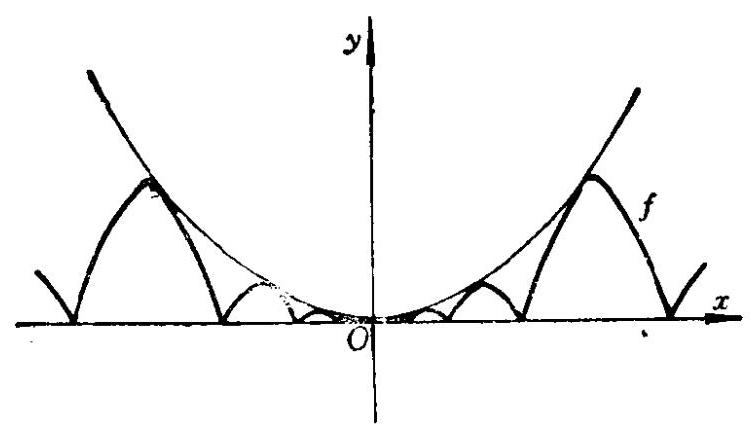
\includegraphics[max width=0.6\textwidth]{images/bo_d25ksc77aajc738obdgg_439_426_264_751_430_0.jpg}
\end{center}
\hspace*{3em} 

图 8-1

对 $x = \frac{1}{2k\pi }$ : 由于
\begin{align*}
	&{f}^{\prime }\left( {\frac{1}{2k\pi }}^{ + }\right)  = \mathop{\lim }\limits_{{x \rightarrow  {\frac{1}{2k\pi }}^{ + }}}\frac{f\left( x\right)  - f\left( \frac{1}{2k\pi }\right) }{x - \frac{1}{2k\pi }}\\
	&= \mathop{\lim }\limits_{{x \rightarrow  \frac{1}{2k\pi }}}\frac{-{x}^{2}\sin \frac{1}{x}}{x - \frac{1}{2k\pi }}\\
	&= \mathop{\lim }\limits_{{x \rightarrow  \frac{1}{2k\pi }}}\left( {-{2x}\sin \frac{1}{x} + \cos \frac{1}{x}}\right)\\
	&= 1\text{ , }\\
	&{f}^{\prime }\left( {\frac{1}{2k\pi }}^{ - }\right)  = \mathop{\lim }\limits_{{x \rightarrow  \frac{1}{2k\pi }}}\frac{f\left( x\right)  - f\left( \frac{1}{2k\pi }\right) }{x - \frac{1}{2k\pi }}\\
	&= \mathop{\lim }\limits_{{x \rightarrow  \frac{1}{2k\pi }}}\frac{{x}^{2}\sin \frac{1}{x}}{x - \frac{1}{2k\pi }}\\
	&= \mathop{\lim }\limits_{{x \rightarrow  \frac{1}{2k\pi }}}\left( {{2x}\sin \frac{1}{x} - \cos \frac{1}{x}}\right)\\
	&=  - 1\text{ , }
\end{align*}

故 $x = \frac{1}{2k\pi }$ 是 $f$ 的不可导点.

对 $x = \frac{1}{\left( {{2k} + 1}\right) \pi }$ ,同理可证 $x = \frac{1}{\left( {{2k} + 1}\right) \pi }$ 也是 $f$ 的不可导点.

由于 ${f}^{\prime }\left( 0\right)  = 0$ ,故 $f$ 的全部不可导点为 $\frac{1}{k\pi }\left( {k \in  \mathrm{Z}-\{ 0\} }\right)$ . 因为 $f\left( x\right)  \geq  0$ ,故这些不可导点都是 $f$ 的严格局部极小值点.

3) ${f}^{\prime }\left( x\right)  = 0$ 的点:

因为 ${f}^{\prime }\left( 0\right)  = 0$ . 并且 $f\left( 0\right)  = 0$ ,故 $x = 0$ 是 $f$ 的局部极小值点.

对 $x \neq  0$ ,由
$$0 = {F}^{\prime }\left( x\right)  = {\left( {x}^{2}\sin \frac{1}{x}\right) }^{\prime } = {2x}\sin \frac{1}{x} - \cos \frac{1}{x}$$

得到 $\operatorname{tg}\frac{1}{x} = \frac{1}{2} \cdot  \frac{1}{x}$ . 此方程在 $\rbrack  - \frac{2}{\pi },\frac{2}{\pi }\lbrack$ 上无解,在每一个区间 $\left. {\rbrack \frac{1}{{k\pi } + \frac{\pi }{2}},\frac{1}{{k\pi } - \frac{\pi }{2}}}\right\rbrack  \left( {k \in  \mathbf{Z},k \neq   - 1}\right)$ 上存在唯一的解 ${x}_{k}$ . 函数 $F$ 在 ${x}_{k}$ 处或取正的严格局部极大值,或在 ${x}_{k}$ 处取负的严格局部极小值.

因此 ${x}_{k}\left( {k \neq   - 1}\right)$ 是 $f$ 的严格局部极大值点.

上面的定理 $8 \cdot  5 \cdot  2$ 是利用函数的一阶导数来研究函数的局部极值点的存在性. 如果函数有更高阶的导数存在, 则我们有下述局部极值点的判断准则,即定理 $8 \cdot  5 \cdot  3$ .

定理 $8 \cdot  5 \cdot  3$ 设 $X \subset  \mathbf{R}$ 是任一非空集合, ${x}_{0} \in  X$ 是一聚点. 函数 $f : X \rightarrow  \mathbf{R}$ 在 ${x}_{0}$ 处 $n$ 次可导,并且满足条件:
$${f}^{\prime }\left( {x}_{0}\right)  = {f}^{\prime \prime }\left( {x}_{0}\right)  = \cdots  = {f}^{\left( n - 1\right) }\left( {x}_{0}\right)  = 0,{f}^{\left( n\right) }\left( {x}_{0}\right)  \neq  0.$$

1) $n$ 为偶数: 若 ${f}^{\left( n\right) }\left( {x}_{0}\right)  > 0$ ,则 ${x}_{0}$ 是 $f$ 的严格局部极小值点; 若 ${f}^{\left( n\right) }\left( {x}_{0}\right)  < 0$ ,则 ${x}_{0}$ 是 $f$ 的严格局部极大值点.

2) $n$ 为奇数: ${x}_{0}$ 不是局部极值点 (参见图 8-2).

证明 因为 $f$ 在 ${x}_{0}$ 处 $n$ 次可导,故 $f$ 在 ${x}_{0}$ 的邻域内有 $n$ 阶限定展开式
\begin{align*}
	&f\left( x\right)  = f\left( {x}_{0}\right)  + \frac{{f}^{\prime }\left( {x}_{0}\right) }{1!}\left( {x - {x}_{0}}\right)  + \frac{{f}^{\prime \prime }\left( {x}_{0}\right) }{2!}{\left( x - {x}_{0}\right) }^{2} + \cdots\\
	&+ \frac{{f}^{\left( n\right) }\left( {x}_{0}\right) }{n!}{\left( x - {x}_{0}\right) }^{n} + o\left( {\left( x - {x}_{0}\right) }^{n}\right) \;\left( {x \rightarrow  {x}_{0}}\right) .
\end{align*}

由假设 ${f}^{\prime }\left( {x}_{0}\right)  = {f}^{\prime \prime }\left( {x}_{0}\right)  = \cdots  = {f}^{\left( n - 1\right) }\left( {x}_{0}\right)  = 0,{f}^{\left( n\right) }\left( {x}_{0}\right)  \neq  0$ 得到
$$f\left( x\right)  = f\left( {x}_{0}\right)  + \frac{{f}^{\left( n\right) }\left( {x}_{0}\right) }{n!}{\left( x - {x}_{0}\right) }^{n} + o\left( {\left( x - {x}_{0}\right) }^{n}\right) \;\left( {x \rightarrow  {x}_{0}}\right) ,$$

或 $f\left( x\right)  - f\left( {x}_{0}\right)  = \frac{{f}^{\left( n\right) }\left( {x}_{0}\right) }{n!}{\left( x - {x}_{0}\right) }^{n}\left\lbrack  {1 + o\left( 1\right) }\right\rbrack  \left( {x \rightarrow  {x}_{0}}\right)$ .

由此可知,存在 $\delta  > 0$ ,在 $X \cap  \overset{ \circ  }{B}\left( {{x}_{0},\delta }\right)$ 内, $f\left( x\right)  - f\left( {x}_{0}\right)$ 与 $\frac{{f}^{\left( n\right) }\left( {x}_{0}\right) }{n!}{\left( x - {x}_{0}\right) }^{n}$ 同号.

1) $n$ 为偶数: 若 ${f}^{\left( n\right) }\left( {x}_{0}\right)  > 0$ ,则 $\frac{{f}^{\left( n\right) }\left( {x}_{0}\right) }{n!}{\left( x - {x}_{0}\right) }^{n} > 0$ , $\forall x \in  X \cap  \overset{ \circ  }{B}\left( {{x}_{0},\delta }\right)$ ,从而 $f\left( x\right)  > f\left( {x}_{0}\right) ,\forall x \in  X \cap  \overset{ \circ  }{B}\left( {{x}_{0},\delta }\right)$ . 因此 ${x}_{0}$ 是 $f$ 的严格局部极小值点; 若 ${f}^{\left( n\right) }\left( {x}_{0}\right)  < 0$ ,则
$$\frac{{f}^{\left( n\right) }\left( {x}_{0}\right) }{n!}{\left( x - {x}_{0}\right) }^{n} < 0,\;\forall x \in  X \cap  \overset{ \circ  }{B}\left( {{x}_{0},\delta }\right) ,$$

从而 $f\left( x\right)  < f\left( {x}_{0}\right) ,\forall x \in  X \cap  \overset{ \circ  }{B}\left( {{x}_{0},\delta }\right)$ ,因此 ${x}_{0}$ 是 $f$ 的严格局部极大值点.

2) $n$ 为奇数: 这时当 ${f}^{\left( n\right) }\left( {x}_{0}\right)  > 0$ 时
$$\frac{{f}^{\left( n\right) }\left( {x}_{0}\right) }{n!}{\left( x - {x}_{0}\right) }^{n}\left\{  \begin{array}{ll}  > 0, & \forall x \in  X \cap  {\overset{ \circ  }{B}}_{ + }\left( {{x}_{0},\delta }\right) , \\   < 0, & \forall x \in  X \cap  {\overset{ \circ  }{B}}_{ - }\left( {{x}_{0},\delta }\right) . \end{array}\right.$$

因此 ${x}_{0}$ 不是局部极值点. 当 ${f}^{\left( n\right) }\left( {x}_{0}\right)  < 0$ 时,类似可证, ${x}_{0}$ 也不是 $f$ 的局部极值点.

\begin{center}
	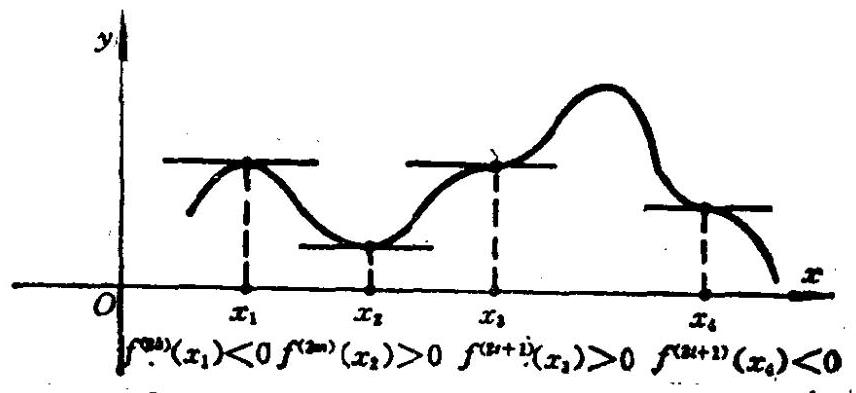
\includegraphics[max width=0.7\textwidth]{images/bo_d25ksc77aajc738obdgg_442_300_367_856_393_0.jpg}
\end{center}
\hspace*{3em} 

图 8-2

例 8 指出正弦函数 $x \mapsto  \sin x,x \in  \mathbf{R}$ 的全部局部极值点及相应的局部极值.

由于 ${\left( \sin x\right) }^{\prime } = \cos x,\forall x \in  \mathbf{R}$ ,故由 $\cos x = 0$ 解得
$${x}_{n} = {n\pi } + \frac{\pi }{2}\;\left( {n \in  \mathbf{Z}}\right) .$$

另一方面,由于 ${\left( \sin x\right) }^{\prime \prime } =  - \sin x$ ,并且
\begin{align*}
	&{\left( \sin x\right) }^{\prime \prime }\left( {x}_{n}\right)  =  - \sin {x}_{n} =  - \sin \left( {{n\pi } + \frac{\pi }{2}}\right)\\
	&= {\left( -1\right) }^{n + 1}\left\{  {\begin{array}{ll}  > 0, & n = {2k} + 1; \\   < 0, & n = {2k}, \end{array}\;k \in  \mathbf{Z}.}\right.
\end{align*}

因此根据定理 $8 \cdot  5 \cdot  3$ 知,正弦函数 $x \mapsto  \sin x,x \in  \mathbf{R}$ 的全部局部极值点为 ${x}_{n} = {n\pi } + \frac{\pi }{2}\left( {n \in  \mathbf{Z},}\right)$ 并且 ${x}_{{2k} + 1} = \left( {{2k} + 1}\right) \pi  + \frac{\pi }{2}\left( {k \in  \mathbf{Z}}\right)$ 是严格局部极小值点,其极小值为 -1,而 ${x}_{2k} = {2k\pi } + \frac{\pi }{2}\left( {k \in  \mathbf{Z}}\right)$ 是严格局部极大值点, 其极大值为 1 .

例9 研究函数
$$x \mapsto  f\left( x\right)  = \left\{  \begin{array}{l} {e}^{-\frac{1}{{x}^{2}}},x \neq  0, \\  0,x = 0 \end{array}\right.$$

的局部极值点.

由于 ${f}^{\prime }\left( x\right)  = \frac{2}{{x}^{3}}{e}^{-\frac{1}{{x}^{2}}},\forall x \neq  0$ ,故 $f$ 在 $\mathbf{R} - \{ 0\}$ 上没有局部极值点.

对 $x = 0$ ,因我们在第 6 章 $§2$ 的例 8 中已证
$${f}^{\left( n\right) }\left( 0\right)  = 0,\;\forall n \in  \mathbf{N}.$$

故对 $x = 0$ ,定理 $8 \cdot  5 \cdot  3$ 不适用. 然而由于
$$f\left( x\right)  > f\left( 0\right)  = 0,\;\forall x \neq  0,$$

故直接由定义知, $x = 0$ 是此函数的严格局部极小值点,其极小值为 0 .

\section*{3. 函数图形的研究}

\section*{1)函数图形的局部形态}

定理 $8 \cdot  5 \cdot  4$ 设 $x \subset  \mathbf{R}$ 是任一非空集合, ${x}_{0} \in  I$ . 函数 $f : X \rightarrow$  $\mathbf{R}$ 在 ${x}_{0}$ 处 $n$ 次可导,并且满足条件:
$${f}^{\prime \prime }\left( {x}_{0}\right)  = {f}^{\prime \prime }\left( {x}_{0}\right)  = \cdots  = {f}^{\left( n - 1\right) }\left( {x}_{0}\right)  = 0,{f}^{\left( n\right) }\left( {x}_{0}\right)  \neq  0.$$

1) $n$ 为偶数: 若 ${f}^{\left( n\right) }\left( {x}_{0}\right)  > 0\left( { < 0}\right)$ ,则 $f$ 的曲 线 在 点 $\left( {x}_{0}\right.$ , $\left. {f\left( {x}_{0}\right) }\right)$ 的附近位于曲线过此点的切线的上 (下) 方.

2) $n$ 为奇数: 则 $f$ 的曲线在点 $\left( {{x}_{0},f\left( {x}_{0}\right) }\right)$ 的附近位于该点切线的两侧,此时称 $f$ 的曲线在点 $\left( {{x}_{0},f\left( {x}_{0}\right) }\right)$ 处与该点的切线横截相交.

证明 因为 $f$ 在 ${x}_{0}$ 处 $n$ 次可导,并且
$${f}^{\prime \prime }\left( {x}_{0}\right)  = {f}^{\prime \prime }\prime \left( {x}_{0}\right)  = \cdots  = {f}^{\left( n - 1\right) }\left( {x}_{0}\right)  = 0,{f}^{\left( n\right) }\left( {x}_{0}\right)  \neq  0,$$

所以 $f$ 在 ${x}_{0}$ 的邻域内的 $n$ 阶限定展开式为
\begin{align*}
	&f\left( x\right)  = f\left( {x}_{0}\right)  + {f}^{\prime }\left( {x}_{0}\right) \left( {x - {x}_{0}}\right)  + \frac{{f}^{\left( n\right) }\left( {x}_{0}\right) }{n!}{\left( x - {x}_{0}\right) }^{n}\\
	&+ o\left( {\left( x - {x}_{0}\right) }^{n}\right) \;\left( {x \rightarrow  {x}_{0}}\right) .
\end{align*}

因此
\begin{align*}
	&f\left( x\right)  - \left\lbrack  {f\left( {x}_{0}\right)  + {f}^{\prime }\left( {x}_{0}\right) \left( {x - {x}_{0}}\right) }\right\rbrack   = \frac{{f}^{\left( n\right) }\left( {x}_{0}\right) }{n!}{\left( x - {x}_{0}\right) }^{n}\\
	&\left\lbrack  {1 + o\left( 1\right) }\right\rbrack  \;\left( {x \rightarrow  {x}_{0}}\right) .
\end{align*}

由此可知,存在 $\delta  > 0$ 使得 $\forall x \in  X \cap  \overset{ \circ  }{B}\left( {{x}_{0},\delta }\right) ,f\left( x\right)$  $- \left\lbrack  {f\left( {x}_{0}\right)  + {f}^{\prime }\left( {x}_{0}\right) \left( {x - {x}_{0}}\right) }\right\rbrack$ 与 $\frac{{f}^{\left( n\right) }\left( {x}_{0}\right) }{n!}{\left( x - {x}_{0}\right) }^{n}$ 同号.

1) $n$ 为偶数: 若 ${f}^{\left( n\right) }\left( {x}_{0}\right)  > 0$ ,则 $f\left( x\right)  - \left\lbrack  {f\left( {x}_{0}\right)  + {f}^{\prime }\left( {x}_{0}\right) }\right.$  $\left. \left( {x - {x}_{0}}\right) \right\rbrack   > 0,\forall x \in  X \cap  B\left( {{x}_{0},\delta }\right)$ . 由于
$$y = f\left( {x}_{0}\right)  + {f}^{\prime }\left( {x}_{0}\right) \left( {x - {x}_{0}}\right)$$

正好是函数 $f$ 的曲线在点 $\left( {{x}_{0},f\left( {x}_{0}\right) }\right)$ 处的切线 $T$ 的方程,故上述不等式表明在点 $\left( {{x}_{0},f\left( {x}_{0}\right) }\right)$ 的附近, $f$ 的曲线位于切线 $T$ 的上方.

若 ${f}^{\left( n\right) }\left( {x}_{0}\right)  < 0$ ,则 $f\left( x\right)  - \left\lbrack  {f\left( {x}_{0}\right)  + {f}^{\prime }\left( {x}_{0}\right) \left( {x - {x}_{0}}\right) }\right\rbrack   < 0$ ,

$\forall x \in  X \cap  \overset{ \circ  }{B}\left( {{x}_{0},\delta }\right) .$

因此在点 $\left( {{x}_{0},f\left( {x}_{0}\right) }\right)$ 的附近, $f$ 的曲线位于切线 $T$ 的下方.

2) $n$ 为奇数: 这时若 ${f}^{\left( n\right) }\left( {x}_{0}\right)  > 0\left( { < 0}\right)$ ,则
\begin{align*}
	&f\left( x\right)  - \left\lbrack  {f\left( {x}_{0}\right)  + {f}^{\prime }\left( {x}_{0}\right) \left( {x - {x}_{0}}\right) }\right\rbrack\\
	&\left\{  \begin{array}{l}  > 0\left( { < 0}\right) ,\forall x \in  X \cap  {\overset{ \circ  }{B}}_{ + }\left( {{x}_{0},\delta }\right) ; \\   < 0\left( { > 0}\right) ,\forall x \in  X \cap  {\overset{ \circ  }{B}}_{ - }\left( {{x}_{0},\delta }\right) . \end{array}\right.
\end{align*}

因此在 ${x}_{0}$ 的右侧, $f$ 的曲线位于切线 $T$ 的上 (下) 方,而在 ${x}_{0}$ 的左侧, $f$ 的曲线位于切线 $T$ 的下 (上) 方. 故 $f$ 的曲线在点 $\left( {{x}_{0},f\left( {x}_{0}\right) }\right)$ 处与切线 $T$ 横截相交.

\begin{center}
	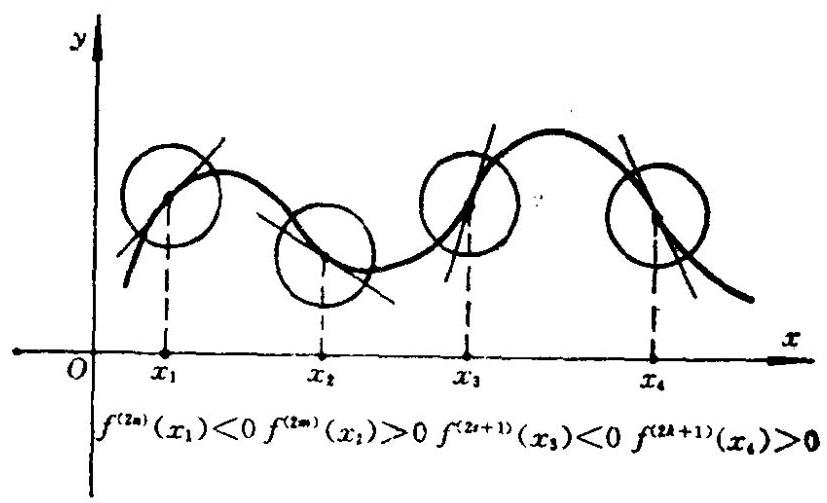
\includegraphics[max width=0.7\textwidth]{images/bo_d25ksc77aajc738obdgg_444_349_1385_827_503_0.jpg}
\end{center}
\hspace*{3em} 

图 8-3

\section*{2 )函数图形的无穷远分支的形态}

在第 5 章 $§4$ 我们定义了函数图形的渐近线. 现在我们利用函数的广义限定展开可以确定函数图形的无穷远分支的渐近线及无穷远分支与渐近线之间的相互位置关系.

例如,设函数 $f : I \rightarrow  \mathbf{R}$ 在 $x =  \pm  \infty$ 邻域内有下述形式的广义限定展开式:
$$f\left( x\right)  = {a}_{0} + {a}_{1}x + \frac{{a}_{2}}{x} + o\left( \frac{1}{x}\right) \left( {x \rightarrow   \pm  \infty }\right) .$$

1) 若 ${a}_{1} = 0$ ,则由 $f\left( x\right)  - {a}_{0} \rightarrow  0\left( {x \rightarrow   \pm  \infty }\right)$ ,知无穷远分支 ${\Gamma }_{+\infty }$ 或 ${\Gamma }_{-\infty }$ 有水平渐近线 $y = {a}_{0}$ .

2) 若 ${a}_{1} \neq  0$ ,则由 $f\left( x\right)  - \left\lbrack  {{a}_{0} + {a}_{1}x}\right\rbrack   \rightarrow  0\left( {x \rightarrow   \pm  \infty }\right)$ 知无穷远分支 ${\Gamma }_{+\infty }$ 或 ${\Gamma }_{-\infty }$ 有斜渐近线 $y = {a}_{0} + {a}_{1}x$ .

在 $\pm  \infty$ 邻域内,若 $\frac{{a}_{2}}{x} > 0\left( { < 0}\right)$ ,则无穷远分支在渐近线 $y = {a}_{0}$  $+ {a}_{1}x$ 的上 (下) 方.

例 10 研究函数 $x \mapsto  f\left( x\right)  = \sqrt[4]{{x}^{4} + {x}^{2}} - \sqrt[3]{{x}^{3} + {x}^{2}},x \in  \mathbf{R}$ 的无穷远分支的渐近线.

首先我们考虑 $x \rightarrow   + \infty$ 时的无穷远分支 ${\Gamma }_{+\infty }$

令 $y = \frac{1}{x}$ . 则
\begin{align*}
	&f\left( x\right)  = \sqrt[4]{\frac{1}{{y}^{4}} + \frac{1}{{y}^{2}}} - \sqrt[3]{\frac{1}{{y}^{3}} + \frac{1}{{y}^{2}}}\\
	&= \frac{1}{y}\left( {\sqrt[4]{1 + {y}^{2}} - \sqrt[3]{1 + y}}\right)\\
	&= \frac{1}{y}\left\lbrack  {1 + \frac{1}{4}{y}^{2} + o\left( {y}^{2}\right)  - 1 - \frac{1}{3}y + \frac{1}{9}{y}^{2} + o\left( {y}^{2}\right) }\right\rbrack\\
	&= \frac{1}{y}\left\lbrack  {-\frac{1}{3}y + \frac{13}{36}{y}^{2} + o\left( {y}^{2}\right) }\right\rbrack\\
	&=  - \frac{1}{3} + \frac{13}{36}y + o\left( y\right)\\
	&=  - \frac{1}{3} + \frac{13}{36}\frac{1}{x} + o\left( \frac{1}{x}\right) \;\left( {x \rightarrow   + \infty }\right) .
\end{align*}

由此可知 $f$ 当 $x \rightarrow   + \infty$ 的无穷远分支 ${\Gamma }_{+\infty }$ 有水平渐近 线 $y =  - \frac{1}{3}$ ,

并且由于在 $+ \infty$ 邻域内 $\frac{13}{36}\frac{1}{x} > 0$ ,故此无穷远分支位于渐近线 $y =  - \frac{1}{3}$ 的上方.

对于 $x \rightarrow   - \infty$ 的无穷远分支 $\Gamma \ldots$ ,由于
\begin{align*}
	&f\left( x\right)  = \sqrt[4]{\frac{1}{{y}^{4}} + \frac{1}{{y}^{2}}} - \sqrt[8]{\frac{1}{{y}^{3}} + \frac{1}{{y}^{2}}}\\
	&=  - \frac{1}{y}\left( {\sqrt[4]{1 + {y}^{2}} + \sqrt[8]{1 + y}}\right)\\
	&=  - \frac{1}{y}\left\lbrack  {1 + \frac{1}{4}{y}^{2} + o\left( {y}^{2}\right)  + 1 + \frac{1}{3}y - \frac{1}{9}{y}^{2} + o\left( {y}^{2}\right) }\right\rbrack\\
	&\left( {y \rightarrow  {0}^{ - }}\right)\\
	&=  - \frac{1}{y}\left\lbrack  {2 + \frac{1}{3}y + \frac{5}{36}{y}^{2} + o\left( {y}^{2}\right) }\right\rbrack\\
	&=  - \frac{1}{3} - {2x} - \frac{5}{36}\frac{1}{x} + o\left( \frac{1}{x}\right) \;\left( {x \rightarrow   - \infty }\right) ,
\end{align*}

故 $f$ 当 $x \rightarrow   - \infty$ 的无穷远分支 ${\Gamma }_{-\infty }$ 有斜渐近线 $y =  - \frac{1}{3} - {2x}$ ,并且由于在 $- \infty$ 邻域内 $- \frac{5}{36}\frac{1}{x} > 0$ ,故此无穷远分支位于渐近线 $y$  $=  - \frac{1}{3} - {2x}$ 的上方.

\section*{3)函数图形的可延展性}

有时出现这种情形: $f$ 在 $a$ 处没有定义,但经过适当的延拓后所得新函数 $\widetilde{f}$ 不仅在点 $a$ 处连续,而且在点 $a$ 处可导.

例11 研究函数 $x \mapsto  f\left( x\right)  = \frac{1}{{e}^{x} - 1} - \frac{1}{x},x \neq  0$ 在 $x = 0$ 处的可延拓性.

利用 ${e}^{x}$ 在 $x = 0$ 的邻域内的限定展开式,我们有
$$\mathop{\lim }\limits_{{x \rightarrow  0}}f\left( x\right)  = \mathop{\lim }\limits_{{x \rightarrow  0}}\frac{1 + x - {e}^{x}}{x\left( {{e}^{x} - 1}\right) } = \mathop{\lim }\limits_{{x \rightarrow  0}}\frac{-\frac{1}{2}{x}^{2} + o\left( {x}^{2}\right) }{x\left( {x + o\left( x\right) }\right) } =  - \frac{1}{2}.$$

若令
$$\widetilde{f}\left( x\right)  = \left\{  \begin{array}{ll} f\left( x\right) , & x \neq  0; \\   - \frac{1}{2}, & x = 0; \end{array}\right.$$

则函数 $\widetilde{f} : \mathbf{R} \rightarrow  \mathbf{R}$ 在 $x = 0$ 处连续,并且在 $x = 0$ 处可导. 事实上,
\begin{align*}
	&\mathop{\lim }\limits_{{x \rightarrow  0}}\frac{\widetilde{f}\left( x\right)  - \widetilde{f}\left( 0\right) }{x} = \mathop{\lim }\limits_{{x \rightarrow  0}}\frac{f\left( x\right)  + \frac{1}{2}}{x}\\
	&= \mathop{\lim }\limits_{{x \rightarrow  0}}\frac{2 + x + \left( {x - 2}\right) {e}^{x}}{2{x}^{2}\left( {{e}^{x} - 1}\right) }\\
	&= \mathop{\lim }\limits_{{x \rightarrow  0}}\frac{2 + x + \left( {x - 2}\right) \left\lbrack  {1 + x + \frac{1}{2}{x}^{2} + \frac{1}{6}{x}^{3} + o\left( {x}^{3}\right) }\right\rbrack  }{2{x}^{2}\left\lbrack  {x + o\left( x\right) }\right\rbrack  }\\
	&= \mathop{\lim }\limits_{{x \rightarrow  0}}\frac{\frac{1}{6}{x}^{3} + o\left( {x}^{3}\right) }{2{x}^{3} + o\left( {x}^{3}\right) }\\
	&= \frac{1}{12},
\end{align*}

因此 $\widetilde{f}$ 在 $x = 0$ 处可导,并且 ${\widetilde{f}}^{\prime }\left( 0\right)  = \frac{1}{12}$ .

最后我们总结上述研究,给出函数作图的步骤.

4)函数作图的具体步骤

1 )确定 $f$ 的定义域 $X$ . 通常 $X$ 是由若干个开区间组成.

2) 计算 ${f}^{\prime }\left( x\right) ,{f}^{\prime \prime }\left( x\right) ,x \in  X$ ,并确定 ${f}^{\prime },{f}^{\prime \prime }$ 的符号变化区间,从而确定 $f$ 的单调性区间及凸凹性区间.

3 )确定 $f$ 的无穷远分支、渐近线及其相互位置.

4 )确定 $f$ 在其定义域 $X$ 的每一个开子区间端点的可延拓性.

5) 列出 $f\left( x\right) ,{f}^{\prime }\left( x\right) ,{f}^{\prime \prime }\left( x\right)$ 的变化表格.

6) 最后画出 $f$ 的简图.

例 12 画出函数 $x \mapsto  f\left( x\right)  = \left( {x - 1}\right) {e}^{\frac{x}{x - 1}}$ 的图形.

1) $f$ 的定义域 $X = 1 - \infty ,1\left\lbrack  \cup \right\rbrack  1, + \infty \lbrack$ .

2) 计算 ${f}^{\prime }\left( x\right)$ 及 ${f}^{\prime \prime }\left( x\right)$ .

直接计算得到
$${f}^{\prime }\left( x\right)  = \frac{x - 2}{x - 1}{e}^{\frac{x}{x - 1}},\;{f}^{\prime \prime }\left( x\right)  = \frac{1}{{\left( x - 1\right) }^{3}}{e}^{\frac{x}{x - 1}}.$$

由此可知:

$\forall x \in  \rbrack  - \infty ,1\left\lbrack  {,{f}^{\prime }\left( x\right)  > 0,{f}^{\prime \prime }\left( x\right)  < 0}\right.$ . 因此 $f$ 在此区间上单调上升, 并且是凹的.

$\forall x \in  \rbrack 1,2\lbrack ,{f}^{\prime }\left( x\right)  < 0,{f}^{\prime \prime }\left( x\right)  > 0$ . 因此 $f$ 在此区间上单调下降, 并且是凸的.

$\forall x \in  \rbrack 2, + \infty \left\lbrack  {,{f}^{\prime }\left( x\right)  > 0,{f}^{\prime \prime }\left( x\right)  > 0}\right.$ . 因此 $f$ 在此区间上单调上升,并且是凸的.

当 $x = 2$ 时, ${f}^{\prime }\left( 2\right)  = 0$ .

3 )确定 $f$ 的无穷远分支及渐近线.

因为
\begin{align*}
	&\mathop{\lim }\limits_{{x \rightarrow  {1}^{ - }}}f\left( x\right)  = \mathop{\lim }\limits_{{x \rightarrow  {1}^{ - }}}\left( {x - 1}\right) {e}^{\frac{x}{x - 1}} = \mathop{\lim }\limits_{{x \rightarrow  {1}^{ - }}}e\left( {x - 1}\right) {e}^{\frac{1}{x - 1}} = 0,\\
	&\mathop{\lim }\limits_{{x \rightarrow  {1}^{ + }}}f\left( x\right)  = \mathop{\lim }\limits_{{x \rightarrow  {1}^{ + }}}\left( {x - 1}\right) {e}^{\frac{x}{x - 1}} = \mathop{\lim }\limits_{{x \rightarrow  {1}^{ + }}}e\left( {x - 1}\right) {e}^{\frac{1}{x - 1}} =  + \infty ,\\
	&\mathop{\lim }\limits_{{x \rightarrow   \pm  \infty }}f\left( x\right)  = \mathop{\lim }\limits_{{x \rightarrow   \pm  \infty }}\left( {x - 1}\right) {e}^{\frac{x}{x - 1}} =  \pm  \infty ,
\end{align*}

所以 $f$ 当 $x \rightarrow  {1}^{ + }$ 及当 $x \rightarrow   \pm  \infty$ 时有无穷远分支 ${\Gamma }_{{1}^{ + }},{\Gamma }_{{1}^{\infty }}$

当 $x \rightarrow  {1}^{ + }$ 的 $f$ 的无穷远分支 ${\Gamma }_{{1}^{ + }}$ 有垂直渐近线 $x = 1$ .

为了研究当 $x \rightarrow   \pm  \infty$ 时 $f$ 的无穷远分支的渐近线,我们对 $f$ 在 $\pm  \infty$ 邻域内作广义的限定展开.
\begin{align*}
	&f\left( x\right)  = e\left( {x - 1}\right) {e}^{\frac{1}{x - 1}}\\
	&= e\left( {x - 1}\right) \left\lbrack  {1 + \frac{1}{x - 1} + \frac{1}{2{\left( x - 1\right) }^{2}} + o\left( \frac{1}{{\left( x - 1\right) }^{2}}\right) }\right\rbrack\\
	&\left( {x \rightarrow   \pm  \infty }\right)\\
	&= {ex} + \frac{e}{2\left( {x - 1}\right) } + o\left( \frac{1}{x - 1}\right) \;\left( {x \rightarrow   \pm  \infty }\right) .
\end{align*}

由此可知当 $x \rightarrow   \pm  \infty$ 时 $f$ 的无穷远分支 ${\Gamma }_{\pm \infty }$ 有斜渐近线 $y = {ex}$ ,并且由于在 $+ \infty$ 邻域内 $\frac{e}{2\left( {x - 1}\right) } > 0$ ,故此无穷 远分支 ${\Gamma }_{+\infty }$ 位于渐近线 $y = {ex}$ 的上方,而由于在 $- \infty$ 邻域内 $\frac{e}{2\left( {x - 1}\right) } < 0$ ,故当 $x \rightarrow$  $- \infty$ 时的无穷远分支 ${\Gamma }_{-\infty }$ 位于渐近线 $y = {ex}$ 的下方.

4) 研究 $f$ 在 $x = 1$ 处可延拓性.

因为
$$\mathop{\lim }\limits_{{x \rightarrow  {1}^{ - }}}f\left( x\right)  = 0,\;\mathop{\lim }\limits_{{x \rightarrow  {1}^{ + }}}f\left( x\right)  =  + \infty ,$$

所以 $f$ 在 $\rbrack  - \infty ,1\lbrack$ 上可连续延拓到 $x = 1$ ,令
$$\widetilde{f}\left( x\right)  = \left\{  \begin{array}{ll} f\left( x\right) , & x \in  \rbrack  - \infty ,1\lbrack ; \\  0, & x = 1, \end{array}\right.$$

则
$$\mathop{\lim }\limits_{{x \rightarrow  {1}^{ - }}}\frac{\widetilde{f}\left( x\right)  - \widetilde{f}\left( 1\right) }{x - 1} = \mathop{\lim }\limits_{{x \rightarrow  {1}^{ - }}}\frac{\left( {x - 1}\right) {e}^{\frac{x}{x - 1}}}{x - 1} = \mathop{\lim }\limits_{{x \rightarrow  {1}^{ - }}}{e}^{\frac{x}{x - 1}} = 0.$$

因此 $\widetilde{f}$ 在 $x = 1$ 处可导,并且 ${\widetilde{f}}^{\prime }\left( 1\right)  = 0$ ,从而 $\widetilde{f}$ 的图形在 $x = 1$ 处有切线 $y = 0$ .

5) 列出 $f\left( x\right) ,{f}^{\prime }\left( x\right) ,{f}^{\prime \prime }\left( x\right)$ 的变化表格.

\begin{center}
	\adjustbox{max width=\textwidth}{
		\begin{tabular}{|c|c|c|c|c|c|}
			\hline
			$x$ & $\left( {-\infty ,1}\right)$ & 1 & (1,2) & 2 & $\left( {2,\; + \infty }\right)$ \\
			\cline{1-6}
			${f}^{\prime }\left( x\right)$ & + & 0 & - & 0 & + \\
			\cline{1-6}
			$f\left( x\right)$ &  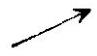
\includegraphics[max width=0.2\textwidth]{images/bo_d25ksc77aajc738obdgg_450_442_518_97_56_0.jpg}  & 0 &  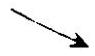
\includegraphics[max width=0.2\textwidth]{images/bo_d25ksc77aajc738obdgg_450_766_518_95_56_0.jpg}  & ${e}^{2}$ &  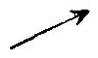
\includegraphics[max width=0.2\textwidth]{images/bo_d25ksc77aajc738obdgg_450_1118_518_98_58_0.jpg}  \\
			\cline{1-6}
			${f}^{\prime \prime }\left( x\right)$ & - & \phantom{X} & + & \phantom{X} & + \\
			\cline{1-6}
			\hline
		\end{tabular}
	}
\end{center}

\begin{center}
	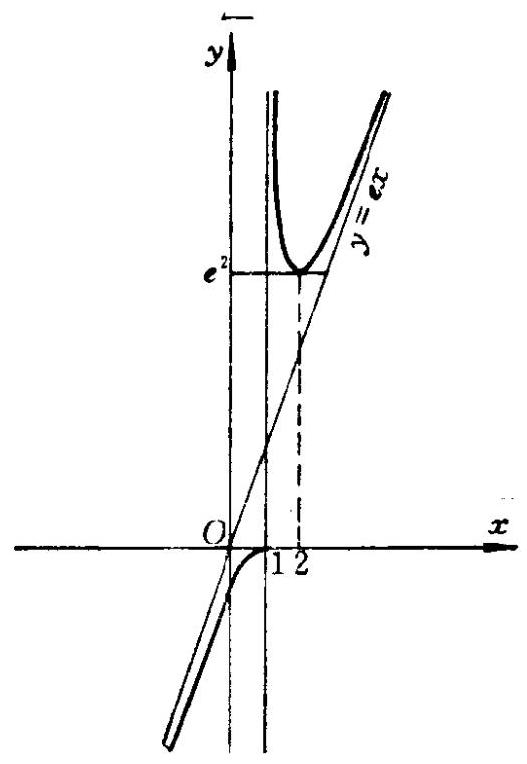
\includegraphics[max width=0.4\textwidth]{images/bo_d25ksc77aajc738obdgg_450_495_774_527_764_0.jpg}
\end{center}
\hspace*{3em} 

图 8-4

\section*{习 题}

1. 计算下列各极限值:

1) $\mathop{\lim }\limits_{{x \rightarrow  0}}\frac{1 - \cos x}{{\operatorname{tg}}^{2}x}$ , 2) $\mathop{\lim }\limits_{{x \rightarrow  0}}\frac{\left( {1 - \cos x}\right) \operatorname{arctg}x}{x{\sin }^{2}x}$ ,

3) $\mathop{\lim }\limits_{{x \rightarrow  0}}\frac{\left( {1 - {e}^{x}}\right) \sin x}{{x}^{2} + {x}^{3}}$ , 4) $\mathop{\lim }\limits_{{x \rightarrow  0}}{\left( \frac{\operatorname{tg}x}{x}\right) }^{\frac{1}{{x}^{2}}}$

5) $\mathop{\lim }\limits_{\substack{\pi \\  x \rightarrow  2 }}{e}^{\frac{1}{\cos x}}\log \frac{2x}{\pi }$ , 6) $\mathop{\lim }\limits_{{x \rightarrow  {0}^{ + }}}{\left( \cos x\right) }^{\frac{1}{{x}^{a}}}\left( {a \geq  0}\right)$ ,

7) $\mathop{\lim }\limits_{{x \rightarrow   + \infty }}\frac{1}{x}\log \frac{{e}^{x} - 1}{x}$ ,

8) $\mathop{\lim }\limits_{{x \rightarrow   + \infty }}x{\left( \log x\right) }^{2}\left\lbrack  {\sin \frac{1}{\log x} - \sin \frac{1}{\log \left( {x + 1}\right) }}\right\rbrack$ ,

9) $\mathop{\lim }\limits_{{x \rightarrow  \infty }}\frac{{x}^{x}\overset{1}{x} - x}{{\left( \log x\right) }^{2}}$ , 10) $\mathop{\lim }\limits_{{x \rightarrow  0}}\frac{1}{{x}^{7}}{\operatorname{tg}}^{3}x\left\lbrack  {{\left( \cos x\right) }^{{x}^{2}} - 1}\right\rbrack$ ,

11) $\mathop{\lim }\limits_{{x \rightarrow  e}}\left( {\log x - 1}\right) \log \left| {x - e}\right|$ ,

12) $\mathop{\lim }\limits_{{x \rightarrow  0}}\frac{{\left( 1 + \sin x\right) }^{\frac{1}{x}} - {e}^{1 - \frac{x}{2}}}{{\left( 1 + \operatorname{tg}x\right) }^{\frac{1}{x}} - {e}^{1 - \frac{x}{2}}}$ ,

13) 确定常数 $a$ 使得 $\mathop{\lim }\limits_{{x \rightarrow  0}}{x}^{a}\left\lbrack  \frac{{\left( \operatorname{sh}\sqrt[3]{x}\right) }^{3} - x}{\sqrt[3]{\operatorname{sh}{x}^{3}} - x}\right\rbrack   = A = 0$ .

2. 求下列各函数 $f$ 的局部极值点与相应的局部极值.

1) $f\left( x\right)  = \sqrt{{2x} - {x}^{2}}$ , 2) $f\left( x\right)  = x + \frac{1}{x}$ ,

3) $f\left( x\right)  = {x}^{x}$ , 4) $f\left( x\right)  = {e}^{\frac{x - 1}{{x}^{2}}}$ ,

5) $f\left( x\right)  = \sqrt[3]{{x}^{3} - {3x} + 2}$ , 6) $f\left( x\right)  = {\left( 1 + \operatorname{tg}x\right) }^{\operatorname{tr}x}$ ,

3. 试求函数
$$x \mapsto  f\left( x\right)  = \left\{  \begin{array}{ll} {x}^{2x}, & x > 0, \\  x + 1, & x \leq  0 \end{array}\right.$$

的局部极值点与局部极值.

4. 设 $n,m \in  \mathbf{N},a > 0$ ,试确定函数
$$x \mapsto  f\left( x\right)  = {x}^{n} \cdot  {\left( a - x\right) }^{m},x \in  \mathbf{R}$$

的局部极值点与局部极值, 并画出图形.

5. 试找出 Riemann 函数
$$x \mapsto  R\left( x\right)  = \left\{  \begin{array}{l} 0,x \in  \rbrack 0,1\lbrack  \cap  {Q}^{i}; \\  \frac{1}{p},x \in  \rbrack 0,1\rbrack  \cap  Q,x = \frac{q}{p},p,q\text{ 互质; } \\  1,x = 0 \end{array}\right.$$

的全部严格局部极大值点.

6. 设 ${a}_{i} \in  R\left( {i = 1,2,\cdots ,n}\right)$ .

1) 求函数 $x \mapsto  f\left( x\right)  = \mathop{\sum }\limits_{{i = 1}}^{n}{\left( x - {a}_{i}\right) }^{2},x \in  \mathrm{R}$ 的局部极小值;

2) 求函数 $x \mapsto  f\left( x\right)  = \mathop{\sum }\limits_{{i = 1}}^{n}{\left| x - {a}_{i}\right| }^{2},x \in  R$ 的局部极小值;

3) 求函数 $x \mapsto  f\left( x\right)  = \mathop{\sum }\limits_{{i = 1}}^{n}{\lambda }_{i}\left| {x - {a}_{i}}\right| ,x \in  R$ 的局部极小值,这里 ${\lambda }_{i} > 0\left( {i = 1,2,\cdots ,n}\right) .$

7. 设函数 $f : \left\lbrack  {a,b}\right\rbrack   \rightarrow  \mathrm{R}$ 在 $\left\lbrack  {a,b}\right\rbrack$ 上连续,并且 $\left\lbrack  {a,b}\right\rbrack$ 的每一点 $x$ 都是 $f$ 的局部极大值点,证明 $f$ 是常值函数.

8. 试 利用反证法及 3 分间套定理证明: 不可能存在一个函数 $f : I \rightarrow  R(I \subset$  $R$ 是一区间),使得 $I$ 的每一点都是 $f$ 的严格局部极大值点.

9. 求函数 $x \mapsto  f\left( x\right)  = {x}^{3} - {3x},x \in  R$ 在集合 $E = \left\{  {x \in  R\left| {\;{x}^{4} + {36} \leq  }\right. }\right.$  $\left. {{13}{x}^{2}}\right\}$ 上的最大值.

10. 画出下列各函数 $f$ 的图形.

1) $f\left( x\right)  = {x}^{2}\operatorname{arctg}\frac{1}{1 + x}$ . 2) $f\left( x\right)  = {e}^{\frac{1}{x}}\sqrt{{x}^{\prime }x + 2}$ ,

3) $f\left( x\right)  = x + \sqrt{{x}^{2} + 1}$ , 4) $f\left( x\right)  = \frac{\log \left| {x - 2}\right| }{\log \left| x\right| }$ .

